\directlua{pdf.setminorversion(6)}
\documentclass[12pt,a4paper,notitlepage]{report} %,openright,twoside scrbook
% \includeonly{paper1}
\usepackage{thesisstyle}
\addbibresource{bib/PhD.bib}
\hyphenation{ESRGAN+}
\uchyph=0 % prevent uppercase hyphenation

\begin{document}

\pagenumbering{Alph}
\begin{titlepage}
    \centering

    \vspace*{48 pt}
    {\large\textbf{Potential Field Geophysics Enhancement Using Contemporary Deep Learning}}

    \vspace{48 pt}
    {\itshape{{\Large Luke Thomas Smith}, BSc, MRes}}

    \vspace{48 pt}
    This thesis is presented for the degree of

    \vspace{14 pt}
    \textbf{Doctor of Philosophy}

    of

    \textbf{The University of Western Australia}

    \vspace{14 pt}
    School of Earth Sciences

    \vspace{72 pt}
    
\includegraphics[scale=0.35]{fig/etc/UWA_FORMAL_PORTRAIT_CMYK}

    \vspace*{\fill}
    2023
\end{titlepage}

% \shipout\null

\pagenumbering{roman}
\setcounter{page}{1}

\addsec[Abstract]{\centering Abstract}
Geophysics examines the petrophysical expression of geology within the Earth and is vital for exploring and understanding mineral systems under cover.
The growing global demand for resources drives new data acquisition, with sensors that return more and higher quality data.
The challenges and opportunities of big data are not unique to the geosciences, and the development of methods and computing to address these are ubiquitous in the contemporary age of deep learning.

Potential field surveying from aircraft provides rapid and extensive coverage of target geology.
These surveys are routinely conducted as pre-competitive regional data acquisition to stimulate exploration, or as targeted investigations by the exploration industry.
% Surveys are also routinely collected on the ground or by satellite, with processing methods and interpretation shared between all forms of acquisition.
The collected data may contain millions of discrete samples scattered in three dimensions, and their interpretation often relies on regularisation to a quantised grid, allowing digital processing and human or machine interpretation.
% A constraint on the usefulness of these data is the data resolution, or more precisely, the Nyquist frequency of the grid.
The limit on information available within gridded data results directly from the spatial sampling density of the originating survey, and the density of cells used to represent the grid raster.
% The well known geophysics rule of thumb, \emph{a grids cell size should be specified as one-quarter to one-fifth of the line spacing}, has long informed the achievable detail in these survey products.
However, sampling density suffers various constraints such as cultural obstructions and budget, leading to the need to fly the fewest number of lines that can still meet the resolution required to interpret target geological features.

This thesis reports on three bodies of work across two topics in geophysics: enhancing the high-frequency content of gridded potential field data using \emph{super-resolution}; and, learning a representative function of a potential field extent using \emph{implicit neural representation}.
The first topic enhances the value of geophysical surveys by predicting high-frequency components in sparsely sampled potential field grids.
The second presents a straightforward neural network framework for high quality grid regularisation and processing.
For each body of work in these topics, real-world geophysical case studies are presented in order to demonstrate the effectiveness and challenges of the method with open access data.
Each body of work extends deep learning methods described in computer science literature the same year as the development of the body of work, to keep pace with rapid advances in the field of machine learning.

In the topic of super-resolution, the first method uses convolutional neural networks to enhance the resolution of real magnetic textures in state magnetic grids at four times scale.
This is further explored in the second body of work, where a baseline model is trained with synthetic potential field grid data and fine-tuned with real-world data to address the lack of survey data with sufficient geological representation, and uses a line spacing derived low-resolution transform.
It quantifies the performance of super-resolution upscaling on real-world low-resolution grids with a line spacing from \SI{320}{\m} to \SI{80}{\m}, and investigates the structural accuracy of the result.

The second topic explores a method for learning a representation of a potential field extent from scattered real-world survey data by a contemporary neural network.
The data-driven approach can extract high-resolution grids from the learned representation, as well as calculate analytical spatial gradients.
Grid rasters and horizontal gradients calculated with the method very closely match their numerical counterparts, however, vertical gradients do not.

Individually, the methods developed in this thesis enhance the information extractable from potential field surveys.
However, together they reflect ongoing advances in deep learning and their extension to challenges and opportunities in geophysics.

\newpage{}
\addsec{Acknowledgements}

I wish to thank a great number of people who have contributed to my journey.

First, to my supervisors:
EJ, for bringing together a team of talented and friendly geodata scientists, and caring deeply for them all.
Tom, who set a high bar with his PhD and immediately set about raising his students to the same level.
Daniel, for the meticulous, concise, and actionable reviews and suggestions.
Naveed, whose perspective was invaluable.

My family in NSW, Andie, Dale, and Robert --- I didn't get to visit as much as I had originally planned in 2019, but we made the most of it! Thanks for the support and encouragement, and imparting all the passions of rocks, computers, and tinkering that I have today.

Tasman, for being a good friend and inspirational colleague for most of my academic career --- looking forward to sharing a project again sometime, somewhere in the future!
Lu, for sharing your incredible amount of geophysics knowledge, incredible cooking, and love of tennis with me.
Matilda, for being a wonderful friend and the best housemate --- Thanks for being silly with me.

My first floor colleagues and fellow tech geeks, David, Daniel, Chris, Minh, and Peter --- Your friendship and knowledge has been a wonderful environment to grow in as a geodata scientist.
And all my SES, CET, and friends beyond: Alex, Anne, Ben, France, Jackson, Jules, Kailah, Lauren, Lauri, Liam, Lilly, Maddie, Maria, Malvina, Nicolas, Ravi, Sean, Sumail, Vickie, and Ze --- Thank you for years of lunches, dinners, beaches, rock climbing, yoga, and all the opportunities to talk rocks that I've been missing.

And to all the teachers throughout my life, both professional and incidental: Thank you.

I love you all.

\bigskip
\noindent This research was supported by a Rio Tinto Iron Ore PhD Scholarship.

\noindent This research was supported by an Australian Government Research Training Program (RTP) Scholarship.
\vfill{}

\epigraph{
    \textit{All collected data had come to a final end. Nothing was left to be collected.}

    \smallskip
    \textit{But all collected data had yet to be completely correlated and put together in all possible relationships.}}{Isaac Asimov}


\newpage{}
\tableofcontents{}
\listoffigures{}

\newpage{}
\addsec[Declarations]{Thesis Declaration}
I, Luke Thomas Smith, certify that:
\begin{itemize}
    \item{}This thesis has been substantially accomplished during enrolment in this degree.
    \item{}This thesis is my own work and does not contain any material previously published or written by another person, except where due reference has been made in the text or Authorship Declaration.
    \item{}This thesis does not contain material which has been submitted for the award of any other degree or diploma in my name, in any university or other tertiary institution.
    \item{}In the future, no part of this thesis will be used in a submission in my name, for any other degree or diploma in any university or other tertiary institution without the prior approval of The University of Western Australia and where applicable, any partner institution responsible for the joint-award of this degree.
    \item{}This thesis does not violate or infringe any copyright, trademark, patent, or other rights whatsoever of any person.
\end{itemize}

\vspace*{20 mm}
\noindent\begin{tabular}{ll}
                               &                           \\[8ex]
    \makebox[100 mm]{\dotfill} & \makebox[30 mm]{\dotfill} \\
    Student Signature          & Date                      \\
\end{tabular}

\newpage{}
% Fix incorrect page numbering on the signed form
\includepdf[pages=-,templatesize={595.276pt}{841.89pt},nup=1x1,scale=1,clip,trim=5mm 36.5mm 5mm 20mm,fitpaper=true,pagecommand={\pagestyle{plain}}]{authorship_declaration_signed.pdf}

\pagenumbering{arabic}
\setcounter{page}{1}
\setcounter{section}{0}
\renewcommand{\thesection}{\arabic{section}}

\chapter{Introduction}
\label{ch:intro}
% \newrefsection{}
% \documentclass[manuscript.tex]{subfiles}
% \documentclass[12pt,a4paper]{report} %,openright,twoside
% \usepackage{thesisstyle}
% \addbibresource{bib/PhD.bib}
% % \setcounter{chapter}{1}
% \begin{document}

The subsurface continuation of exposed geology can be extrapolated and interpolated using structures mapped in surveys of the Earth's naturally occuring potential fields.
Potential field surveys offer low-cost investigations over a large spatial extent, and routinely used for geological mapping and interpretation \parencite{nabighian75thAnniversaryHistorical2005}
For this reason, magnetic field surveys are commonly used by geophysicists for geological mapping and interpretation toward understanding the Earth in three dimensions.
Scattered surveys are widely used when interpolated to grid rasters, and interpreted individually or integrated with many other datasets for predicting the subsurface for processes such as numerical modelling and inversion.
In these tasks, the spatial resolution of the grid is a critical factor in their ability to define geological detail \parencite{islesGeologicalInterpretationAeromagnetic2018}.
The role of high-resolution details in these geophysical methods is becoming more important to exploration as resources are increasingly sought from below sedimentary cover.
Resolution enhancement has seen recent success from the use of deep learning \parencite{moserHitchhikerGuideSuperResolution2023}, however it is not understood if these methods could extend to geophysics data, which are highly distinct from natural images.

\section{Research Aims}
The overall aim of this thesis is to adapt and extend the use of deep learning to improve the processing and enhancement and geophysics data. The three aims of this thesis are as follows:

\begin{itemize}
    \item{} Identifying how deep learning resolution enhancement methods previously developed for natural images are applicable to highly distinct magnetic potential fields data;

    \item{} Constructing a model framework to ensure example based models can be trained incorporating diverse types of geological features manifested in magnetic data, and evaluating the effectiveness the framework with a resolution enhancement technique based on survey line spacing;

    \item{} Evaluating a method for representation learning of potential field survey point data, which can predict a grid directly from point located survey data, as well as grids of the directional derivatives calculated of the learnt function using an automatic differentiation framework.
\end{itemize}

The above aims are investigated using case studies with open access aeromagnetic data provided by Geoscience Australia.

\section{Aeromagnetic surveys}
\label{sec:introgeo}
Airborne surveys of the Earth's magnetic or gravitational potential fields are routinely acquired at a range of scales at different stages of exploration, from pre-competitive regional data to stimulate exploration \parencite{howardAirborneGeophysicalCoverage2004}, to targeted investigations by the exploration industry at the prospect scale of up to several square kilometres.
Surveys may also be collected on the ground, or less commonly in exploration, by ship or satellite, with most processing methods and interpretation shared between all forms of acquisition.
Aeromagnetic surveys are among the lowest cost geophysical method \parencite{dentithGeophysicsMineralExploration2014}, however the cost rapidly increases when surveying at higher resolution due to overheads in flight line sampling.
When acquiring data, aircraft fly straight transect lines at a safe elevation above topography, known as the topography drape.
Surveys are flown with a heading in which data will be acquired along line.
For regional and contemporary surveys this is recommended to be North-South, however early practice was to survey perpendicular to the dominant geological strike, under the expectation of sampling the greatest frequency of change in magnetic intensity \parencite{islesGeologicalInterpretationAeromagnetic2018}.
Higher frequencies with these data diminish with increasing source-sensor distance, therefore the lower the height, the more high-frequency components will be captured by the sensor.
Acquisition along flight lines is sampled at a rate of \qty{10}{\hertz} or greater, which corresponds to an interval of \qty{7}{\m} or shorter at nominal flight speeds of \qty{70}{\m\per\s} \parencite{goodwinAirborneMagneticRadiometric2023}.
The spacing between lines is a factor of the scale of investigation and the cost of acquisition, and regional pre-competitive data in Australia targets state-wide coverage at \qty{400}{\m}, which is generally regarded as the upper limit of usefulness to exploration \parencite{howardAirborneGeophysicalCoverage2004}.
These low-resolution surveys, funded by government geoscience agencies, are a key driver in greenfields exploration and are released as open file data.
Higher-resolution surveys over prospective areas fly lines at closer line spacings, of the order \qty{100}{\m}, in order to resolve greater detail.
The importance of these parameters in relation to resolvable detail will be outlined shortly.
The collected data may contain millions of samples scattered in three dimensions, and interpretation or processing often relies on regularisation to a quantised grid.

\subsection{Survey data regularisation}
\label{sec:introgrids}
Survey data can be interpreted as one dimensional transects, but more commonly they are regularised to a two-dimensional grid raster for interpretation in a process termed gridding.
The resulting interpolated array contains uniformly spaced nodes and is referred to as a grid.
Grids are raster data, where each pixel stores a scalar measurement of a specific property.
In geophysics and throughout this thesis, these are referred to as cells, and the property is a measure of the strength of the magnetic field at a specific location.
The field strength measured is the Total Magnetic Intensity (TMI), which is the vector sum of each directional vector of the potential \parencite{blakelyPotentialTheoryGravity1996}.
This scalar value is recorded in nanotesla and may be negative with an unbounded range that can exceed \qty{50,000}{\nano\tesla} in the Earth's environment.
The location recorded at a sample point is the geographic latitude and longitude, and altitude, acquired with high-precision differential GPS, alongside radar altimeter elevation.
These data may be transformed to a flat projected system, where spatial dimensions are expressed in metres, used throughout this thesis.
There are numerous conventional gridding methods, and novel methods are frequently proposed in the literature.
The simplest use surrounding samples for interpolation, such as choosing the closest sample value or applying a transformation function to the neighbouring samples.
Of those most commonly used in potential field geophysics, these are minimum curvature \parencite{briggsMachineContouringUsing1974}, splines \parencite{bhattacharyyaBicubicSplineInterpolation1969,shureHarmonicSplinesGeomagnetic1982,smithGriddingContinuousCurvature1990}, and equivalent sources \parencite{dampneyEquivalentSourceTechnique1969, solerBetterStrategyInterpolating2020}.
Splines are used in bi-directional gridding, which is well-suited for aeromagnetic surveys, where the sample data are first interpolated in the line parallel direction, and the intermediate product is interpolated in the line perpendicular direction \parencite{dentithGeophysicsMineralExploration2014}.
A method known as kriging is used in other areas of geoscience, such as geochemical mapping, and makes use of statistical properties of the known distribution \parencite{hansenInterpretiveGriddingAnisotropic1993,davis1986statistics}.
Some recently proposed gridding methods include the methods of \textcite{naprstekNewMethodInterpolating2019}, \textcite{xuGravityAnomalyReconstruction2019}, or \textcite{chenPotentialFieldData2022}.
Each interpolation method attempts to predict regularly spaced grids by leveraging properties intrinsic to the data, with the possible explicit integration of \emph{a priori} knowledge such as geophysical laws or geological context.
A review of spatial interpolation methods is provided in \textcite{liReviewComparativeStudies2011}.

\subsection{A definition for geophysical resolution}
In interpolated grids the spatial dimension of each cell is referred to as the cell size, with a unit of metre used in this thesis.
As previously stated, resolvable detail in geophysical surveys is a product of the distance between the causative magnetic body and sensor (height), and the line spacing \parencite{islesRelationshipsGeologicalResolution1992,islesGeologicalInterpretationAeromagnetic2018,dentithGeophysicsMineralExploration2014}.
Height is easily controlled by flying the lowest safe and sufficiently smooth topography drape, and along-line sampling is performed at a constant high rate, so the key factor controlling resolution in aeromagnetic survey design is the line spacing.
Further survey design considerations for airborne geophysics are outlined in \textcite{goodwinAirborneMagneticRadiometric2023,islesGeologicalInterpretationAeromagnetic2018,reidAeromagneticSurveyDesign1980}.
Each gridding method includes a final cell size parameter selectable by the geophysicist, with a long-standing guideline of one third to one fifth the line spacing.
This sufficiently preserves detail in areas of high sampling, while avoiding excessive interpolated cells in areas of low sampling, which may lead to artefacts.
Because of the sampling frequency of nominally \qty{7}{\m} in the flight line direction, and  up to \qty{400}{\m} in the line perpendicular direction, the resulting grid resolution will be anisotropic at best, and uniformly low-resolution at worst.
An important property of sampled data is the Nyquist frequency, \[f_{Nyquist} = f_{sampling} / 2.\]
This is the lowest frequency at which a bandwidth limited signal may be sufficiently sampled, beyond which higher frequencies will be incorrectly recorded as aliasing.
An aliased signal contains spurious low-frequency features caused by the sampling, not the underlying signal.
This limiting frequency applies to each sampling direction in surveys, as well as the cell size of the grid.
The smallest resolvable feature in each of these can be spatially described by wavelength, as the inverse of frequency.
In low-resolution aeromagnetic surveys of \qty{400}{\m} line spacing, strong variations of magnetic intensity in the line-perpendicular direction  that occur over a distance shorter than \qty{800}{\m} will be aliased.
When gridded at \qty{80}{\m} cell size, the corresponding limit on resolvable detail is features as small as \qty{160}{\m}.
% This choice of cell size will effectively filter out features in the line-parallel direction that vary strongly, from those possibly present at \qty{14}{\m} through to \qty{160}{\m}.
Depending on the complexity of the geological domain, this may cause spatial aliasing in one direction.
This is visible in grids where features take on a blocky or stepped appearance, referred to as a beading artefact, or generally in this thesis as a low-resolution artefact.
Low-resolution gridded aeromagnetic data refers to surveys with a wide line spacing causing a lack of high-frequency details in the line-perpendicular direction, resulting in potential artefacts, and overly smooth or missing details in grid data.

Here, I state the definition of resolution adopted throughout this thesis.

\bigskip{}
\noindent{}\emph{Resolution in potential field geophysics refers to the level of geological detail in potential field grids.}
\bigskip{}

Resolution can be increased by:
\begin{enumerate}
    \item{} High frequencies, caused by geology, being present in the potential field,
    \item{} Capturing these high frequencies during surveying, by sampling at close line spacing and small source-sensor separation,
    \item{} Interpolating sample data with a small enough spatial cell size to preserve these frequencies.
\end{enumerate}

% - How are they used (geo interp, modelling, filtering) (detailed)
% levelling
% geological interpretation
% modelling
%

\section{Traditional methods for enhancing resolution}
As outlined in \Cref{sec:introgrids}, resolution is a product of sample distance and density, and gridded rasters have a specific number of cells in each axis depending on the spatial extent.
Upsampling raster data to larger height and width dimensions is commonplace, and generally performed by numerical image filters such as the cubic spline \parencite{keysCubicConvolutionInterpolation1981} or Lanczos filter \parencite{lanczos1988applied}.
Some of these interpolation methods are the basis of the gridding methods previously outlined, and simply selecting a smaller cell size during gridding is sufficient to achieve a larger image raster.
These filters are adept at imputing the required cell values while preserving the frequency content of the original raster.
However, no attempt is made at accurately increasing the high-frequency components of the raster, which are required by our definition for high-resolution geophysics.
Without sampling at a smaller separation or closer line spacing, it is still possible to increase the high-frequency content of aeromagnetic grids.

The rate at which the power of the component frequencies of the potential field diminish with increasing distance is well known.
Back-calculation can be made to predict the power of these frequencies at a smaller separation, and this is termed downward continuation \textcite{bullardDeterminationMassesNecessary1948,blakelyPotentialTheoryGravity1996}.
The inverse using a larger distance is termed upward continuation, and is useful for reducing potentially unwanted near-surface magnetic detail, or levelling data to a common datum \parencite[e.g.\ open file magnetic data in Australia is available levelled to the AWAGS datum][]{mintyAirborneGeophysicalMapping2011}.
Downward continuation offers the benefit of high-resolution data from low-resolution sampling, and is therefore highly studied \parencite{zuoDownwardContinuationTransformation2020,fediStableDownwardContinuation2002,zhangNumericalSolutionsMeanValue2018,guoPotentialFieldContinuation2020,gangImprovedStableDownward2018,pilkingtonPotentialFieldContinuation2017}.
However, due to the inclusion of sensor noise, the practicable limit of numerical methods is six times the low-resolution cell size.
Recent approaches in machine learning have overcome this limit, alongside alternative methods for enhancing aeromagnetic survey resolution.

\section{Geophysics data in machine learning}
\label{sec:introdata}
% e.g. limited training data to deal with diverse geological features, geology various regionally - different potential fields features and range, etc....
Natural image raster data are ubiquitous in computer vision machine learning.
These are most commonly three channel arrays containing normalised brightness values in the red, green and blue channels.
Resolution in these rasters is typically a product of an imaging system or software defined grid with regular sampling.
Like in geophysics, these raster data have an array height and width, which is referred to as resolution.
However, the lack of spatial quantification for the size of natural images confuses the term with its definition for geophysical resolution.

Resulting from the processes described in \Cref{sec:introgrids}, geophysical rasters are highly distinct from the image data used widely in computer vision.
This includes the number of channels (3 in natural images, 1 in aeromagnetics), range (255 compared to 50,000 or more), and anisotropy of resolution.
Additionally, the features present within these data are highly dissimilar.
While natural images may contain common objects which share high-level features such as eyes, faces, or complex geometry, these data only share low-level features with aeromagnetic data, such as simple line and curve components.
This fact limits the applicability of transfer learning from methods in computer vision machine learning \parencite{tanSurveyDeepTransfer2018} to geoscience data.
These points also raise the uncertainty of methods developed for natural images to be  applicable to geoscience data.

Geoscience data faces a number of challenges distinct from natural images. These have been outlined in \textcite{karpatneMachineLearningGeosciences2019}, and relevant to this work are:
\begin{itemize}
    \item{} Spatio-Temporal Structure: Aeromagnetic grids are spatially corellated, neighbouring cells contain similar values arising from the same causative volume.
    \item{} Multi-Source Multi-Resolution Data: One location may be covered by multiple aeromagnetic surveys with different resolutions, or the same survey may be presented with different levels of processing.
    \item{} Poor Quality of Data: Sample data are subject to numerous sources of noise, which combine to become a significant fraction of the gridded data value, or be present as aliased frequencies.
    \item{} Small Sample Size: While total aeromagnetic coverage in Australia is high, the high-resolution extents are spatially limited and biased by geological domain.
\end{itemize}

Inference on real-world data presents many challenges \parencite{nikolenkoSyntheticDataDeep2021,tremblayTrainingDeepNetworks2018}.
Despite this, case studies are critical in promoting the adoption of applications in geophysics, by demonstrating a methods suitability to the data used within the task of interest.
As such, case studies are investigated for each aim within this thesis.

\subsection{Deep learning context}
\label{sec:introml}
Machine learning (ML) is a very broad family of techniques for learning functions from data.
Artificial neural networks are a subset of techniques in ML, inspired by a model of the biological neuron \parencite{bishopNeuralNetworksPattern1995}.
It has been established that if sufficient conditions are met, neural networks can approximate any function \parencite{hornikMultilayerFeedforwardNetworks1989}.
A mathematical model of a neuron forms the basis of these networks, and the number of neurons within the network and their arrangement are one primary descriptor of a neural network. 
Neurons are paremeterised by a multiplicative weight term, an added bias term, and an activation function to scale the result.
Each neuron applies these operations to the input, which may either be the input data, or the output of earlier neurons.
The objective of training a neural network is to set the values for these for each neuron in the network, such that the trained network (or model) generalises to novel data.
This is performed by back propagation \parencite{rumelhartLearningRepresentationsBackpropagating1988}, a technique to navigate toward the lowest error solution by calculating the rate of improvement resulting from parameter updates.
A practical introduction to the practice of training machine learning is available from \textcite{stevensDeepLearningPyTorch2020}, while a more formal introduction is provided in \textcite{bishopPatternRecognitionMachine2006}.
Many activation functions have been proposed, with the rectified linear unit (ReLU) being used in most tasks throughout this thesis.
The activation function performs scaling but in many classes of activation function it also performs the important task of scaling the result to zero, which can be interpreted as the lack of a specific feature being present \parencite{williamsLogicActivationFunctions1986}.
However, recent work on periodic activation functions such as the sinusoid \parencite{sitzmann2019siren} enable the networks used in Cref{ch:paper3}.
The other primary descriptor of a neural network is its architecture, referring to the configuration of its intermediate layers between the input and output.
These architectures are described below.

If the network architecture provides the capacity to store and retrieve learning, the data and training architecture provide the actual instruction and delivery.
There are broadly two classes of training; supervised and unsupervised learning. 
The super-resolution and representation learning tasks in this thesis are both supervised tasks, where a reference is provided for the network to calculate an objective function of its performance on.
Unsupervised learning does not have a ground truth or target, and instead learns to identify patterns within the data for tasks in clustering, density estimation, and visualisation \parencite{bishopPatternRecognitionMachine2006}.

Deep learning is a field of contemporary machine learning, where multiple layers of feature learning are undertaken between the input to a method and the output.
The current generation of deep learning is reported by review articles to have begun in 2006 \parencite{dengDeepLearningMethods2014,goodfellowDeepLearning2016a}, and has pervaded many industries and research fields.
These review articles contain thorough background on the implementation and practice of various architectures for undertaking deep learing, as well as earlier machine learning or numerical models that can address tasks now approached with deep learning.
The deep learning tasks explored in this thesis are super-resolution (SR) for the objective of upsampling resolution enhancement, and implicit neural representation (INR).
The network architectures implemented in this thesis to address the tasks include convolutional neural networks (CNN), generative adversarial networks (GAN), and multilayer perceptrons (MLP).
A brief introduction to these topics is provided here.

In an image raster, neighbouring pixels define simple features, and these features combine in the wider image to define complex features.
A CNN is formed from stacked layers of small convolutional kernels, commonly in SR with the kernel size of \numproduct{3 x 3} cells.
While training, these low-level kernels learn simple functions, which are convolved with deeper layers to learn increasingly complex patterns across a larger image extent, while widening the receptive field.
CNN methods have long been well suited for raster data in computer vision tasks such as image classification \parencite[e.g.][]{simonyanVeryDeepConvolutional2015} and, more recently, resolution enhancement \parencite[e.g.][]{zhangResidualDenseNetwork2018}.
The earliest application of CNN to SR was demonstrated by \textcite{dongLearningDeepConvolutional2014}, where convolutional layers throughout the depth of a network are used for low-resolution patch extraction, feature mapping, and reconstruction of super-resolved images.
The outputs of each convolutional layer are similar to hand-crafted filters or the feature dictionaries in earlier example-based super-resolution methods \parencite{freemanExamplebasedSuperresolution2002}, but the learnt filters are more numerous and fully learned from the data with the deep learning approach.
Following the success of \parencite{dongLearningDeepConvolutional2014}, many iterative improvements have been made to CNN based SR\@.
These include SRCNN \parencite{dongImageSuperresolutionUsing2016}, RDN \parencite{zhangResidualDenseNetwork2018}, ESRGAN \parencite{wangESRGANEnhancedSuperresolution2018}, and others \parencite{ledigPhotorealisticSingleImage2017,limEnhancedDeepResidual2017}.
% While each of these works contribute unique features to CNN-based super-resolution, they follow a common stacked layer design.
% This comprises a set of initial input feature extraction convolutions, a sequence of convolutional blocks with activations (neurons), some number and arrangement of intermediate residual learning pathways (skip connections), and an upsampling block for feature upscaling and convolving latent features back to image space.
% Once trained, the learnt functions are conditioned to transform low-resolution features into high-resolution features, using the neighbouring input values of the low-resolution grid in the context of filters learnt from the training data.


Recently, CNNs have been surpassed by coordinate multilayer perceptron (CMLP) neural networks in some representation learning tasks, including SR \parencite{chenLearningContinuousImage2021}.
CMLPs specifically use a dataset containing individual input points containing coordinate features, and train to predict individual output feature vectors at those coordinates \parencite[e.g.][]{mildenhallNeRFRepresentingScenes2020}.
Key to the performance of these networks are implicit functions, which parameterise a function learned from training dataset with a neural network analogue.
The network analogue can then be queried for information that fits the learnt function but was not included in the training data.
In this way, CMLP networks learn a signal as a function of its coordinates, and novel signal values can be predicted for coordinates in the continuous domain of the learnt function.

Generative Adversarial Networks \parencite{goodfellowGenerativeAdversarialNets2014} are a learning framework utilising two competing neural networks.
These are termed the generator and the discriminator, and can be any arbitrary networks linked by objective functions.
When best overall performance arises when each network is equally capable in its respective task, i.e.\ when the objective functions of each network are linked by the Nash equilibrium \parencite{salimansImprovedTechniquesTraining2016,lucicAreGANsCreated2018}.
Because the use of a discriminator allows an independent element for predictive capacity, GANs are highly suited for generative modelling, which includes the task of super-resolution.
However, it was considerably challenging to achieve a stable Nash equilibrium \parencite{salimansImprovedTechniquesTraining2016}, causing difficulty in training these networks, and to produce a diverse range of outputs.
Noise injection was later used in this framework as a method to drive diversity \parencite{karrasStylebasedGeneratorArchitecture2018,rakotonirinaESRGANFurtherImproving2020}.

%  introduce learning implicit representation from imagery and their application for imputation, I think it's useful to link this resolution improvement in geophysics as imputation problem.


\section{Machine learning in geoscience}
\label{sec:introgeoml}

Geoscience is a diverse field, with ubiquitous use of raster data.
Machine learning is not new to geoscience, and work has been performed on applications in the field for many years.
Recent reviews have highlighted a rapid increase in machine learning research contributions to Earth science.
The aims of this thesis are related to specific findings in these review articles.
\textcite{bergenMachineLearningDatadriven2019} recommends the development and use of benchmark datasets and identifies opportunities in the use of transfer learning from synthetic data.
This is echoed by \textcite{karpatneMachineLearningGeosciences2019}, who also identify prospective research avenues in theory guided science using physics-guided neural networks, the concept of directly leveraging \emph{a priori} domain knowledge within machine learning models.

Early adoption of SR was seen in satellite and airborne remote sensing, where the data share image features with natural images \parencite{lanarasSuperresolutionSentinel2Images2018,arunConvolutionalNetworkArchitectures2019,kawulokTrainingDeepNetworks2019}, and others.
Hyperspectral data SR are commonly investigated \parencite{yangHyperspectralImageClassification2018,arunCNNBasedSuperResolutionHyperspectral2020}. 
Rock microscopy images have been upsampled with SR \parencite{niuInnovativeApplicationGenerative2020}, and their accuracy compared using domain specific parameter calculation.
SR with physics informed learning has been performed by \textcite{bodeUsingPhysicsinformedEnhanced2021,jiangMeshfreeFlowNetPhysicsConstrainedDeep2020} in the field of fluid dynamics, \textcite{leongDeepBedMapDeepNeural2020} in the field of basement topography, and \textcite{jungbluthSingleframeSuperresolutionSolar2019} in astrophysics.
Additionally, physics informed learning has been performed with multi-physics integration in \textcite{degen3DMultiphysicsUncertainty2022}.
Seismic data has been investigated with SR \parencite{liSuperresolutionSeismicVelocity2021}, and with the removal of noise \parencite{liDeepLearningSimultaneous2021}.

Various potential field gridding \parencite{naprstekApplicationsMachineLearning2019,wangDeepLearningGravity2019a} and downward continuation methods \parencite{liStableDownwardContinuation2023,yeHighprecisionDownwardContinuation2022} have been proposed leveraging neural networks.
Finally, in the recent topic of implicit representation there have been several applications proposed, including geological modelling \textcite{hillierGeoINRImplicitNeural2023}.

Beyond the applications investigated in this thesis, many other machine learning methods have been investigated in geoscience.
These include: clustering of geophysical textures \parencite{grujicGeophysicsNeuralNetworks2019}, prediction of geological map event history \parencite{guo3DGeologicalStructure2021}, automated interpretation of geological data \parencite{waldelandConvolutionalNeuralNetworks2018, babakhinSemisupervisedSegmentationSalt2019,dawsonImpactDatasetSize2023}, seismic data interpolation \parencite{wangDeeplearningbasedSeismicData2018}, and 3D structure, joint inversion, or modelling \parencite{guo3DGeologicalStructure2021,zhihouJointGravityGravity2021},

Additionally, deep learning methods in medical imaging and other scientific disciplines share challenges and modalities with geoscience raster data, including noise, small sample size, multi-source and multi-resolution, and other properties.
Advances in these fields can be explored and adapted in conjunction with work in geoscience.
Feature identification is a common theme in all fields, using deep learning to detect, classify, or segment features of interest to geoscience research. 

These works in geoscience machine learning commonly reiterate the challenge of data acquisition.
One approach to overcoming this and other challenges faced in real-world geoscience data is to use synthetic data.
During this thesis, a large collection of synthetic data became available, containing realistic 3D geological voxel models and 2D geophysical forward models \parencite{jessellNoddyverseMassiveData2022}.
These data present a large amount of uniformly sampled and noise free grids from an unbiased set of geological domains, and may offer a solution to some of these data challenges.

\section{Research Contributions and Thesis Structure}
This thesis is presented as a series of papers which are published or in-preparation for publication.
These are presented in Cref{ch:paper1,ch:paper2,ch:paper3}, each with a brief contextual introduction.
Key findings and contributions of the research are discussed in Cref{ch:discussion}, followed by overall thesis conclusions in Cref{ch:conclusion}.

Cref{ch:paper1} presents published work on an initial investigation into the technique of deep learning super-resolution for magnetic potential field data.
To our knowledge, this chapter presents the first investigation of deep learning super-resolution of gridded magnetic potential field data within the literature.
Two convolutional neural network models namely RDN and ESRGAN from the contemporary literature are implemented \parencite{zhangResidualDenseNetwork2018,limEnhancedDeepResidual2017}.
With uncertainty on the amount of data required to train a SR model for magnetic grids, a dataset comprising readily available high- and low-resolution TMI grid pairs is formed using published state magnetic compilation maps of Western Australia \parencite{brett20MagneticMerged2020}.
These data contain magnetic features and textures from a range of geological domains.
The chapter concludes by observing the success of SR on magnetic features, characterising the performance of the two adapted networks, and recommending the method based on RDN as being more reliable for the SR task.
The primary contribution of Cref{ch:paper1} is establishing the capacity of the SR networks developed for natural images in computer vision to extend to the distinctly different data of low-resolution aeromagnetic geophysics.

Following the findings of the previous chapter, Cref{ch:paper2} addresses the need for more generalisable model training for real-world super-resolution.
It undertakes these aims by training a baseline synthetic model with data from a contemporaneously published collection of magnetic grids forward modelled from realistic geology \parencite{jessellNoddyverseMassiveData2022}, on data from over \num{300} distinct geological histories.
It subsequently fine-tune trains the baseline model on real-world high-resolution state magnetic data.
Furthermore, it adopts advances in the machine learning literature by implementing the LTE network \parencite{leeLocalTextureEstimator2022}.
The proposed method simulates aeromagnetic line sampling of a potential field extent at \qty{320}{\m} and \qty{80}{\m}, which are in the regional and prospect scale respectively.
While the baseline model can generalise to real-world data, some incorrect reconstructions remain.
By fine-tune training the model with transformed real-world state map data, these errors are rectified, and the structural accuracy is improved.

Cref{ch:paper3} reports the use of coordinate multilayer perceptron (CMLP) neural networks for representation learning of a surveyed potential field extent.
With the proposed method, scattered line data can be encoded into the grid, and cells queried at interpolating coordinates to predict regularised grids.
CMLP networks are highly suited for processing spatial data such as point sampled geophysics surveys.
Additionally, spatial derivatives are calculated on the learnt function directly.
%TODO ensure refer back to aims
Both tasks are fundamental to interpretation and processing in geophysics, and by commencing the methods from point sample data, the number of individual processing steps is reduced, and the application is fully trainable.
To our knowledge, this research is the first description of deep learning implicit neural representation for aeromagnetic potential field data in the literature.

Cref{ch:discussion} presents a synthesis discussion for the prior chapters. Given the recency of deep learning super-resolution and implicit neural representation, multiple avenues of future opportunities are identified.
These aim to increase the adoption of super-resolution in geophysics by addressing apprehension toward the reliability of interpretation of the outputs.
A synthesis comparison of the SR networks adapted in Cref{ch:paper1,ch:paper2} is also presented, which prompts questions regarding model and dataset construction.
The use of a priori information well understood to geophysics is also discussed, with potential application in both super-resolution and implicit neural representation.

Finally, overall conclusions are presented in Cref{ch:conclusion}.

\printbibliography{}

% \end{document}

\chapter[Magnetic Grid Resolution Enhancement Using ML]{Magnetic Grid Resolution Enhancement Using Machine Learning}
\label{ch:paper1}
% \newrefsection{}
This chapter has been reproduced from the following peer reviewed publication. Formatting has been adjusted for consistency.

Smith, L., Horrocks, T., Holden, E.-J., Wedge, D., Akhtar, N., 2022. Magnetic grid resolution enhancement using machine learning: A case study from the Eastern Goldfields Superterrane. Ore Geology Reviews 150, 105119.
\url{https://doi.org/10.1016/j.oregeorev.2022.105119}
\documentclass[manuscript.tex]{subfiles}
\begin{document}
% \setcounter{chapter}{1}
\title{Magnetic grid resolution enhancement using machine learning: A case study from the Eastern Goldfields Superterrane}
\author[1*]{Luke Thomas Smith}
\author[1]{Tom Horrocks}
\author[1]{Eun-Jung Holden}
\author[1]{Daniel Wedge}
\author[2]{Naveed Akhtar}
\affil{Centre for Data-Driven Geoscience, School of Earth Sciences, The University of Western Australia (M006), 35 Stirling Highway, 6009 Perth, Australia}
\affil{Department of Computer Science and Software Engineering, The University of Western Australia (M002), 35 Stirling Highway, 6009 Perth, Australia}
\date{2022-09-21}
\maketitle{}

\begin{abstract}
    Densely sampled geophysical surveys are a key driver for mineral exploration, but sample density, and therefore grid resolution, is limited by survey cost.
    Consequently, computational methods are resorted to for upsampling, or `super-resolving', of gridded geophysical survey data.
    However, existing approaches such as interpolation filters do not leverage high-resolution detail from pre-existing geophysical surveys.
    Through the application of state-of-the-art deep learning super-resolution architectures, accurate high-resolution grids are predicted from corresponding low-resolution grid priors.
    Specifically, the \emph{RDN} and \emph{ESRGAN+} neural network architectures, which were originally developed for enhancing images, are applied to enhance magnetic surveys and trained with high-resolution and low-resolution magnetic grids of the same extent.
    \qty{80}{\metre} cell size magnetic grids are upsampled to \qty{20}{\metre} cell size using this method, and predicted value and structural accuracy comparisons to the corresponding ground truth \qty{20}{\metre} grids are presented over two test sites in the Eastern Goldfields Superterrane, Western Australia.
    The method based on \emph{RDN} achieves \qty{53}{\percent} lower error compared to Bicubic interpolation.
    The case study demonstrates that the deep learning approach can improve the resolution and frequency content of geophysical surveys without requiring additional sampling expense, while remaining accurate against known ground truth surveys.
    Super-resolution may assist in the interpretation of low-resolution survey grids, however these upsampled grids cannot perfectly recreate the accuracy of highly sampled surveys gridded at their optimal cell size.
\end{abstract}

\section{Introduction}
\subsection{Resolution in geophysics}
\label{sec:resingeo}
Surveys of the spatial distribution of physical properties of the Earth, such as the magnetic potential field, are common in geoscience.
These point-sampled surveys are typically interpolated onto a grid raster, and when a raster covers a known spatial extent, its resolution can be referred to as spatial resolution, indicating that each pixel covers a quantified area.
Often referred to as high resolution, a fine spatial resolution is critical for representing high frequency components in a gridded raster.
These high frequency components reveal localised variations in the surveyed potential field, which provide additional detail on subsurface geological structures and the potential for mineralisation.
An example of the additional detail provided by a high-resolution grid is provided in \Cref{fig:lrandhr}, which shows an \qty{80}{\metre} cell size Total Magnetic Intensity (TMI) grid (a) compared to a \qty{20}{\metre} TMI grid of the same \qtyproduct{2560 x 2560}{\metre} extent (b), gridded from the same potential field samples, but interpolated to different resolutions.
The increased density of pixels in the high-resolution \qty{20}{\metre} grid allows higher frequencies in the sampled magnetic potential field to be displayed.
These frequencies are irretrievably lost when the high-resolution grid is downsampled to \qty{80}{\metre}.

\begin{figure}[hbt]
    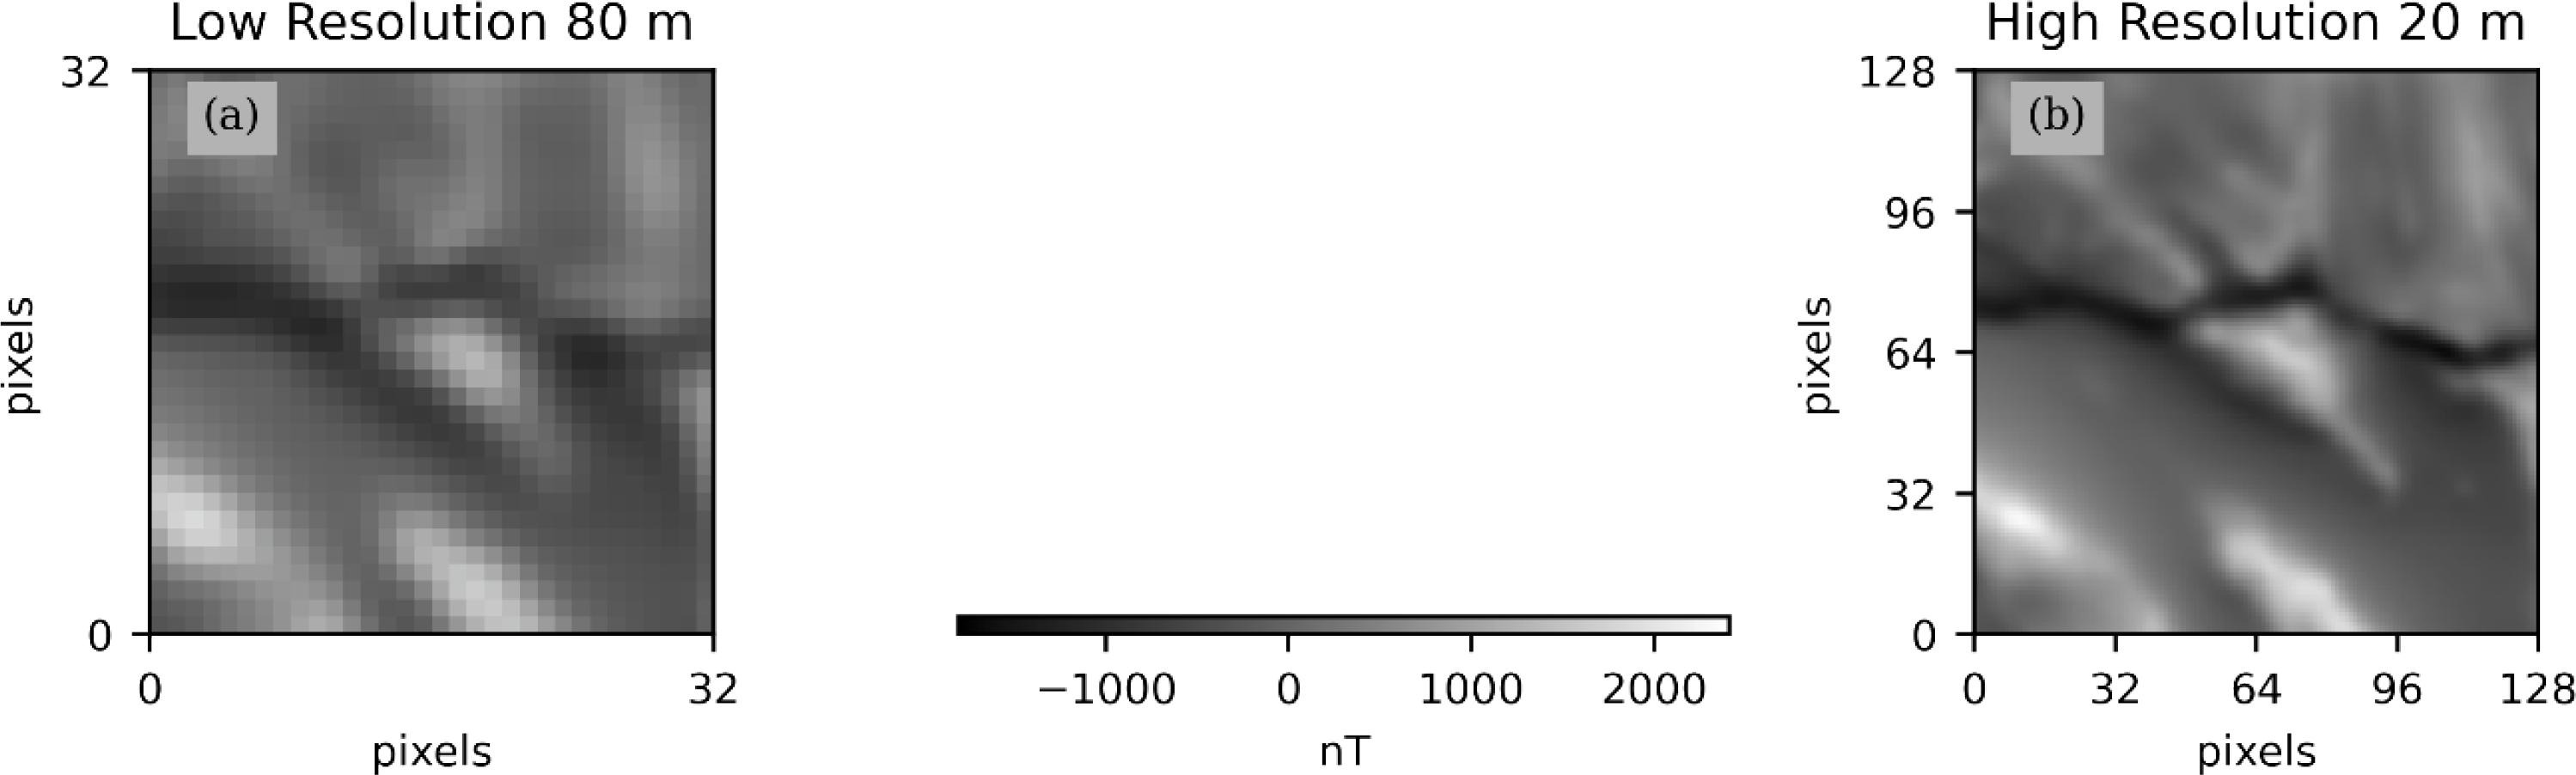
\includegraphics[width=\linewidth]{fig/p1/lrandhr.jpg}
    \caption[Comparison of different resolution grids]{Low resolution \qty{80}{\metre} cell size (a), and high-resolution \qty{20}{\metre} cell size (b) TMI grids over the same extent.
        Each tile is \qtyproduct{2560 x 2560}{\metre}.
        The additional detail shown in the high-resolution grid is made available by the finer cell size, which can convey higher frequency detail, if present in the sampled data.}
    \label{fig:lrandhr}
\end{figure}

Geophysical rasters are created through a process of survey point sampling, grid interpolation, and usually post-process filtering.
During these processes, the sampled potential field may be subject to destructive Nyquist sampling principles \parencite[26]{dentithGeophysicsMineralExploration2014}, especially due to the original point sampling interval and the cell size (pixel spatial extent) selected for the grid interpolation.
The optimal grid cell size is dependent on the sampling interval, and because of this, the highest frequency component preserved in gridded geophysical potential fields is intrinsically limited by the original sampling interval.
This could be summarised as; high frequency components that may be sampled in surveys with close line sampling will be preserved in high-resolution grids with fine cell size.
Typically, cell sizes as fine as one fifth of the line sampling interval can be useful for gridding airborne geophysics \parencite{reidAeromagneticSurveyDesign1980}.
Selecting a cell size finer than one fifth will increase the number of pixels in the image raster, achieving a higher resolution, however no additional geophysical frequencies exist in the point sampled data to be displayed and no detail will be gained.

\subsection{Resolution and frequency}
As discussed in \Cref{sec:resingeo}, a finer spatial resolution grid (fewer metres per pixel) can convey higher frequency information, due to the higher spatial sampling rate.
Indeed, a gridded raster with regularly spaced square cells \(\Delta x\) has an intrinsic Nyquist wavelength \(\lambda _N\), at twice the cell size,

\begin{equation}
    \label{eqn:nyq}
    \lambda{}N = 2 \Delta{}x.
\end{equation}

This corresponds to the shortest wavelength the grid can adequately display, which can be observed as the finest details resolvable in the grid raster.
For example, a high-resolution grid with \qty{20}{\metre} spatial resolution (HR) has a Nyquist wavelength of \qty{40}{\metre}.
In comparison, a low-resolution \qty{80}{\metre} grid (LR) has a Nyquist wavelength of \qty{160}{\metre}.
Note the Nyquist wavelength is proportional between different cell size grids according to the scale factor \(S\),

\begin{equation}
    \label{eqn:hrn}
    \lambda{}N_{HR} = \lambda{}N_{LR} \div{}S.
\end{equation}

Because the highest frequency component preserved in a grid is limited by the grid cell size, any operation that coarsens the cell size is a low pass filter.

\subsection{Improving resolution}
Given the value of higher detail when viewing images, there has been significant research into improving image resolution.
The most straightforward method is to simply sample at a higher rate, which for airborne geophysics means increasing the density of line sampling over a given area.
However, increasing sampling density increases total sampling cost, and cannot easily be done for existing grids.
This paper will investigate a new method for enhancing the resolution of grids by predicting high frequency components in geophysics without requiring additional sampling or cost, based on machine learning methods for image super-resolution.

Recent advances in machine learning techniques for image super-resolution (SR) have been shown to successfully increase image resolution for photographs and other image rasters, while also improving perceptual image quality.
These modern techniques belong to a family of methods known as deep learning, where features learnt early in the network are leveraged to develop a higher understanding of later features.
Notable published examples include SRCNN \parencite{dongLearningDeepConvolutional2014}, VDSR \parencite{kimAccurateImageSuperresolution2016}, SRGAN \parencite{ledigPhotorealisticSingleImage2017}, EDSR \parencite{limEnhancedDeepResidual2017}, RDN \parencite{zhangResidualDenseNetwork2018}, and the current state-of-the-art methods, ESRGAN \parencite{wangESRGANEnhancedSuperresolution2018} and ESRGAN+ \parencite{rakotonirinaESRGANFurtherImproving2020}.
SRGAN and ESRGAN are similar in design to their contemporary counterparts but implement a Generative Adversarial Network (GAN) framework.
In a GAN framework, the upsampling network (termed generator) is trained in an adversarial manner against another network (termed discriminator).
Adversarial training of upsampling networks can help in learning a better model for the task at hand.
For example, ESRGAN uses an analogous upsampling network design to RDN (Residual Dense Network) \Cref{fig:rdn}, with the addition of a discriminator network.
This will be further discussed in \Cref{sec:nnsr}.
For a review on super-resolution networks, the reader is referred to \cite{anwarDeepJourneySuperresolution2020}.

Neural network based super-resolution has seen recent success across many scientific disciplines on data other than natural images.
It is popular in satellite remote sensing \parencite[e.g.][]{lanarasSuperresolutionSentinel2Images2018,wangUltradenseGANSatellite2019}, and has been applied to astrophysics \parencite[e.g.][]{jungbluthSingleframeSuperresolutionSolar2019,salvatelliUsingUNetsCreate2019}, fluid dynamics \parencite{bodeUsingPhysicsinformedEnhanced2021}, elevation models \parencite{leongDeepBedMapDeepNeural2020}, hyperspectral data \parencite[e.g.][]{arunCNNBasedSuperResolutionHyperspectral2020}, and seismic geophysics data \parencite[e.g.][]{liDeepLearningSimultaneous2021,wangDeeplearningbasedSeismicData2018,wangAdaptingResidualDense2022,yuDeepLearningDenoising2019}.
These authors typically report a lower error between the super-resolution upsampled product and ground truth data when compared to a bicubic upsampled product and the ground truth data, as well as improved perceptual quality.
Critically, super-resolution for these applications was able to create realistic high frequency information during upsampling, which could be validated against existing high-resolution surveys of the same extent.
While there are pre-trained models to super-resolve image data (such as ImageNet), the smooth and continuously differentiable nature of potential field data makes it difficult to directly apply such pre-trained models.
For example, it may enhance the appearance of gridding artefacts, instead of supressing them.
While several of the aforementioned works investigate deep learning super-resolution for geospatial data, low resolution in potential field geophysics is a result of under sampling and naïve best-effort interpolation of the potential field, distinct from low-resolution data previously studied in those works.

\begin{figure}[hbt]
    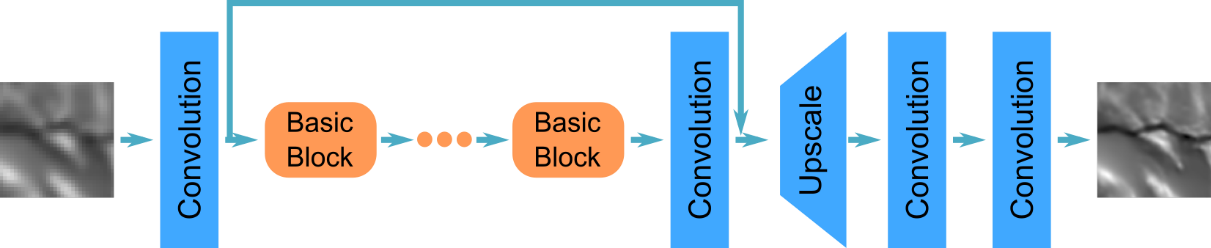
\includegraphics[width=\linewidth]{fig/p1/rdn.png}
    \caption[The RDN architecture]{The RDN architecture, which acts as the ESRGAN generator.
        Twenty-three Basic Blocks are stacked sequentially to form the main convolution path.
        Upsampling to the target output size is performed after the main convolution sequence.
        Adapted from \cite{wangESRGANEnhancedSuperresolution2018}.
    }
    \label{fig:rdn}
\end{figure}

Resolution enhancement in potential field geophysics (occasionally referred to as downward continuation in this context) is performed numerically.
\cite{chenPotentialFieldData2022} use Taylor series expansion, while \cite{xuGravityAnomalyReconstruction2019} interpolate randomly sampled gravity point data using the nonequispaced Discrete Fourier Transform (nDFT), which leverages compressed sensing theory \parencite{candesIntroductionCompressiveSampling2008}.
While high quality results from under sampled data are attained with the non-equispaced Discrete Fourier Transform, the grid line sampling methodology of airborne geophysical surveys is highly regular, and unlikely to satisfy the coherency constraints required for compressive sensing.
This maintains true for data from published grids, which are regularised onto a uniform grid.
To the best of our knowledge, detailed studies on applying and comparing deep learning approaches for geophysical potential field super-resolution has not been previously reported.

\begin{figure}[hbt]
    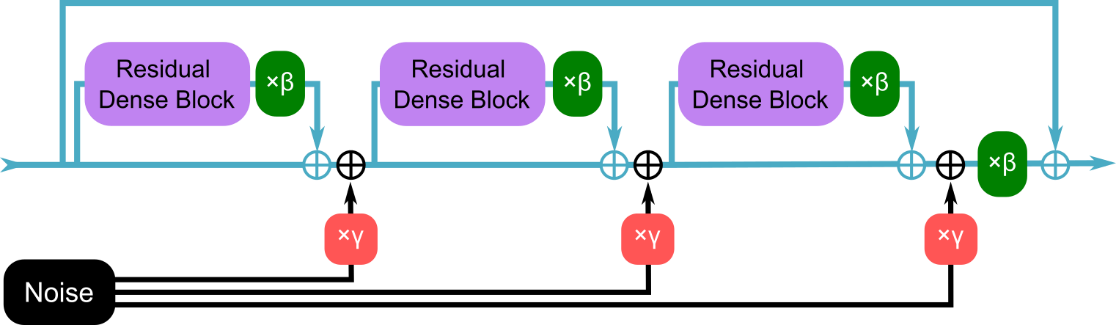
\includegraphics[width=\linewidth]{fig/p1/rdb.png}
    \caption[Basic Blocks]{Each Basic Block (\Cref{fig:rdn}, orange) comprises three weighted Residual Dense Blocks (\Cref{fig:convs}).
        ESRGAN+ extends ESRGAN with the addition of Gaussian Noise after each basic RDB block (black vectors).
        Weight factors are indicated by \(\beta{}\) and \(\gamma{}\).
        Noise injection is not used in RDN\@.
        Adapted from \cite{rakotonirinaESRGANFurtherImproving2020}.
    }
    \label{fig:rdb}
\end{figure}

\begin{figure}[hbt]
    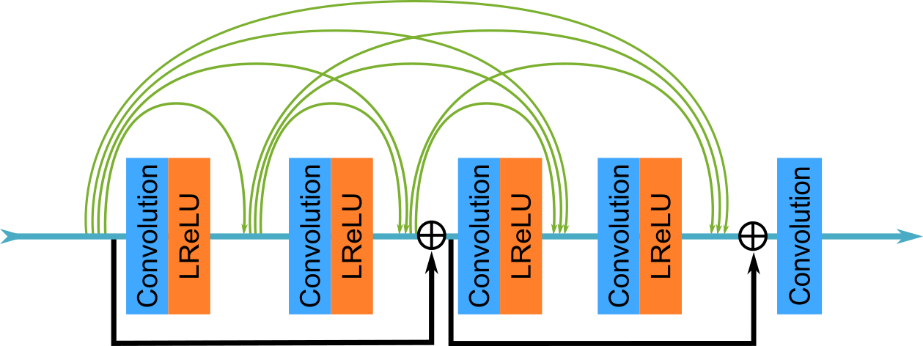
\includegraphics[width=\linewidth]{fig/p1/convs.png}
    \caption[RDB convolutional layers]{Each Residual Dense Block (\Cref{fig:rdb}, purple) comprises four convolutional layers, with additional learning pathways present as residual connections (black), and dense connections (green). LReLU refers to the Leaky-ReLU activation function. Adapted from \cite{rakotonirinaESRGANFurtherImproving2020}.}
    \label{fig:convs}
\end{figure}

\subsection{Interpolation}
Increasing the resolution of an image is achievable through computationally inexpensive interpolating filters, such as nearest neighbour or bicubic interpolation.
These algorithms increase the number of pixels comprising the image raster and predict values for the interpolated pixels.
The nearest neighbour algorithm makes a simple prediction that the value of an interpolated pixel is equal to the nearest ground truth pixel, while the bicubic filter predicts values at interpolated pixels using a cubic function fit to the neighbouring ground truth pixels.
Bicubic interpolation results in a smoothing effect \parencite{keysCubicConvolutionInterpolation1981}, which means it is of limited value for adding higher frequencies to geophysics without additional input data.
It is however suitable as a baseline method to compare upsampling performance against deep learning methods.
It is typical for super-resolution algorithms to use a nearest neighbour upsampling step during their process to achieve the desired output image size, but the upsampled grid is subsequently processed by the neural network to incorporate additional information.
Importantly, basic interpolation is capable of increasing the number of pixels in a grid, but has limited predictive power for high frequency components.
Simply selecting a finer cell size when gridding line sampled data is likely to equal or outperform post-gridding interpolation.

\subsection{Neural network super-resolution}
\label{sec:nnsr}
Convolutional neural network (CNN) upsampling methods use features learned during their training to accurately upscale novel features during inference on novel data.
Learning from an extensive and varied training dataset is a primary driver for the improved performance of CNN methods over simple interpolation methods.
We apply the architectures of two CNN techniques in this work for geophysics super-resolution.
Namely, ESRGAN+ \parencite{rakotonirinaESRGANFurtherImproving2020} which exploits a GAN framework, and a non-GAN variant of the same method which does not rely on the discriminator component of the GAN framework.
The latter has a close resemblance to Residual Dense Network \parencite{zhangResidualDenseNetwork2018} in its architecture.
These CNN models are designed for natural images containing three channel inputs, whereas magnetic and other scientific grids use single channel floating point values.
Hence, for each network it was necessary to change the input array channel count from 3 to 1, and adjust the normalisation method to suit magnetic anomaly values.
We compare these methods to bicubic interpolation to demonstrate the predictive power of the deep learning approaches.

Residual Dense Network (RDN) \parencite{zhangResidualDenseNetwork2018} is a deep learning super-resolution method which consists of a series of residual dense blocks (\Cref{fig:rdb,fig:convs}), which combine the performant residual connections and dense connections (\Cref{fig:convs}) of earlier architectures for state-of-the-art performance.
Residual and dense connections provide additional learning capacity to a CNN, where features learnt in early layers can be fully utilised in later layers.
Following a series of these residual dense blocks, image enlargement is achieved using a simple nearest neighbour interpolation process followed by additional convolution operations.
In this case, enlargement is performed on an intermediate representation of the input, which has gained information during the main network path.
RDN is trained to reduce the Mean Absolute Error L1-norm loss, which corresponds to minimising the absolute difference between the super-resolution prediction and the high-resolution ground truth grid.
RDN was selected as a comparison against ESRGAN+ because RDN is structurally similar to the generator network in ESRGAN, allowing for analysis of the performance of GANs for super-resolution geophysics.
The RDN implementation used here adopts some improvements from ESRGAN+ and will henceforth be referred to as RDN\textdaggerdbl{}.

ESRGAN+, based on ESRGAN \parencite{wangESRGANEnhancedSuperresolution2018}, was chosen as the primary super-resolution CNN architecture for this task due to its reported success in other super-resolution tasks (especially \cite{bodeUsingPhysicsInformedSuperResolution2019} and \cite{leongDeepBedMapDeepNeural2020}) and state of the art results for its original application in image super-resolution.
As a Generative Adversarial Network (GAN), it comprises two iteratively trained neural networks, a Generator (G) used to upscale low-resolution inputs, and Discriminator (D), which is trained to improve the performance of the generator.

G is analogous in design to the RDN architecture described above (\Cref{fig:rdn}), and is trained to upscale a low-resolution input, creating a super-resolution prediction.
The Discriminator network used in ESRGAN is based on a prevalent image classification architecture known as VGG \parencite{simonyanVeryDeepConvolutional2015}.
D is trained to classify its inputs as being either an example of the super-resolved G prediction, or high-resolution ground truth data.
This is used to provide a loss-feedback to G based on G's ability to create realistic SR predictions.
The two networks are trained concurrently, with the contemporaneous D network being used to calculate an adversarial loss for G at each iteration.
The adversarial loss calculated by D is incorporated with the generator's L1 loss as used in RDN, and training continues until D stabilises at 50 \% accuracy where the discriminator is unable to distinguish generated images from real images better than random chance.
At this point, training has converged, and the trained generator model can be used to independently upscale novel inputs.

The specific variant of ESRGAN applied in this work is that of ESRGAN+ \parencite{rakotonirinaESRGANFurtherImproving2020}, which incorporates modern GAN performance improving techniques, including generator noise injection (noted in \Cref{fig:rdb}), and additional dense and residual connections (noted in \Cref{fig:convs}).
These additional connections are used in RDN\textdaggerdbl{}.

The prediction of grid cell values for interpolation is common practice in geophysics.
Existing methods, including nearest neighbour and bicubic filtering, have limited capacity to predict high frequency details to incorporate in upsampled grids, limiting the amount of detail these grids can capture and display.
Recent super-resolution machine learning methods have demonstrated capacity to accurately predict high frequency components in grids from a variety of scientific disciplines, and application of these methods to geophysical potential fields will be investigated here.

\section{Materials and Methods}
\subsection{Geophysical context}
The Eastern Goldfields Superterrane of Western Australia is extensively covered by aeromagnetic surveys of \qty{400}{\metre} line spacing or better, especially over its South-Western extent.
Large survey extents are government sponsored through the Exploration Incentive Scheme \parencite[e.g.][]{griffinStimulatingGreenfieldsExploration2010}, with these low-resolution regional surveys serving to identify prospective areas to undertake surveys at higher resolution.
A number of these higher resolution surveys have been publicly released to open file.
In the Eastern Goldfields the driver for this extensive magnetic coverage is the prominence of highly susceptible BIF and ultramafic formations, which host several major resource projects including Mt Mason (iron ore), Mt Ida and Comet Vale (gold/silver), and Goongarrie (nickel/copper).
A long geological history provides our test region with a variety of magnetic features and textures to test super-resolution performance with, including structurally complex high intensity formations (BIF and ultramafic units), broad textural regions (granites), and extensive linear features (dykes).
Shear zones and fault systems provide further variation to these structures.
Overall, the selected test region in the Eastern Goldfields Superterrane contains sufficient variety of features on which to examine the effect and value of super-resolution upsampling, and determine the suitability of the method for application in other regions.

\subsection{Data}
In typical image SR networks, training data typically take the form of image pairs; the original high-resolution (HR) image, and a low-resolution (LR) image generated on-the-fly by bicubically downsampling the HR image, typically at a scale factor of four.
A similar technique could be used in geophysics SR by applying a low pass filter with a suitable cut-off to a HR grid to simulate the LR counterpart.
However, here we use data from existing grids published at the appropriate four times resolution difference, namely the Magnetic merged grid of Western Australia 2020 at \qty{20}{\metre} (HR) and \qty{80}{\metre} (LR) cell sizes \parencite{brett80MagneticMerged2020}.
When these grids were created, the best available resolution of all grids across the state were compiled at \qty{20}{\metre} cell size, and interpolated to \qty{80}{\metre} using a 4th order Newton polynomial interpolation process \parencite[][personal communication]{brett80MagneticMerged2020}.
This is similar to bicubic interpolation, in that both methods are examples of localised polynomial based interpolation algorithms.
While the cell size is uniform for each respective state grid, the sampling interval of the contributing line surveys varies across the state, which affects the extent of coverage of high frequency components across each grid.
To ensure that the HR ground truth has additional high frequency detail to the LR during training, data were only selected from areas of the Goldfields area of the state grid with contributing survey line spacing \qty{300}{\metre} or closer (optimal cell size strictly finer than \qty{80}{\metre}).
Training and validation data were extracted independent to a reserved test area, outlined in \Cref{fig:trainvaldata}.
By selecting mixed line spacing data in this way, transforms between different scales of frequency loss are captured in the training data.
That is, the same model can learn from fine optimal cell size extents that lose many component frequencies when interpolated to \qty{80}{\metre}, as well as coarse cell size extents which may only lose few or none.
These data were extracted as square tiles, each covering \qty{2560}{\metre} by \qty{2560}{\metre} at 32 \texttimes{} 32 pixels for LR, and 128 \texttimes{} 128 pixels for HR, with no overlap.
This resulted in \num{5290} training tile pairs (used to train the model), \num{512} validation tile pairs (used to select the best performing model), and \num{2415} test tile pairs (used to independently verify the performance of the selected model).
These magnetic grid tiles differ notably from standard colour image tiles, in that they contain 32-bit floating-point values in a single channel, corresponding to the TMI value at each grid cell location.
These values were min-max scaled to a range of 0 to 1 using the global minimum and maximum values of the HR training data.
In summary, the single channel high- and low-resolution state TMI grids were filtered according to a database of their component surveys to extract areas of \qty{300}{\metre} line spacing or less.
These data were normalised according to the statistics of the HR training set, and split into small patches suitable for the hardware limitations.
After application of the architecture under investigation, the data are returned to predicted TMI values, and recompiled into a contiguous spatial extent.

\begin{figure}[hbt]
    \centering{}
    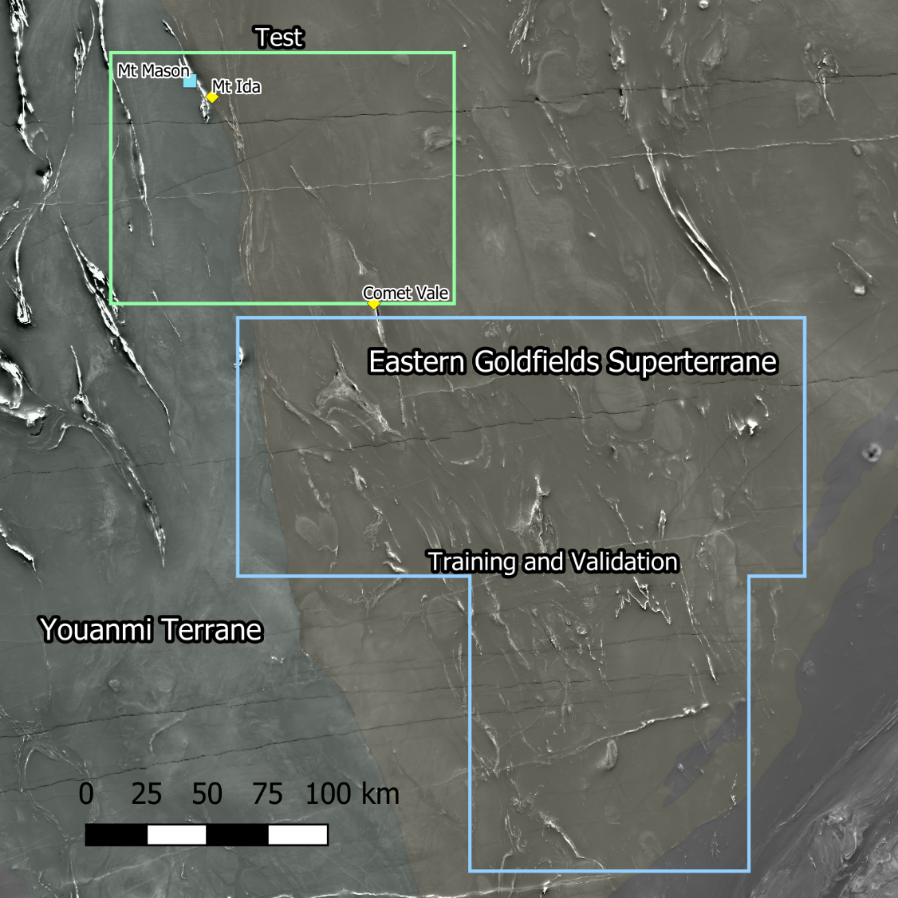
\includegraphics[width=0.75\linewidth]{fig/p1/trainvaldata.png}
    \caption[Dataset context]{Reserved training/validation and test areas of Eastern Goldfields Superterrane magnetic grid, and their tectonic context.
        Background: \qty{20}{\metre} merged magnetic grid of Western Australia, \parencite{brett40MagneticMerged2020}.
    }
    \label{fig:trainvaldata}
\end{figure}

\subsection{Training and inference implementation}
Training of the RDN\textdaggerdbl{} and ESRGAN+ networks was performed with Pytorch \parencite{paszkePyTorchImperativeStyle2019} using an Nvidia RTX 3090 with 24 GB memory, on a desktop computer with an Intel i9-10900KF CPU and 64 GB RAM\@.
Both networks were trained with minibatch size of 64 image patch pairs for \num{602} epochs (\num{17.6} h for RDN\textdaggerdbl{}, \num{21.8} h for ESRGAN+), at which point the PSNR plateaued.
Training samples were augmented using random 90-degree rotations and flips to encourage a model with rotational and symmetrical invariance to the input images, and their order per epoch was shuffled to improve regularisation and supress overfitting.
Further measures for the suppression of overfitting inherent to each of the applied architectures are described in their respective manuscripts \parencite{wangESRGANEnhancedSuperresolution2018,zhangResidualDenseNetwork2018}.
The optimiser used was Adam \parencite{kingmaAdamMethodStochastic2015}.
The learning rate was adjusted over the course of the experiment using the Pytorch implementation of One Cycle Learning Rate scheduler \parencite{smithSuperconvergenceVeryFast2018}, which provides a “warm up” period to stabilise early predictions, and a “cool down” period where the loss minima is fine tuned.
Following the generator implementation from ESRGAN+, twenty-three Residual Dense Blocks were ordered sequentially to form the main network, followed by two nearest neighbour upsampling filters at two times scale each.
The ESRGAN+ discriminator followed that of \cite{rakotonirinaESRGANFurtherImproving2020} which is an implementation of a VGG style classification network \parencite{simonyanVeryDeepConvolutional2015}.
For ESRGAN+ the peak learning rate was \num{6e-4}, and the feature loss, pixel loss (MAE), and adversarial loss parameters were weighted at \num{1}, \num{0.01}, and \num{0.005} respectively.
RDN\textdaggerdbl{} had a peak learning rate of \num{3e-4} and did not require loss component weighting because only L1 pixel loss is used.
Bicubic interpolation was carried out using the implementation provided in Pillow \parencite{vankemenadePythonpillowPillow2021}, a ubiquitous open source Python imaging library.
Inference is carried out using the frozen weights of the trained upsampling models, and takes approximately \num{0.1} s per 32 \texttimes{} 32 pixel tile.
Inference is performed on a tiled basis due to the size of input grids being too large for GPU RAM, and the results may be patched together for full extent visualisation and analysis, or displayed as single tiles.
Predicted outputs are inverse normalised to return the cell values to appropriately scaled TMI units.

\subsection{Accuracy Metrics}
The functional aim of super-resolution geophysics is to accurately predict realistic high frequency details to add to a low-resolution grid.
To quantify this, we calculate root mean square error (RMSE) and structural similarity metrics (SSIM and MS-SSIM), on TMI, high pass filtered TMI, and first vertical derivative (1VD) filtered TMI results for each upsampling method across several sample extents.
Euclidean accuracy measures like RMSE quantify the per-pixel accuracy of a predicted grid compared to its corresponding high-resolution ground truth grid.
For this metric, quality improves as the error value approaches \num{0}.
The Structural Similarity (SSIM) \parencite{wangImageQualityAssessment2004} and Multi-Scale Structural Similarity (MSSSIM) \parencite{wangMultiscaleStructuralSimilarity2003} image quality metrics use sliding windows to quantify image perceptual similarity based on localised structural information.
MS-SSIM extends SSIM by performing a weighted sum of the measure at several different scales.
In both structural metrics, the result is a combination of localised image luminance, contrast, and structural information.
A SSIM value of 1 indicates perfect similarity, and values approaching \num{0} indicate increasing dissimilarity.

\section{Results}
Results are presented to compare the three methods described above, with the metrics of RMSE, SSIM and MS-SSIM, as well as observed perceptual quality.
In addition to unfiltered TMI comparisons, high pass filtered and first vertical derivative TMI grids are also shown.
These products are commonly used in geophysics to investigate high frequency components in grids.

\subsection{Test dataset}
We first present a visual comparison of a selected feature rich \qty{80}{\metre} cell size LR tile, its counterpart \qty{20}{\metre} HR ground truth tile, and the result of; the bicubic upscaling filter, the RDN\textdaggerdbl{} upsampling network, and the ESRGAN+ upsampling network as applied to the LR tile (\Cref{fig:resultsvis}).
This tile was selected from the reserved test region in the Eastern Goldfields Superterrane, and neither of the low- or high-resolution samples were seen during training.
The result of bicubic interpolation (\Cref{fig:resultsvis} c) demonstrates the smoothing effect of the bicubic filter, while the Residual Dense Network (\Cref{fig:resultsvis} d) and ESRGAN+ network (\Cref{fig:resultsvis} e) show added detail.
The two neural network methods more closely match the ground truth \qty{20}{\metre} tile than the bicubic upsampled image does, when observing feature edges and textural detail.


\begin{figure}[hbt]
    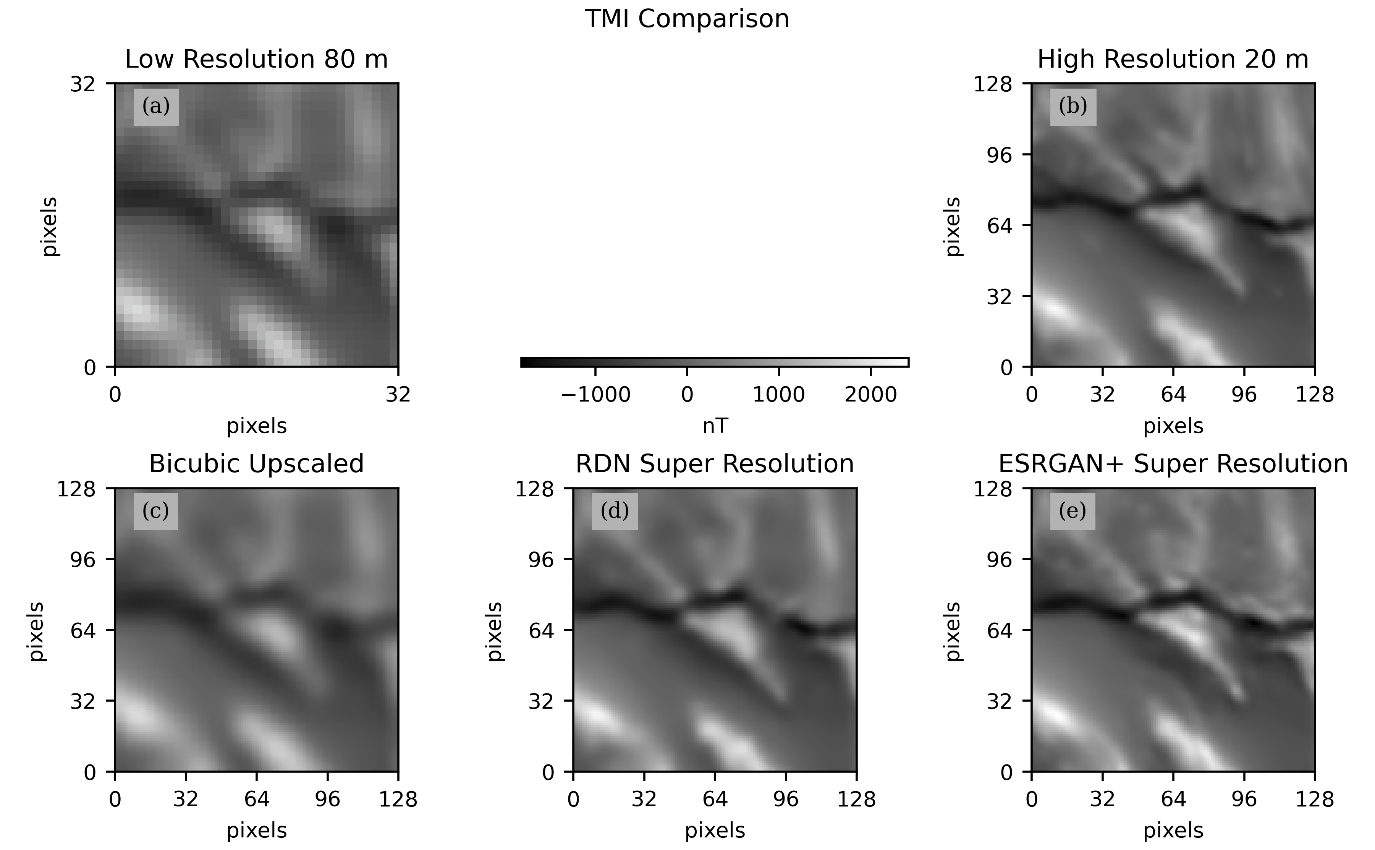
\includegraphics[width=\linewidth,trim={0 0 0 5mm},clip]{fig/p1/resultsvis.png}
    \caption[Visual inference results]{Visual comparisons of a selected tile from the reserved test region.
        The \qty{80}{\metre} low-resolution input (a) is shown at equivalent size to the \qty{20}{\metre} high-resolution ground truth (b) using nearest neighbour interpolation.
        The colourmap is shared between subfigures.
    }
    \label{fig:resultsvis}
\end{figure}

\Cref{fig:residuals} demonstrates the error residuals between the predicted TMI grids for each upsampling method and the HR ground truth.
For the selected tile, the RMSE is best minimised using RDN\textdaggerdbl{}, which also shows the best structural metric performance.
ESRGAN+ outperforms the bicubic method in RMSE and MSSIM\@.

\begin{figure}[hbt]
    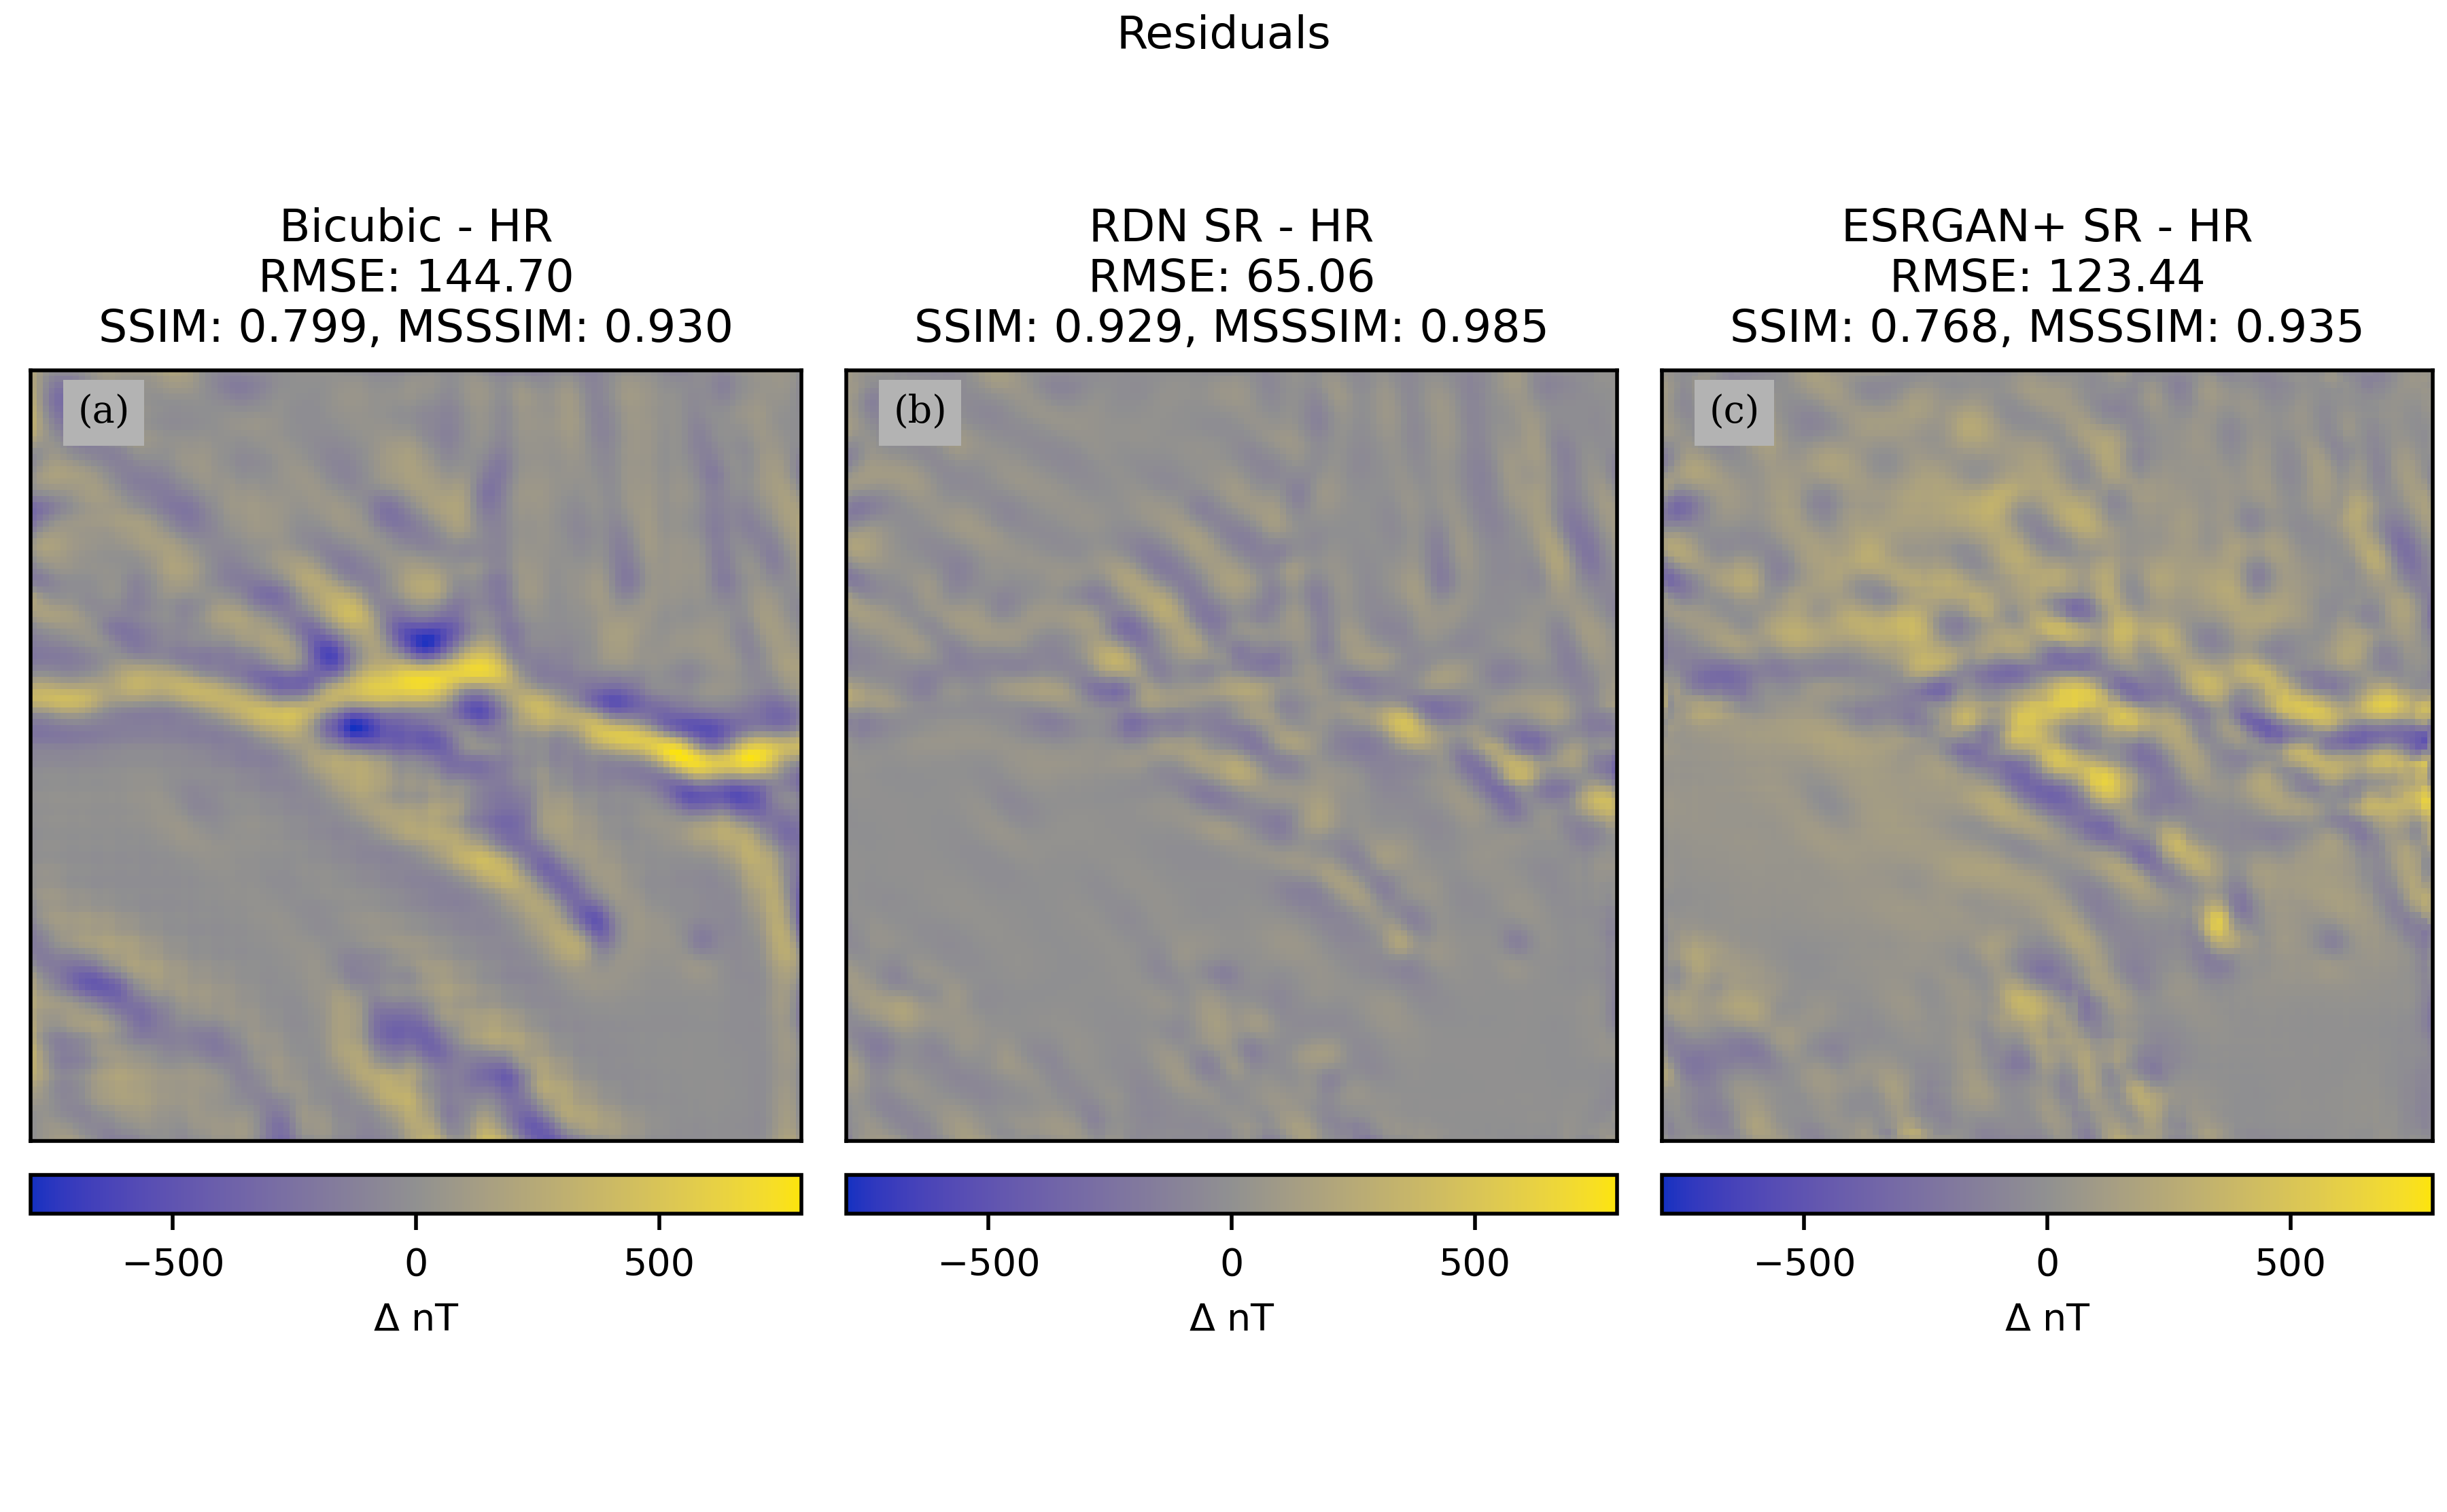
\includegraphics[width=\linewidth,trim={0 10mm 0 5mm},clip]{fig/p1/residuals.png}
    \caption[Error residuals map for a selected tile]{Error residuals map for the selected test tile, for each upsampling method; Bicubic (a), RDN\textdaggerdbl{} (b), and ESRGAN+ (c).
        Image quality metrics are reported for each upsampled tile, calculated against the groundtruth HR\@.}
    \label{fig:residuals}
\end{figure}

The prediction of higher frequencies can be quantified using the Radially Averaged Power Spectral Density.
In the Fourier domain, the amplitudes of an array's component frequencies are mapped to coordinates representing their orientation.
The Radially Averaged Power Spectral Density (RAPSD) \parencite{ulichneyDitheringBlueNoise1988} is a one-dimensional representation of the cumulative power of each frequency component, in any orientation within the image.
\Cref{fig:rapsd} shows the RAPSD for the different methods over the test extent shown in \Cref{fig:trainvaldata}. The deep learning methods have consistently superior power in predicted wavelengths between approximately \qty{640}{\metre} and \qty{120}{\metre}, with RDN\textdaggerdbl{} closely matching the groundtruth spectra, while ESRGAN+ tends to exaggerate.

% TODO USE REVISED MANUSCRIPT FIGURES 

\begin{figure}[hbt]
    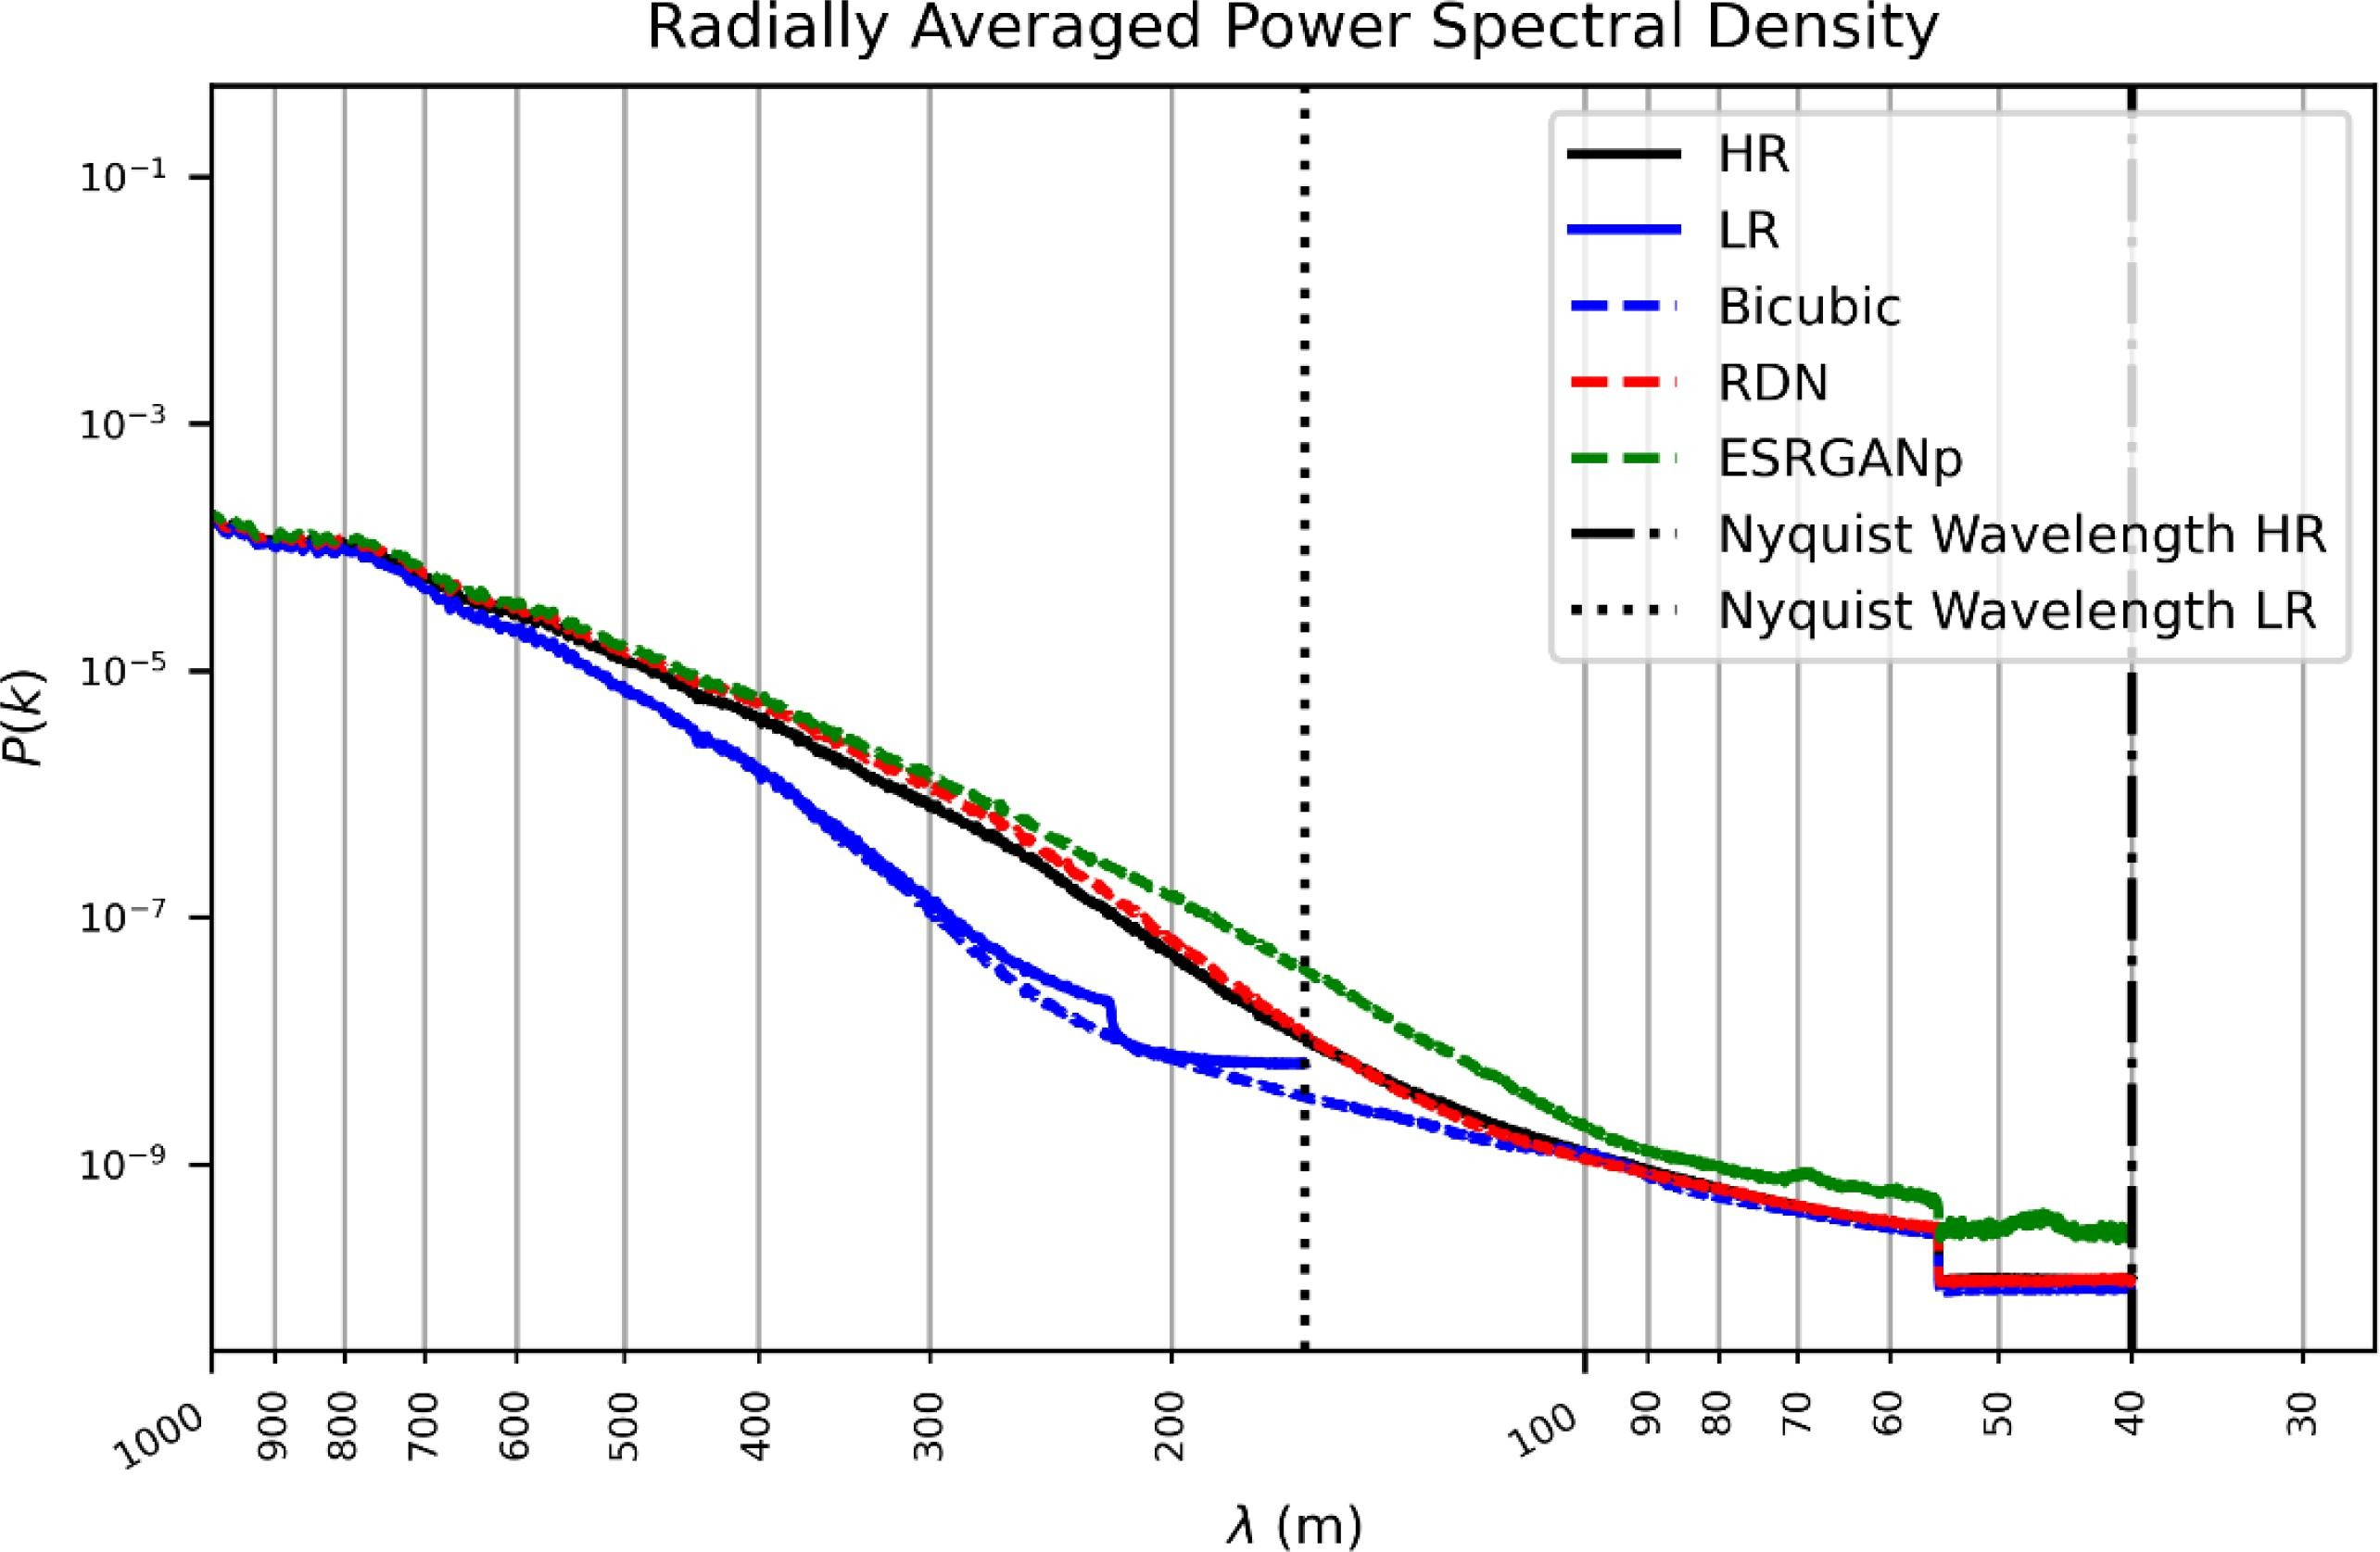
\includegraphics[width=\linewidth]{fig/p1/rapsd.jpg}
    \caption[short]{Radially Averaged Power Spectra for the complete test extent shown in \Cref{fig:trainvaldata}.
        The Nyquist wavelengths for the high-resolution (and upsampled) rasters and low-resolution raster are also shown.
        The frequency axis has been transformed to wavelength, and the spectra have been normalised for direct comparison.
        Note the complete test extent is covered by surveys with a range of line spacings from \qty{100}{\metre} to \qty{20}{\metre}, with \qty{100}{\metre} being the most extensive.
        The Nyquist wavelength of the \qty{100}{\metre} surveys (optimal grid cell size approximately \qty{20}{\metre}) likely causes the reduction in power at \qty{55}{\metre} and \qty{220}{\metre}.
    }
    \label{fig:rapsd}
\end{figure}

To visualise the contribution of these enhanced high frequencies in the resulting grid, the super-resolved output from each method is high pass filtered, with a cut-off wavelength equivalent to the Nyquist wavelength of the LR grid.
By filtering at this wavelength, only frequencies added by the upsampling process will be shown in the output (\Cref{fig:filtered}). Bicubic interpolation (\Cref{fig:filtered} c) fails to add significant high frequency components.
RDN\textdaggerdbl{} (\Cref{fig:filtered} d) appears to approximate similar high frequencies to the HR tile (\Cref{fig:filtered} b), while ESRGAN+ (\Cref{fig:filtered} e) shows potentially excessive predicted high frequency components.
Finally, metrics for the full set of test tiles are reported in \Cref{tab:metrics}.
The non-GAN CNN approach of RDN\textdaggerdbl{} remains the most accurate method for the entire test grid.
Several routinely occurring artefacts are observed in the two super-resolution products, especially in ESRGAN+ which incorporates details it has learned from the Discriminator network loss.
The First Vertical Derivative filter is used in \Cref{fig:jhillvis} to demonstrate the ability to perform common geophysical filters on super resolved grids, and to emphasise examples of these artefacts.
The most apparent artefact arises from the inference implementation when upsampling a grid larger than fits in memory, where visible edges appear around individual tiles in the compiled inference grid (e.g. \Cref{fig:jhillvis}, *).
This could be reduced by adjusting the size of inference tiles, or slightly overlapping adjacent input tiles.
Predictions from ESRGAN+ commonly show a ripple-like texture (\Cref{fig:jhillvis}, \^{ }), especially around pronounced high TMI features.
The effect of this texture occasionally reveals features matching the high-resolution groundtruth that are not predicted by the bicubic or RDN\textdaggerdbl{} upsampling, but the excess of “noisy” features present in ESRGAN+ predictions will likely limit its applicability when interpreting low-resolution grids with no corresponding groundtruth.

\begin{figure}[hbt]
    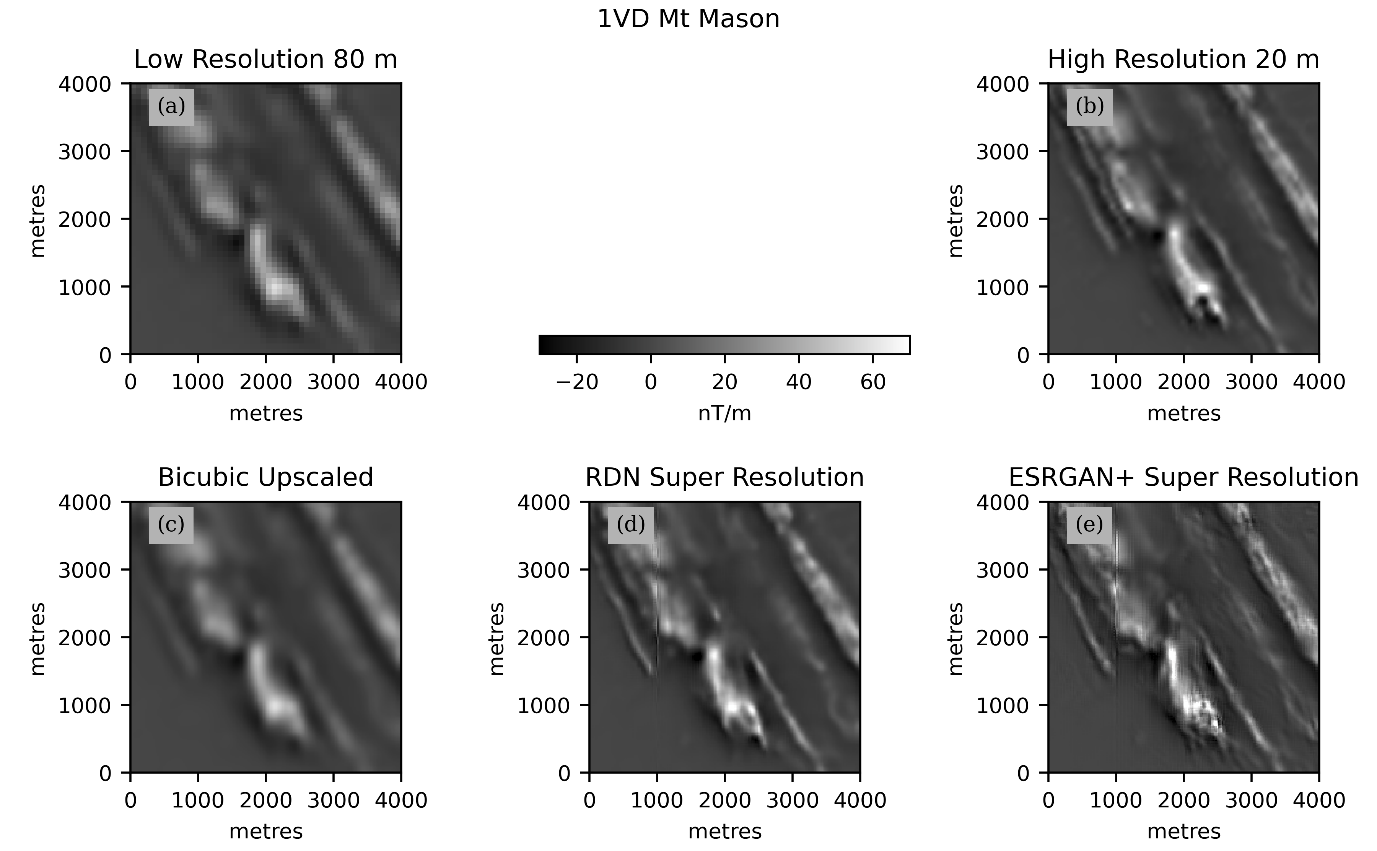
\includegraphics[width=\linewidth]{fig/p1/filtered.png}
    \caption[High Pass filtered results]{High Pass filtered test tile and its upsampled counterparts.
        The cut-off for the high pass Butterworth filter was selected with wavelength equal to the Nyquist wavelength of the LR grid, i.e.,\ four times the HR Nyquist wavelength
    }
    \label{fig:filtered}
\end{figure}

\begin{table}
    \begin{tblr}{
            colspec={
                    r
                    Q[si={table-format=2.3},r]
                    Q[si={table-format=2.3},l]
                    Q[si={table-format=2.3},r]
                    Q[si={table-format=2.3},l]
                    Q[si={table-format=2.3},r]
                    Q[si={table-format=2.3},l]
                },
            row{1-2} = {guard}
        }
                & Bicubic &           & RDN\textdaggerdbl{} &                 & ESRGAN+ &        \\
        \hline{}
                & Mean    & {Standard                                                            \\Deviation} & Mean & {Standard\\Deviation} & Mean & {Standard\\Deviation}                                                                         \\
        RMSE    & 13.545  & 26.576    & \textbf{7.265}      & \textbf{13.741} & 11.120  & 21.670 \\
        SISM    & 0.924   & 0.047     & \textbf{0.959}      & \textbf{0.037}  & 0.922   & 0.054  \\
        MS-SSIM & 0.971   & 0.018     & \textbf{0.988}      & \textbf{0.012}  & 0.976   & 0.020  \\
    \end{tblr}

    \caption[Accuracy Metrics]{Accuracy metrics for each upsampling method. The best performing method for each metric is bolded.}
    \label{tab:metrics}
\end{table}


\subsection{Jasper Hill / Lord Byron super-resolution}
A low-resolution TMI extent from the \qty{80}{\metre} state map over the Jasper Hill major resource project was selected for detailed investigation.
This extent was surveyed at \qty{50}{\metre} (optimal cell size of \qty{10}{\metre}), and is outside of both the defined training and test extents.
A zoomed result for each upsampling method is shown in \Cref{fig:jhilldykes}.
The bicubic filter produces a smooth interpolation with limited magnetic intensity enhancement of the features, while both neural network methods produce a more accurate value prediction.
East-West striking features, like those that have been associated with gold mineralisation in the region \parencite[p.~283]{salierTimingSourceGoldbearing2003} are better delineated when using RDN\textdaggerdbl{} and ESRGAN+, and nearly unobservable with bicubic interpolation.
This can be seen in the line profile (\Cref{fig:jhilldykes}, f), where a series of East-West striking features have a total magnitude of approximately \qty{100}nT in the low-resolution and bicubic grids, versus approximately \qty{200}nT in the Residual Dense Network prediction and HR groundtruth.
The ESRGAN+ prediction profile shows two distinct low TMI features, but they are poorly located and incoherent in the TMI grid (\Cref{fig:jhilldykes} e), which shows an example of the ripple-mark artefact previously noted.

\begin{figure}[hbt]
    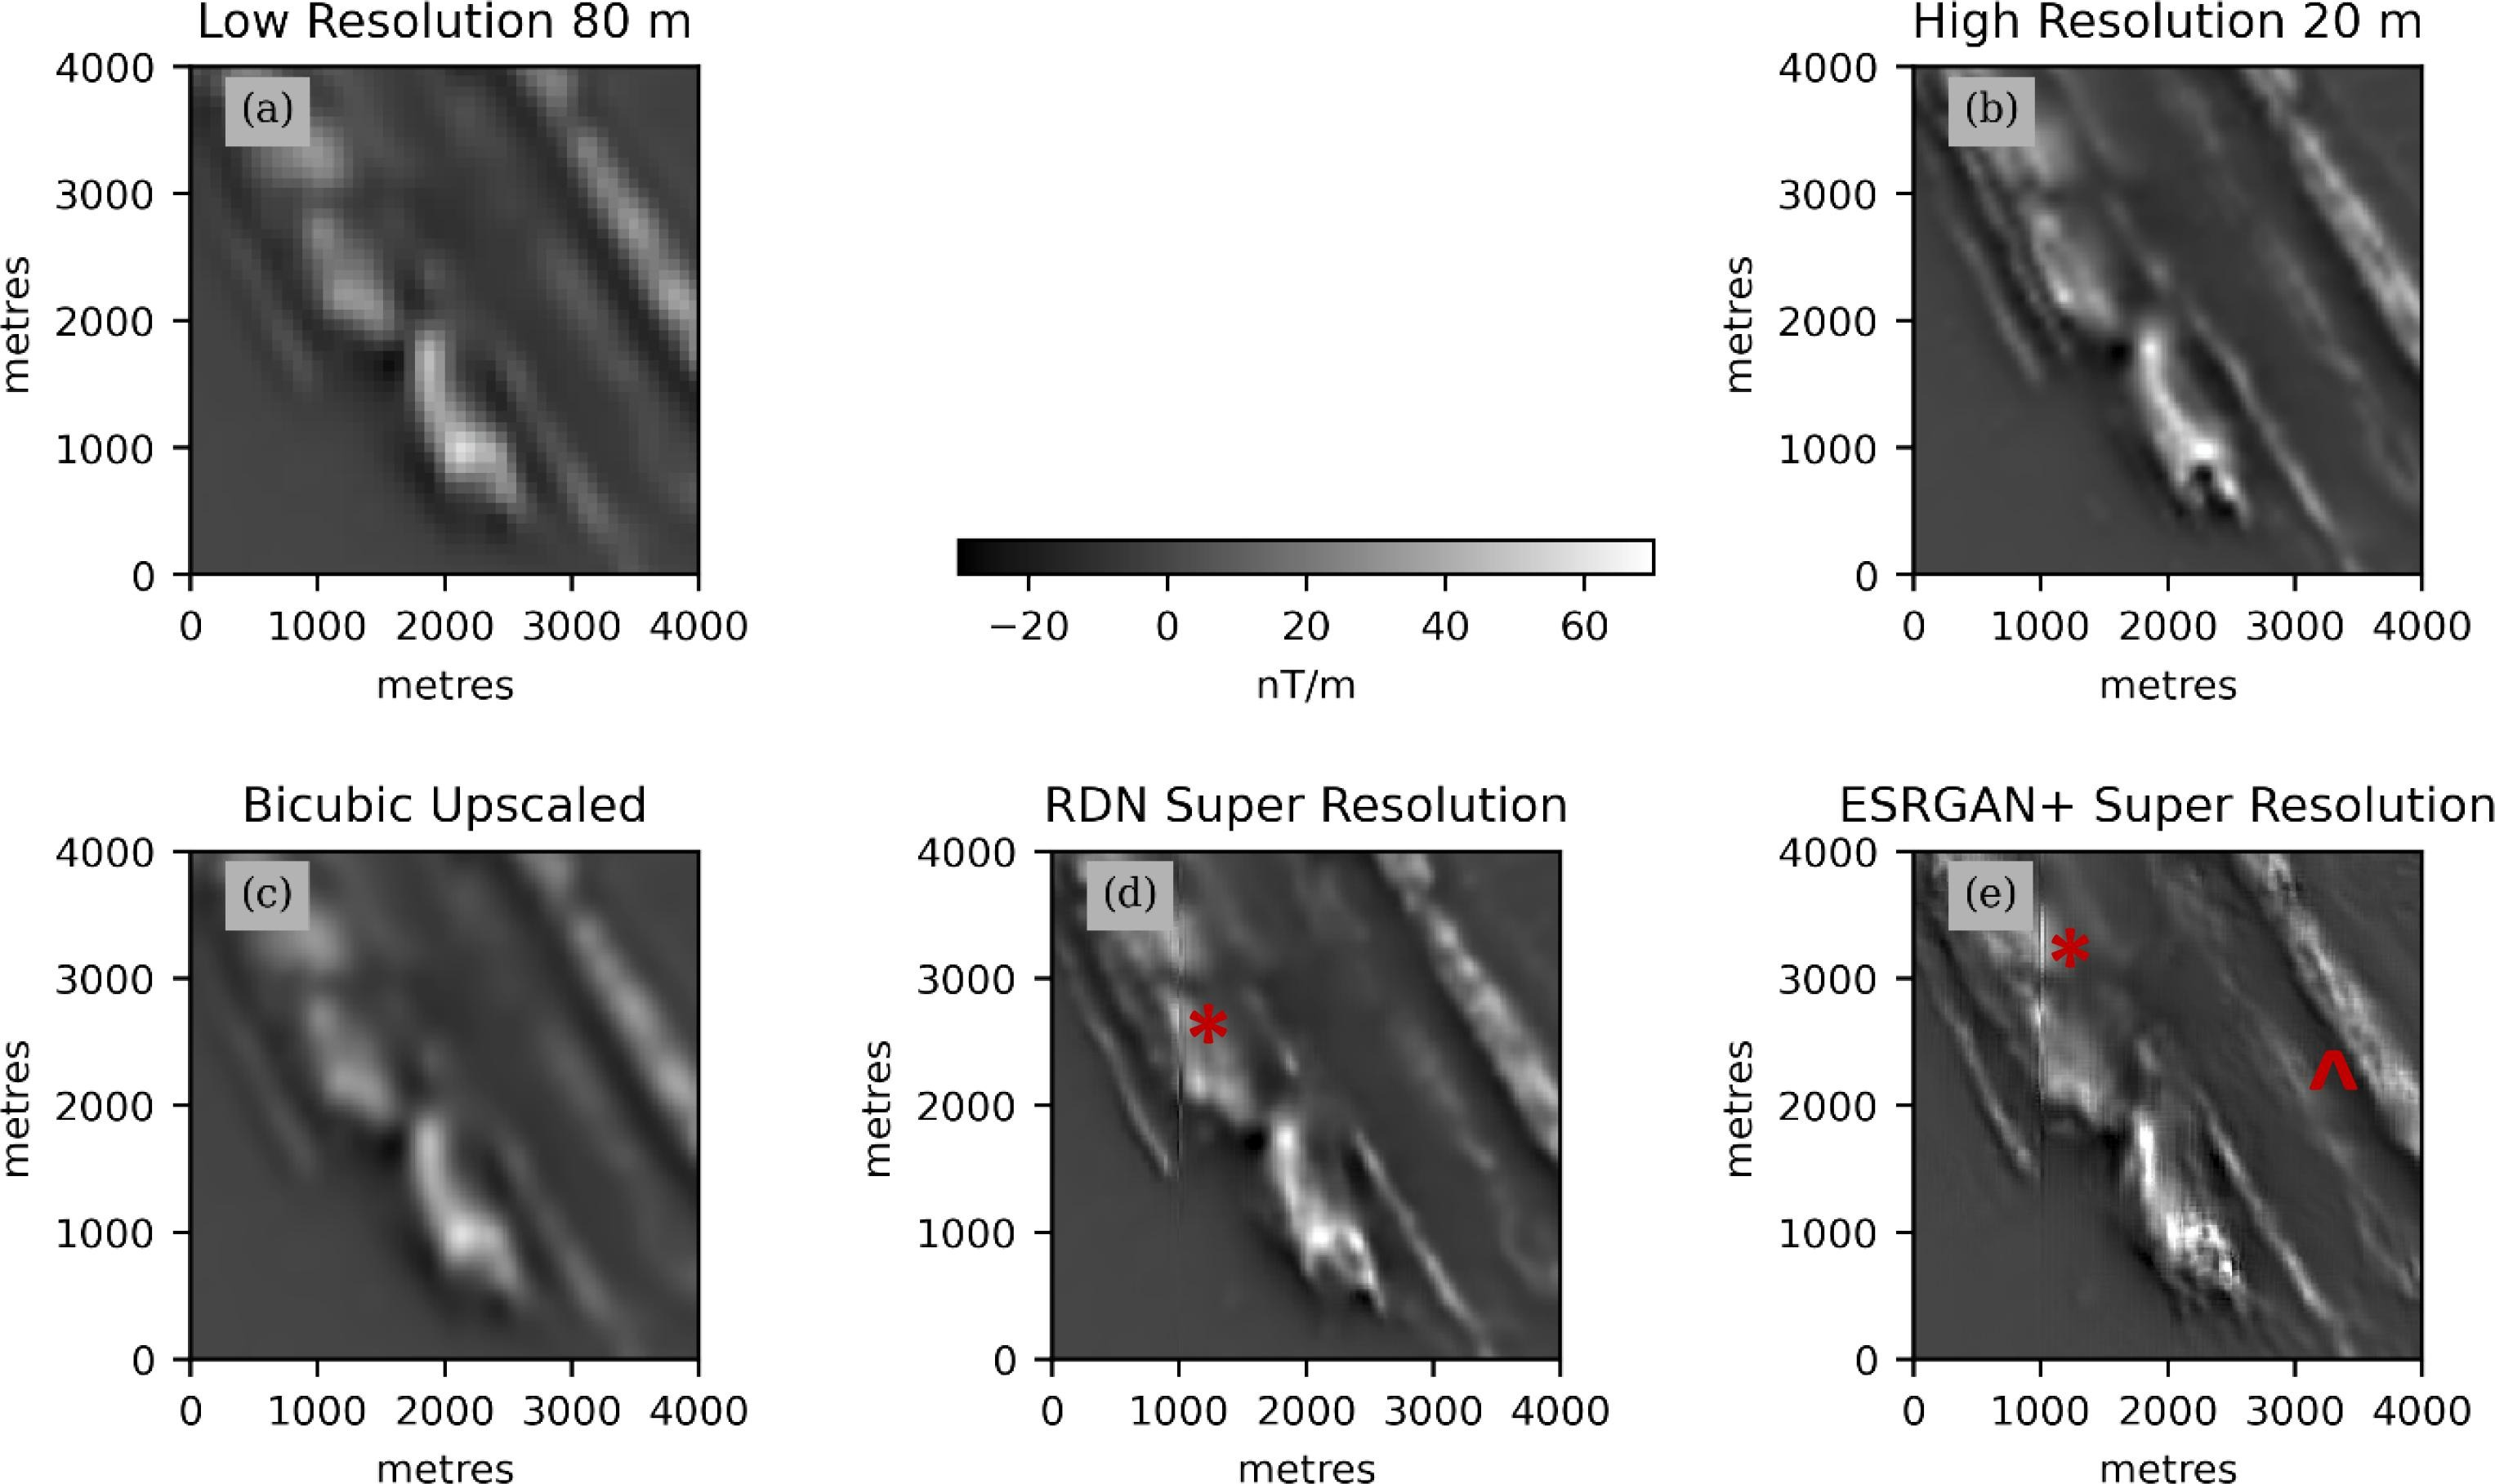
\includegraphics[width=\linewidth,trim={0 0 0 0},clip]{fig/p1/jhillvis.jpg}
    \caption[First Vertical Derivative SR TMI over the Mt Mason resource project]{First Vertical Derivative TMI over the Mt Mason resource project, with the super-resolution predictions (d, e) showing a variety of inference artefacts.
    Red asterisks (*) show a vertical tile boundary present as a 3--4 pixel-wide error in predicted TMI value.
    Red caret (\^{ }) indicates a region of subtle ripple-mark textural artefact, only present in ESRGAN+ predictions.
    }
    \label{fig:jhillvis}
\end{figure}

\begin{figure}[hbt]
    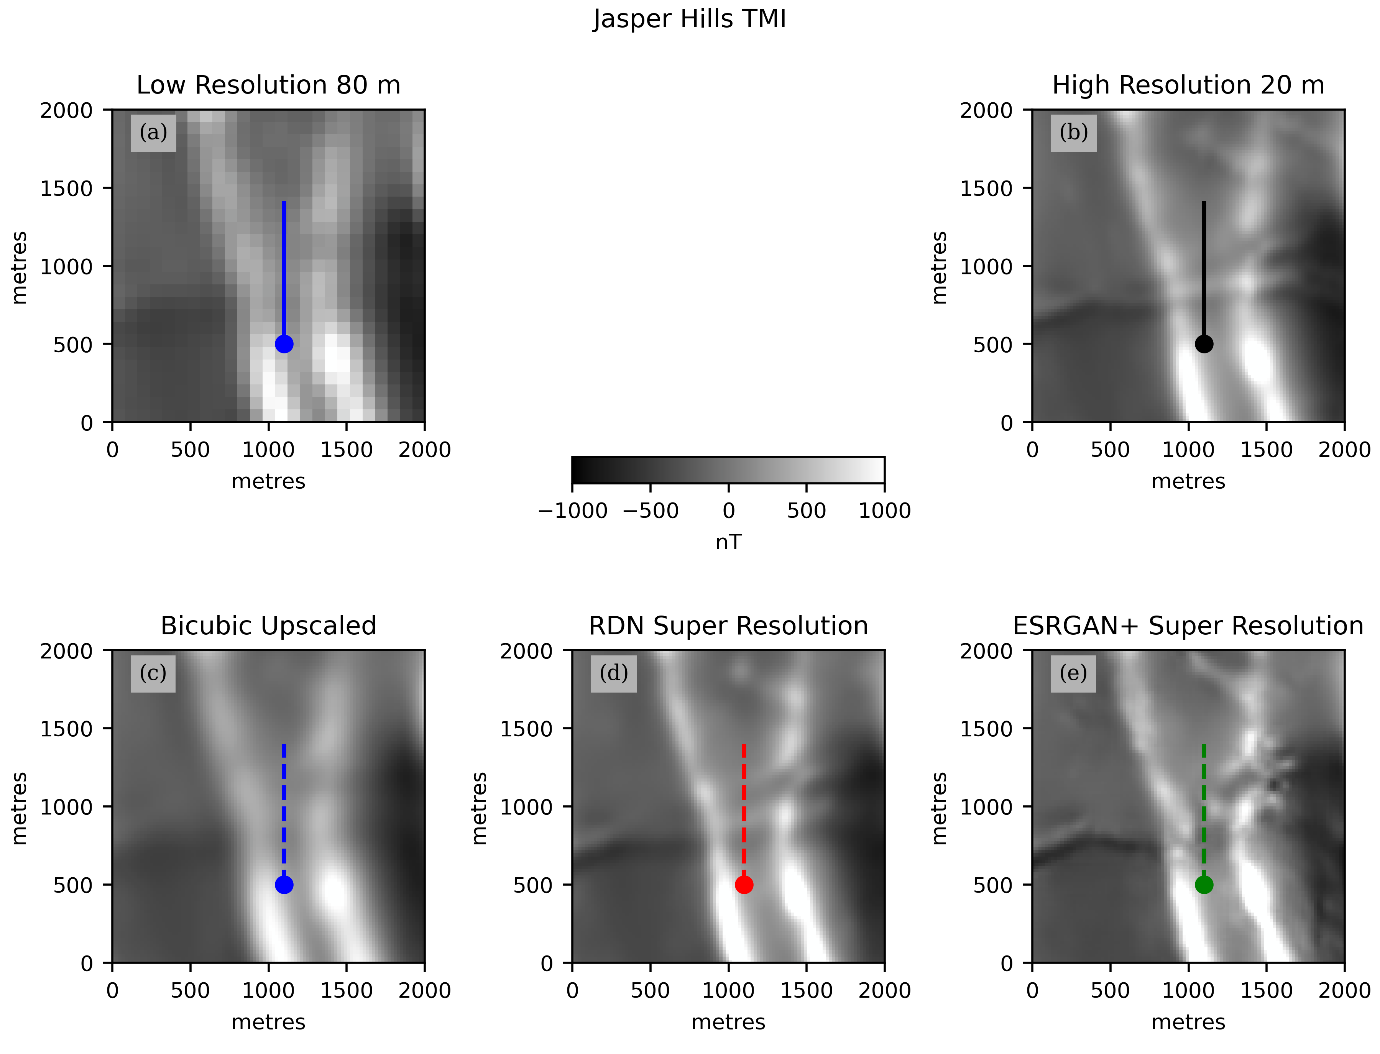
\includegraphics[width=\linewidth,trim={0 0 0 5mm},clip]{fig/p1/jhilldykes.png}
    \centering
    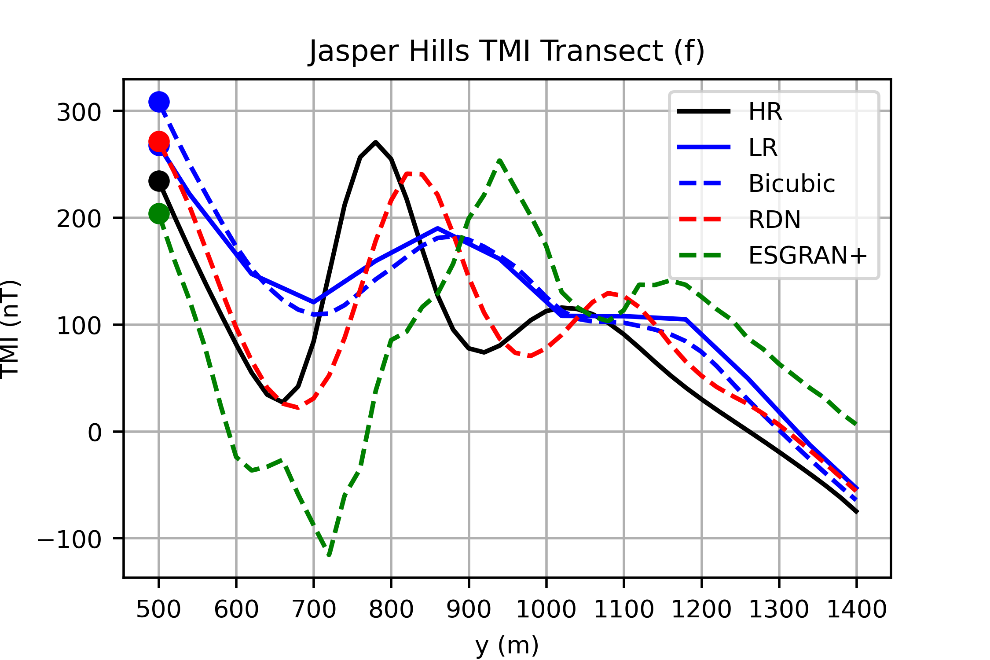
\includegraphics[width=0.7\linewidth]{fig/p1/transectp.png}
    \caption[Jasper Hills Project TMI grids and line profile]{Jasper Hills Project TMI grids (a--e) and line profile (f).
        Bicubic interpolation of the low-resolution grid closely matches the low-resolution grid, while both super-resolution methods better approximate the magnitude of the features present in the HR profile, between \qty{650}{\metre} and \qty{1020}{\metre}.
    }
    \label{fig:jhilldykes}
\end{figure}

\section{Discussion}
These results demonstrate that a neural network approach is suitable for high quality super-resolution of geophysics data, surpassing bicubic interpolation in each metric and better resolving structural features.
Importantly, mineralisation controlling structural features that are unresolvable in low-resolution grids become observable in super-resolved grids using a Residual Dense Network.
RDN\textdaggerdbl{} outperforms ESRGAN+ in both accuracy and structural metrics, and most closely visually matches the high resolution groundtruth.
However, ESRGAN+ occasionally appears to better reconstruct features present in the high-resolution ground truth when compared to RDN\textdaggerdbl{}, but at the cost of significant textural noise.
Based on this, RDN\textdaggerdbl{} shows the best performance for super-resolution CNN upsampling of magnetic grids, to assist in the interpretation of low-resolution grids.
The deep learning methods used here can be trained with data from other geospatial extents, either from scratch or by initialising the training with pre-existing model weights \parencite[][e.g.]{wangMineGANEffectiveKnowledge2020}.
The existing models can also be applied to other extents of \qty{80}{\metre} TMI grids without further training.
However, the training data used here are solely \qty{80}{\metre} TMI grids interpolated from high-resolution \qty{20}{\metre} state map extents in the southwest Eastern Goldfields Superterrane.
Magnetic anomalies and features that are dissimilar from those represented in the Superterrane (for example, different geological settings, or regions with different magnetic inclination) are likely to suffer from reduced performance.
This applies also to grids that do not have a cell size of \qty{80}{\metre}.
An example use case for either the method or trained models is super-resolving the Total Magnetic Intensity (TMI) Grid of Australia 2019 - seventh edition which is published by Geoscience Australia in only \qty{80}{\metre} and \qty{40}{\metre} cell size.
The trained \qty{80}{\metre} models in this work could be applied to the \qty{80}{\metre} TMI grid, or the method used with existing state map data to train a two times scale model to super-resolve the \qty{40}{\metre} grid to \qty{20}{\metre}.
Transferability of the model used in this study to other geological settings and magnetic inclinations requires further investigation, with the aim of developing a single multi-domain potential field upscaling model.

The use of the state magnetic map at \qty{80}{\metre} and \qty{20}{\metre} for training data serves as a ready-made analogue for a low pass filter process, which the super-resolution networks successfully learnt to reverse.
While the result presented here demonstrates the strong applicability of performing super-resolution with grids containing magnetic textures and features, it does not yet demonstrate a capability to super-resolve widely spaced line surveys as if they had been surveyed at closer line spacing.
Such grids include artefacts from the gridding process that do not occur in low pass filtered or interpolated high-resolution grids, and will present an additional challenge to super-resolve.
These challenges remain for future work.
Finally, the current models show good performance at a scale factor of \num{4}, which is a typically investigated scale factor in super-resolution research.
Provided with sufficient training data, super-resolution geophysics at other factors would be beneficial, especially targeting typical scale factors between regional and district-scale exploration surveys.

\section{Conclusions}
Convolutional neural network architectures, such as RDN and ESRGAN, are capable of super-resolution upsampling low-resolution magnetic grids into realistic high-resolution grids.
These super-resolved grids contain structural features and textural information that are accurate against ground truth high-resolution grids, that were otherwise unrecoverable through existing interpolation methods.
The method and existing trained models can be applied to other magnetic grid extents, in the Eastern Goldfields Superterrane and beyond.

% \section{Declaration of Competing Interest}
% The authors declare the following financial interests / personal relationships which may be considered as potential competing interests: This work was supported by a Rio Tinto Iron Ore PhD scholarship.

\printbibliography{}


\end{document}

\chapter{Super-resolution of Aeromagnetic Survey Data}
\label{ch:paper2}
% \newrefsection{}
% % \documentclass[manuscript.tex]{subfiles}
% \documentclass[12pt,a4paper]{report} %,openright,twoside
% \usepackage{thesisstyle}
% \addbibresource{bib/PhD.bib}
% % \setcounter{chapter}{2}
% \begin{document}

\title{Fine-tuning super-resolution for real-world aeromagnetic surveys}
\author[1*]{Luke Thomas Smith}
\author[1]{Tom Horrocks}
\author[1]{Eun-Jung Holden}
\author[1]{Daniel Wedge}
\author[2]{Naveed Akhtar}
\affil{Centre for Data-Driven Geoscience, School of Earth Sciences, The University of Western Australia (M006), 35 Stirling Highway, 6009 Perth, Australia}
\affil{Department of Computer Science and Software Engineering, The University of Western Australia (M002), 35 Stirling Highway, 6009 Perth, Australia}
\date{\today}
% \maketitle{}

\begin{abstract}
    Super-resolution is a contemporary deep learning technique to increase the resolution and high-frequency content of gridded data.
    However, despite the widespread success of super-resolution upscaling of natural photographs, its application to low-resolution geophysical surveys remains to be fully investigated.
    Previous applications to geophysical survey data generate training data pairs of low- and high-resolution grids by downsampling the high-resolution grid with standard image filters.
    These are a poor approximation to real-world low-resolution aeromagnetic grids constructed from sparsely sampled survey data.
    Moreover, the structural variation within the survey data depends entirely on the geological domain which is surveyed.
    The proposed super-resolution method uses realistic high-resolution and low-resolution pairs of gridded survey data, obtained by simulating aeromagnetic surveys of the data at close and wide line spacings.
    Additionally, transfer learning from synthetic data that represents a wide range of realistic geological domains is used to improve the generalisability of the resulting model.
    The structural accuracy of the method is improved using a secondary fine-tuning stage incorporating real-world survey data.
    The Local Texture Estimator neural network architecture is adapted for this task, and qualitative and quantitative measures of the super-resolution performance are reported.
    The results demonstrate that the proposed method is capable of transforming regional scale aeromagnetic surveys to high-resolution for a wide range of geological features.
\end{abstract}

\section{Introduction}
We propose a method for super-resolution (SR) upscaling of aeromagnetic geophysics data from diverse geological provenance.
This method uses transfer learning \parencite{tanSurveyDeepTransfer2018} from magnetic data forward modelled from a collection of synthetic geological models with realistic structures and petrophysical properties \parencite{jessellNoddyverseMassiveData2022}, and fine tuning with real-world data.
SR employed in this work leverages the contemporary Local Texture Estimator neural network \parencite{leeLocalTextureEstimator2022}, with a realistic method for sampling and gridding high- and low- resolution data.
The method is suitable for typical low-resolution regional aeromagnetic surveys in Australia.

\subsection{Resolution in geophysical data}
\label{sec:resinsurveys}
In exploration geophysics, the Earth's naturally occurring magnetic or gravitational potential fields can be used to survey the petrophysical expression of underlying geology.
These can be interpreted to inform geological mapping, resource modelling, and enhance the understanding of the subsurface.
Depending on the scale of investigation, surveys may be carried out from ground or airborne sensors.
Detailed ground-based surveys can be sampled at point spacings of tens of metres while avoiding local obstacles, but at a regional scale, aircraft are used to provide rapid and uniform coverage regardless of access constraints.
These airborne surveys collect data at wide line spacing to minimise cost, with lines in Western Australian low-resolution regional surveys typically \qty{400}{\m} apart, however, open access high-resolution surveys with line spacings of \qty{100}{\m} or closer are increasingly common.
Sampling along line is typically performed at \qty{10}{\Hz} or faster, which corresponds to several metres between samples at a nominal flight speed of \qty{70}{\m\per\s} \parencite{goodwinAirborneMagneticRadiometric2023}.
Because the power of shorter wavelengths in potential fields diminish with increasing distances from the source, aeromagnetic flights are flown as low as safety and topography permits.
Despite the use of precise navigation systems and skilled operators, these data are not collected in perfectly uniform lines at constant height, and the samples also contain noise components.

The subsequent analysis of surveyed potential fields generally relies on gridded data, and transforming irregularly distributed survey data to a regularised grids is the task of gridding.
There are several classes of gridding methods available.
Minimum Curvature gridding \parencite{briggsMachineContouringUsing1974} is routinely applied in industry applications, as it gives well characterised results in rapid time, with minimal manual intervention.
A comprehensive review of traditional spatial interpolation methods is presented by \textcite{liReviewComparativeStudies2011}.
Each method of gridding has characteristic interpolation traits (which when undesired are termed artefacts), but irrespective of the gridding process the detail resolvable in the output grid is a function of the sample height, sampling density, and the final cell size at which the grids are rendered.
Gridding at a finer cell size preserves higher frequencies present in the sampled data, resulting in greater detail.
This resolvable detail is termed resolution, and high-resolution better defines structures apparent in the data which are contextually important to interpretation.
When the cell size covers a quantified distance, the smallest resolvable detail can be expressed in terms of wavelength.
This is the grid's Nyquist wavelength, and is equal to twice the gridded cell size.
This corresponds to the widely known Nyquist frequency, i.e.\ the limit at which bandwidth-limited signals may be incorrectly resolved due to sampling below the Nyquist frequency, at half the sampling frequency.
For example, a potential field which lacks significant wavelength components shorter than \qty{200}{\m} will be adequately resolved by a grid with a cell size of \qty{100}{\m}, without spurious features known as aliasing.
Extending this concept, arbitrarily shrinking the cell size will not resolve additional detail unless also predicting features with wavelengths shorter than those present in the sample data.
These are limited by the sample spacing during acquisition.
% Low-resolution aeromagnetic survey data are the result of wide line spacings during acquisition, with the resulting grid cells predominantly being those predicted by interpolation between sparse sample points.
Achieving higher resolution traditionally requires additional sampling to increase the grid resolution. %, which refines structures in the response and reduces blocky textures and other gridding artefacts.
In addition to human interpretation, machine processing of geophysical data is benefitted by using higher resolution data, with the negligible cost of increased computational load.

A small number of regions in Western Australia are covered by high-resolution aeromagnetic surveys with a line spacing of 100 m or closer, and these are biased toward prospective geological terranes \parencite{howardAirborneGeophysicalCoverage2004}.
Therefore, example-based learning methods trained using these aeromagnetic data will be biased for performance in these domains, while lacking in those that have been so far regarded as unprospective.
Addressing costly data acquisition, common in geoscience \parencite{dawsonImpactDatasetSize2023}, can be done by transfer learning.
This assists example-based methods by initially using a larger source dataset which shares properties with the target dataset.

In order to improve the generalisation of an example-based neural network for regions without high-resolution coverage, we propose using transfer learning \parencite{tanSurveyDeepTransfer2018} to fine-tune a synthetic data baseline model with high-resolution, real-world survey grid data.
The synthetic geophysical data \parencite{jessellNoddyverseMassiveData2022} are forward modelled from 3D petrographic voxel models with varied geological histories.
These provide a diverse set of features, but these lack truly realistic characteristics, such as high frequency near-surface magnetisation, and features from complex geological processes such as metasomatism or remnant magnetisation.

Thus, two approaches are made in this study to address the challenges of training an example-based model with limited suitable geophysical data.
Firstly, to make use of geologically diverse synthetic data, with a realistic sampling and gridding method to generate low-resolution data for training.
Secondly, to fine-tune this model using real-world grid data prepared with the same sampling method.

\subsection{Prior work}
Numerically, image interpolation can be done using interpolating functions, such as splines \parencite{keysCubicConvolutionInterpolation1981}, kriging \parencite{hansenInterpretiveGriddingAnisotropic1993} or other methods.
These methods are limited in their performance by the quality of their neighbouring observed values, and their distance.
Deep learning methods similarly use their spatial neighbours, but do so in the context of trainable filters, and across larger extents of the input.
In this way, deep learning super-resolution models are supported by latent information retained from the training dataset, in addition to information contained within the input being upscaled.

Instead of increasing the sampling density, the detail in potential field grids can be enhanced by calculating the potential as if it were sampled at a smaller source-sensor distance, in a process known as downward continuation \parencite{bullardDeterminationMassesNecessary1948}.
At large source-sensor distances, high frequencies are diminished below the noise floor to the point of unobservability, resulting in grids that show only broad scale features, typically representing spatially extensive features deep in the crust.
Downward continuation can be performed with the grid representation of the field, or by modelling causative sources and forward modelling the response at another height \parencite{pilkingtonPotentialFieldContinuation2017}.
In either approach, it is common for noise in the sampled grid product to be significantly increased in the downward continued product, limiting the useful vertical continuation extent of of the method to six times the cell size \parencite{dampneyEquivalentSourceTechnique1969,zuoDownwardContinuationTransformation2020}.
Resolution enhancement through neural network approaches to downward continuation \parencite{liStableDownwardContinuation2023,yeHighprecisionDownwardContinuation2022} is a promising research direction in super-resolution geophysics, but the training data are distinct.
The proposed line-spacing based methods use data prepared using high- and low-resolution survey designs, while neural network continuation approaches prepare data using the above numerical continuation methods.

Recently, aeromagnetic resolution enhancement has been performed with deep learning SR \parencite{bavandsavadkoohiHighresolutionAeromagneticMap2023,smithMagneticGridResolution2022}.
The method of \textcite{smithMagneticGridResolution2022} is presented in \Cref{ch:paper1} of this thesis.
These two approaches operate on regional aeromagnetic data at four times scale, using variants of the SRGAN convolutional neural network originally by \textcite{ledigPhotorealisticSingleImage2017}.
The method of \textcite{smithMagneticGridResolution2022} demonstated SR methods are capable of upsampling low-resolution magnetic textures and predicting accurate short wavelengths for these data.
Comparison was made against numerical filters such as the bicubic filter.
However, the low-resolution data were created using a polynomial filter that suppressed high frequencies, rather than a real-world low-resolution geophysical sampling process.
The method of \textcite{bavandsavadkoohiHighresolutionAeromagneticMap2023} uses low- and high-resolution aeromagnetic data from regional surveys in Quebec, Canada, with a realistic low-resolution transform from line spacing and sample altitude differences.
% The dataset contains \qty{267} sample grids from surveys in Quebec, Canada, prepared from surveys with a low-resolution line spacing of \qty{800}{\m}.
The proposed method is distinct from these prior works with its use of extensive and geologically varied synthetic data in coordination with real survey data to improve generalisation for regional aeromagnetics in Australia, and the use of a modern MLP-based SR network.

Deep learning techniques for SR typically use paired high- and low-resolution image data, with the objective to learn the transform from low resolution to high.
This is an ill posed challenge, because many high-resolution images share the same low-resolution representation \parencite{dongImageSuperresolutionUsing2016}.
For photographs and natural image rasters with large representative training corpuses available, such as ImageNet \parencite{dengImageNetLargescaleHierarchical2009} and DIV2K \parencite{agustssonNTIRE2017Challenge2017}, SR methods have progressed to the point that high quality enhancement at four times scale is readily accessible to end-users \parencite[e.g.][]{wangRealESRGANTrainingRealWorld2021}.
The performance of SR for photographs and digital images has been intensely explored \parencite[see a review in][]{moserHitchhikerGuideSuperResolution2023}.
Prior work specific to this study are reviewed in \Cref{sec:2nnsr}.

Photographs and other natural images of interest to computer vision are typically created by capturing light from an image sensor or are explicitly mapped on a grid using a raster graphics program.
In these rasters each pixel is regularly distributed and the resolution is a factor of the pixel density of the sampling sensor or the software defined grid.
These data are encoded to regular arrays of pixel values, commonly as three-channel rasters representing the red, green, and blue intensities of each pixel.
For natural images, a common approach to generating low-resolution data is to interpolate the high-resolution image to a smaller size using a transform such as bicubic downsampling.
Aerogeophysical grids are distinct from these image rasters due to the potential field sampling and grid interpolation process outlined in \Cref{sec:resinsurveys}, and the extent to which widely spaced low-resolution geophysical line data can be enhanced, and characteristics of the resulting super-resolved grids remain to be fully explored.
Most critically, aeromagnetic data are highly sampled in the direction of flight lines but are under-sampled in the line-perpendicular direction.
The resulting grid rasters may have isotropic cell size, but the frequency content in each axis is anisotropic, being a factor of the sampling frequency in the line-perpendicular (low) and line-parallel (high) directions.
Being sampled as a single component of the vector potential field, these data contain a single channel, and the data contain multiple sources of noise components.
Furthermore, the features present in these data are dependent on the subsurface geology, varying between smooth domains without significant near-surface magnetisation, through to highly deformed igneous stratigraphic units with complex high-intensity structures.
The recorded intensity values have high dynamic range, spanning tens of thousands of nanotesla, while contextually important features may be defined by tens of nanotesla \parencite{kovesiPhasePreservingTone2012}.
Because of these differences, pre-existing super-resolution models trained on large image corpuses are not suitable for predicting higher frequency signals in geophysical grids.

We propose a method that simulates the line sampling of both synthetic and real data, thereby more closely reflecting real-world low-resolution aeromagnetic data, at scales typical of those in exploration in Australia.

\subsection{Neural network super-resolution}
\label{sec:2nnsr}
Deep learning super-resolution (SR) is the task of predicting interpolating values to resolve rasters with a higher resolution, and has been predominantly performed in the domain of Convolutional Neural Networks (CNN) following the success of SRCNN \parencite{dongLearningDeepConvolutional2014}.
Recently, multi-layer perceptrons (MLPs) have become a state-of-the-art alternative for SR\@.
In an MLP (also known as a fully connected network), all neurons in a given layer are connected to all neurons in the immediately adjacent layers.
This contrasts with CNNs, where spatially related neurons are sparsely connected between layers via a convolutional kernel.
Fully connected MLP networks have been described for several decades, however, networks partly or entirely comprising fully connected layers saw little interest for SR following the success of SRCNN \parencite{dongLearningDeepConvolutional2014}.
It was noted in \parencite{arjovskyWassersteinGAN2017} that MLP networks were known to be a poor backbone in generative adversarial networks, an architecture which was seeing wide application in contemporaneous computer vision tasks.
One early SR network featuring fully connected layers was for multi-frame video super-resolution \parencite{chengFastVideoSuperresolution2012}, while another was used to investigate depth images \parencite{chenSingleDepthImage2018}.
\Textcite{tanFeatureSuperResolutionMake2018} aimed to create high-resolution feature maps for machine interpretation rather than subsequent visual observation.
Among the first image SR networks incorporating an MLP for human perception was by \parencite{tangDeepResidualNetworks2020}, who replace convolution operations in their network's final image reconstruction with a fully connected layer.
They suggest a fully connected layer outperforms convolutions for image reconstruction due to the wider receptive field of the MLP\@.

An implicit function aims to learn a specific function and parameterise it within a neural network model.
In an image or geophysical grid context, the function may map grid coordinates to the value at those coordinates.
While extensively developed for point cloud and other 3D data \parencite[e.g.][]{jiangLocalImplicitGrid2020} there have been numerous examples for super-resolution.
These include SIREN \parencite{sitzmann2019siren}, LIIF \parencite{chenLearningContinuousImage2021}, and LTE \parencite{leeLocalTextureEstimator2022}.
Notably in these networks, the learned function has continuous domain, despite the discretised grid input.
Super-resolution can be achieved by sampling the learned function at any arbitrary grid cell size smaller than the original input \parencite{chenLearningContinuousImage2021}.
While a stand-alone MLP such as SIREN is capable of parameterising a single function, when used in an autoencoder framework (such as with LIIF or LTE), an arbitrary input can be encoded, upscaled, and subsequently reconstructed using fully connected layers \Cref{fig:ltenet}.
An autoencoder approach generalises MLP based super-resolution to any image or grid not seen in the training set.

The local texture estimator (LTE) of \parencite{leeLocalTextureEstimator2022} is adapted for this work due to its performance in the task of image super-resolution.
The encoder in LTE can use the feature extraction capability of traditional SR CNNs such as EDSR \parencite{limEnhancedDeepResidual2017} or RDN \parencite{zhangResidualDenseNetwork2018}, or a SwinIR \parencite{liangSwinIRImageRestoration2021} transformer-based encoder.
In the original implementation of the SR CNN networks, the extracted image features are upsampled and returned to the image domain by convolutional layers.
In LTE, the latent extracted features are further processed by the LTE network component before reconstruction to image space by an MLP\@.
An overview of the structure of the LTE network is shown in \Cref{fig:ltenet}.
Specifics of the LTE implementation to investigate the performance of SR for geophysical grids from a range of geological domains are detailed in \Cref{sec:2lte}.

\begin{figure}[hbtp]
    \centering
    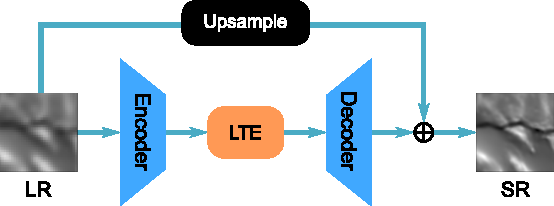
\includegraphics[width=0.75\linewidth]{fig/p2/ltenet.pdf}
    \caption[The LTE architecture]{
        The LTE super-resolution network is structured as an autoencoder.
        The encoder can take the form of RDN (prior the upsampling and reconstruction, see \Cref{fig:rdn}), or transformer-based networks.
        The decoder is an MLP network, and is used for image reconstruction.
        A long-range skip connection with nearest neighbour upsampling allows low-resolution features, common to both LR and the HR target, to bypass the network.
        The LTE network block performs high-resolution upscaling of extracted features in the frequency domain.
        Simplified from \textcite{leeLocalTextureEstimator2022}, where the LTE block is further detailed.
    }
    \label{fig:ltenet}
\end{figure}

The remainder of this paper is structured as follows.
\Cref{sec:2methods} describes the experimental design to generate low-resolution aeromagnetic survey grids from synthetic and real-world data, where \Cref{sec:baseline,sec:finetune} specifically describe the training approach for the neural network model.
Results are presented in \Cref{sec:2results} and are discussed in \Cref{sec:2discussion}.
Conclusions are drawn in \Cref{sec:2conclusion}.

\section{Data and experimental methods}
\label{sec:2methods}
A realistic geophysical low-resolution transform is developed by simulating aeromagnetic sampling of high-resolution survey grid datasets, and re-gridding the resulting samples.
The proposed dataset methodology uses synthetic forward modelled potential field data to train a selected performant super-resolution network, and the resulting baseline model is subsequently used for transfer learning to fine-tune train the model with real aeromagnetic survey grid data.
The performance of the method is qualitatively described on real survey grid extents, and quantitatively described with image quality metrics.

\subsection{Synthetic potential fields}
A novel synthetic dataset is used to train and validate the initial model.
This is based on the Noddyverse \parencite{jessellNoddyverseMassiveData2022}, a suite of one million geologically realistic petrophysical voxel models with accompanying forward modelled geophysics.
The block models are constructed as a sequence of realistic geological histories with an initial stratigraphy and tilt, followed by three randomly selected deformation events of fold, fault, unconformity, dyke, plug, shear-zone, or tilt.
Each model in the suite records the parameters of the deformation history, the complete final 3D subsurface geology voxel model with associated petrophysics, and final forward models of the magnetic and gravity potential fields.
All data are modelled at \qty{20}{\m} spacing in each direction for \qty{4000}{\m} (\qty{200} cells) in each axis, and the potential field forward models are calculated at \qty{100}{\m} above the flat model surface.
Only the magnetic forward model is used in this work.

Included in the published dataset \parencite{jessellNoddyverseMassiveData2022} are a complete list of all models, and a separate list comprising a randomly selected subset of \qty{10000} models.
The first \qty{960000} models from the full list are used for training, and the last \qty{8000} models are used for validation.
In both cases, this excludes models present in the list of \qty{10000} models, which are reserved as a test data set.
The \numproduct{200 x 200} cell forward models are cropped to \numproduct{180 x 180} cells, subsequently referred to as the ground truth (GT) models.

\subsection{Simulated surveys}
\label{sec:simsurveys}
To simulate the acquisition of aeromagnetic data, the \qtyproduct{20 x 20}{\m} total magnetic intensity (TMI) forward models are line sampled at a factor of \(4n\)  (i.e., \(4n \times 20\) m sampling in \(x\), \(1 \times 20\) m sampling in \(y\)).
The line direction is nominally ``North-South'' such that entire array columns are sampled or unsampled.

The \(n = 1\) case is the high-resolution target (HR) with every fourth line of GT sampled at a nominal line spacing of \qty{80}{\m}, similar to real-world regional high-resolution airborne geophysical surveys.
These sampled line data are gridded at a cell size of \qty{20}{\m} using the cubic method from Verde \parencite{uieda2018}, which is one quarter of the line spacing, following the convention of \textcite{reidAeromagneticSurveyDesign1980}.
It is important to note that while the HR grid has a cell size of \qty{20}{\m}, it is not equivalent to the \qty{20}{\m} cell size GT grid, because unsampled cells are interpolated during the gridding process.
The result is a loss of high frequency detail in the line-perpendicular direction, as well as the loss of features present only in the unsampled lines.

The low-resolution input data (LR) are sampled from GT at \(n = 4\).
At this scale the LR line spacing is \qty{320}{\m}, the cell size is \qty{80}{\m}, and the array shape is \numproduct{45 x 45} cells, covering the same extent as HR\@.
Subsampling and gridding of the pre-generated Noddyverse data is performed on-the-fly during training.
The cubic method of Verde (itself implemented by Scipy Clough-Tocher 2D interpolation \parencite{2020SciPy-NMeth}) produces a \(C^1\) smooth grid with minimised curvature.
This type of gridding is common for regularising geophysical data and creates a variety of typical low-resolution artefacts such as aliasing and bullseye artefacts.
\Cref{fig:lrdata} shows an example of the resulting high- and low-resolution grids for the proposed line sampling and gridding process.

This method of generating low-resolution training data is distinct from computer-vision image super-resolution, where a three-channel colour image is downsampled using an interpolating filter such as nearest neighbour or cubic splines operating on all pixels in the original image.
It is also distinct from previous geophysical deep-learning super-resolution work \parencite{smithMagneticGridResolution2022} where the raster data used are extracts from regional compilation TMI maps, created using a third order Newton polynomial filter, similar in effect to cubic spline interpolation.
The downsampling method used here is representative of low-resolution airborne sampling and subsequent gridding processes in real world geophysics.

The distribution of magnetic anomaly values within both the magnetic merged grid of Western Australia and the Noddyverse dataset is unimodal and centred near \qty{0}{\nano\tesla}, with a standard deviation of approximately \qty{500}{\nano\tesla}.
Despite this, the HR and LR grids are clipped between \qty{-10000} and \qty{10000}{\nano\tesla}, then min-max normalised to the range 0 to 1.
This wide clipping range is selected to ensure adequate reconstruction of structures with high magnitude intensities, which are important to geological interpretation.
Any predictions made outside of this range during inference are also clipped.

\Cref{fig:lrdata} presents data generated with the proposed low-resolution transform for a range of geological histories.
\Cref{fig:lrdata}(a, b, c) shows a synthetic tile with the geological history ``stratigraphy, tilt, fold, tilt, fold''.
The forward model contains a long-wavelength linear magnetic structure, and a sharply defined high intensity magnetic unit.
The high frequencies required to define the second feature are not captured by the LR grid sampling, resulting in aliasing.
\Cref{fig:lrdata}(d, e, f) is recorded with a geological history of ``stratigraphy, tilt, fold, fold, fold'', and presents two folded negative anomalies that converge to the south.
Insufficient sampling in the LR grid causes the spatial relation to be incorrectly interpreted as converging in the centre of the figure, which may be interpreted differently than in the target high-resolution grid.

\begin{figure}[hbtp!]
    \centering
    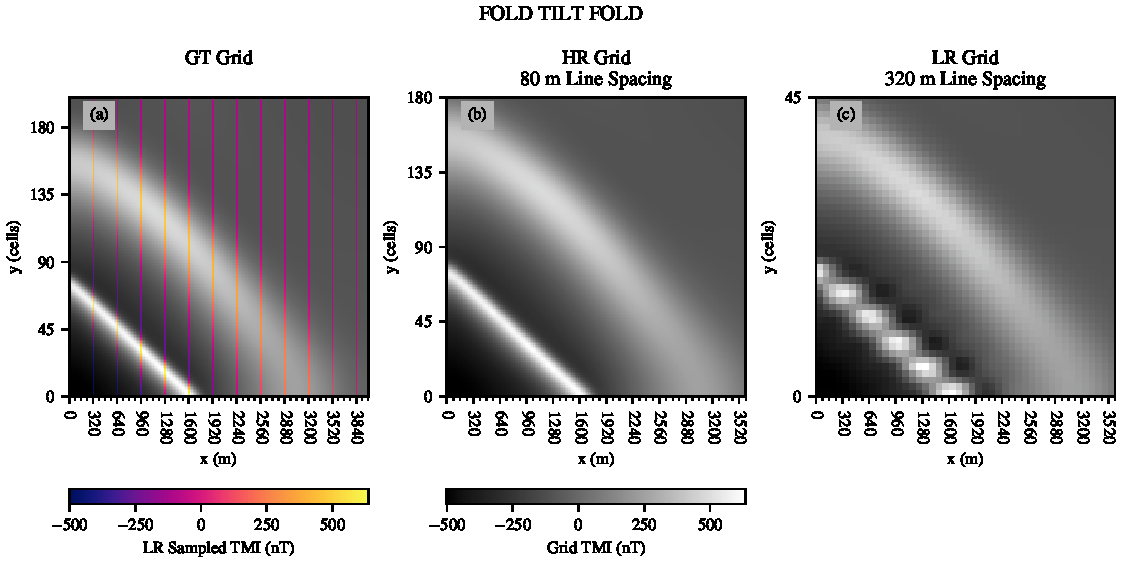
\includegraphics[width=\linewidth,trim={0 0 0 5mm},clip]{fig/p2/inp_data_Noddy_169.pdf}
    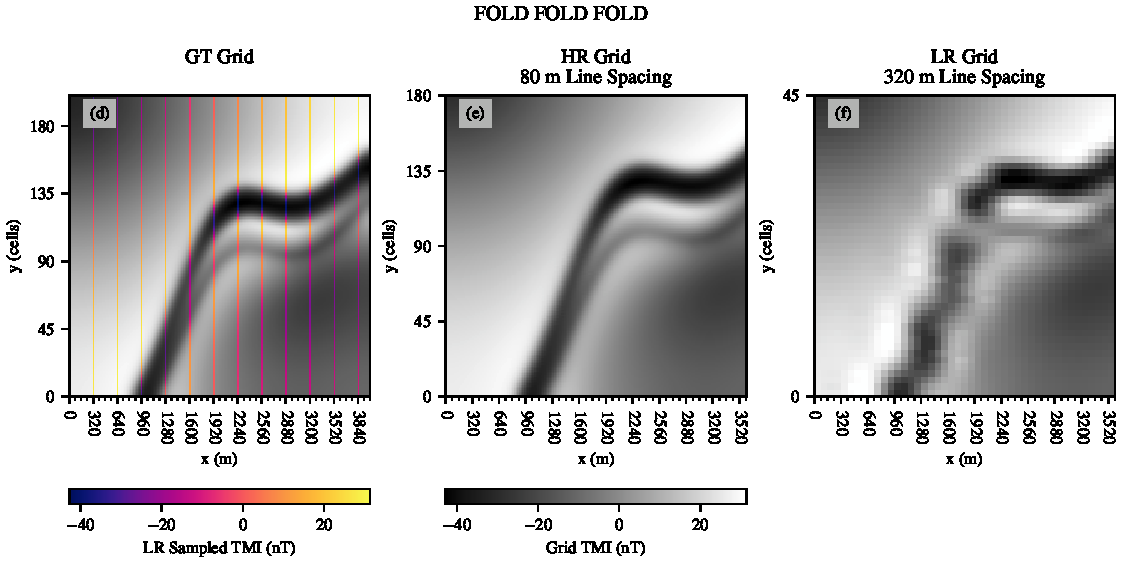
\includegraphics[width=\linewidth,trim={0 0 0 5mm},clip]{fig/p2/inp_data_Noddy_165.pdf}
    \caption[Low-resolution geophysics grids]{
        The result of the proposed sampling and gridding on a two synthetic tiles loaded from the collection of \textcite{jessellNoddyverseMassiveData2022} at 4x scale.
        Note the coloured lines and accompanying major tick marks in the ground-truth grid (GT a., d.,) indicate cells which are sampled and used for gridding in the low-resolution grid (LR c., and f.,).
        High-resolution (HR b., e.,) is sampled and gridded from GT, with survey lines indicated by minor tick marks.
        The minimum curvature gridding process results creates a variety of low-resolution degradations.
    }
    \label{fig:lrdata}
\end{figure}
%TODO

\subsection{Baseline training with synthetic data}
\label{sec:baseline}
While each of the models in the synthetic training dataset have unique petrophysical parameters, there are only \qty{343} distinct sequences of deformation events.
This leads to feature similarities between many samples within the dataset, varying in rotation, scale, locality, and magnitude.
For this reason, augmentation is unnecessary, and the line sampling direction is kept nominally north-south.
Due to this similarity and the \qty{960000} samples used from the Noddyverse dataset, only one epoch is used.
The batch size is set to 8. The Adam optimiser is used with an initial learning rate of \num{0.0001}, and this is successively halved at 50\%, 70\%, and 90\% of the overall training progress.
Training was undertaken on a Nvidia RTX 3090 with \qty{24}{\giga\byte} of VRAM, in an Intel i9-10900KF workstation with \qty{64}{\giga\byte} of RAM\@.
The duration for the single epoch was approximately \qty{10}{\hour}.

%TODO

\subsection{Fine-tuning with aeromagnetic survey data}
\label{sec:finetune}
To improve the performance of the model on real world geophysical data, the synthetic-trained model is subsequently trained on data re-gridded from the \qty{20}{\m} magnetic merged grid of Western Australia 2020 \parencite{brett20MagneticMerged2020}.
These data are selected from extents of the state grid where surveys were performed at \qty{100}{\m} line spacing or closer, which when gridded at \qty{20}{\m} cell size, support the same Nyquist wavelength as the \qty{20}{\m} cell size of the Noddyverse dataset.
Small holes and gaps in overlapping survey coverage were closed to ensure sufficient contiguous coverage.
These data are initially extracted as approximately \num{10000} “ground truth” patches of \numproduct{200 x 200} cells at \qty{20}{\m} cell size, equivalent to the synthetic dataset.
High- and low-resolution training pairs are created from these data using the same line sampling process as described in \Cref{sec:simsurveys}.
Due to the smaller number of patches, these data are augmented during training.
The first augmentation is extracting three additional sets of repeat patches, offset in both directions by 53, 107, and 150 cells.
The geological features present in these offset patches are shifted compared to the original, and entirely different cells are subsampled in each offset.
Across all four sets of offsets, there are \num{37726} unique samples.
The second augmentation is a randomly applied 90-degree rotation of the ground-truth grid prior subsampling and gridding, resulting in grid data with features that are sampled perpendicular to the unaugmented lines.
The remaining augmentations are each randomly applied with \qty{50}{\percent} chance, and are flips and 90-degree rotations of the high- and low- resolution grids after gridding.

Training the real survey model is performed after loading initial weights from the synthetic-trained baseline model.
All hyperparameters remain identical to those used for synthetic baseline training, including the learning rate schedule and initial rate of \num{0.0001}.
Because of the smaller dataset and use of augmentations, \num{10} epochs were used, increasing the training duration by approximately one hour.


\subsection{Network selection}
\label{sec:2lte}
LTE \parencite{leeLocalTextureEstimator2022} is implemented to super-resolve synthetic and real potential field geophysical data with low resolution resulting from line spacing.
The LTE component of the LTE network transforms the encoded latent features to frequency and amplitude features using trainable convolutions.
Both the amplitude and frequency features are then upsampled using nearest neighbour filter interpolation.
The frequency components are combined with phase information, which is extracted from the input by an additional MLP, and the resulting features are passed through a sinusoidal activation function before being combined with the amplitude features.
Finally, the decoding MLP restores these frequency domain features to the spatial image domain.
To precondition the network for learning high-resolution features, a long-range skip connection with simple upscaling passes low-resolution content common between the upsampled LR and the HR target to the output of the MLP\@.
Because TMI data are single channel, the input and output channel count are set to one.
The SwinIR encoder implementation by is used, and the MLP decoder retains the same configuration as the authors \parencite{leeLocalTextureEstimator2022}.

\section{Results}
\label{sec:2results}
Due to the variable dynamic range of magnetic anomaly grids and the relative importance of structural accuracy for gridded data, image quality assessment methods typically used for RGB images such as peak signal-to-noise ratio or mean-squared error are an inadequate quantitative measure of upscaling performance for geophysics.
FSIM \parencite{linzhangFSIMFeatureSimilarity2011} is a full reference image similarity metric that quantifies structural similarity, rather than individual cell values.
% FSIM is used to quantify the quality of the super-resolved image.
%TODO complain about SSIM Structural Similarity (SIM) \parencite{wangImageQualityAssessment2004}
Model performance is quantified using FSIM in \Cref{tab:2metrics}, with increasing similarity causing the metric to approach 1.0.
It is seen that fine-tune training increases FSIM score for the task of super-resolution for aeromagnetic grids, over the baseline model.

\begin{table}[hbtp]
    \begin{tblr}{
            colspec={
                    r |
                    Q[si={table-format=2.3},r]
                    Q[si={table-format=2.3},l] |
                    Q[si={table-format=2.3},r]
                    Q[si={table-format=2.3},l]
                },
            row{1} = {guard}
        }
                         & \SetCell[c=2]{c} Reserved synthetic test &              & \SetCell[c=2]{c} Aeromagnetic grid dataset                \\
        \hline{}
                         & \(\mu{}\)                                & \(\sigma{}\) & \(\mu{}\)                                  & \(\sigma{}\) \\
        Baseline model   & 0.9844                                   & 0.0296       & 0.9731                                     & 0.0086       \\
        Fine-tuned model & 0.9838                                   & 0.0329       & 0.9754                                     & 0.0078       \\
    \end{tblr}

    \caption[Accuracy Metrics]{Mean (\(\mu{}\)) and standard deviation (\(\sigma{}\)) of the FSIM metric for each upsampling method, for each test set.
    While the performance of the fine-tuned model is lower on synthetic data, the performance on real-world aeromagnetic grids is increased.}
    \label{tab:2metrics}
\end{table}

Qualitative results are shown to provide examples of structural improvement when using the fine-tuned model trained with open access survey data, compared to the baseline model trained with synthetic data.

\Cref{fig:srdata23,fig:srdata14,fig:srdata17,fig:srdata18} contain open access grid data from the Eastern Goldfields Superterrane of Western Australia, prepared using the proposed method.
Each figure follows the following layout for the grids.
The ground truth (GT) \numproduct{200 x 200} cell tile is presented  in a), with low-resolution data sampling indicated in colour.
The target high-resolution grid (HR), created from sampling and gridding GT at \qty{80}{\m} line spacing, is shown in b) for comparison.
The \numproduct{45 x 45} cell low-resolution grid (LR) shows the result of the described sampling and gridding method at \qty{320}{m} line spacing, and is upscaled for display using bicubic interpolation in c).
The baseline model prediction (Baseline SR), using an input of LR with the proposed method, is shown in d) with the corresponding SSIM metric between HR and SR\@.
The fine-tuned model prediction is shown in e), using the same LR input.

In \Cref{fig:srdata23}, strong line-perpendicular artefacts and loss of high-frequency detail in LR is lessened in both SR predictions, and fine structural divisions are better delineated.
However, northwest striking features in HR are aliased in LR, and here subsequently incorrectly rotated by 90 degrees in the baseline SR prediction (\Cref{fig:srdata23} d).
The fine-tuned model (\Cref{fig:srdata23} e) resolves the correct strike, and separates the two linear features present.
The enhanced structural similarity is reflected by the higher FSIM score of in the fine-tuned model. 
Similar structural inaccuracies are seen in\Cref{fig:srdata17}, where severe aliasing again fails to be corrected using the baseline model, but is resolved by fune-tuning.

In \Cref{fig:srdata14}, the edges of the central feature defined by a magnetic high are poorly defined by the low-resolution grid in \Cref{fig:srdata14} c.
Both models more clearly define the shape of the feature, however the fine-tuned model additionally separates the adjacent North-South striking feature.

The North-South striking geology in \Cref{fig:srdata18} presents a worst-case scenario for aeromagnetic surveying, where the magnetic intensity varies strongly in the low sampling, line-perpendicular direction.
The low-resolution sampling completely fails to sample all but the largest features with enough lines to represent them in the resulting grid.
Despite this, both models refine the width of these features, approaching the true width represented in HR\@.
The fine structures in HR appear to have limited importance to the SSIM calculation, because the LR and SR grids are reported with a SSIM of 0.9998 or higher.
This suggests that SSIM may be an innapropriate IQA metric in comparing resolution in potential field grids.

\begin{landscape}
    \begin{figure}[hbtp]
        \centering
        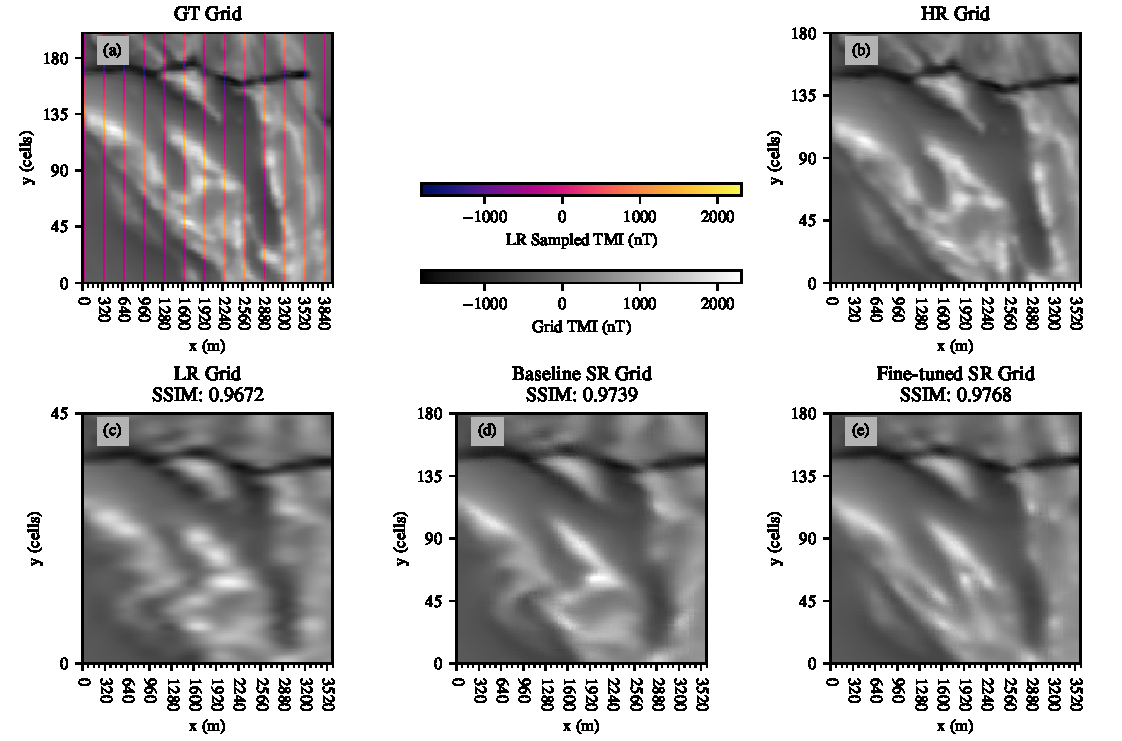
\includegraphics[width=1\linewidth]{fig/p2/srcomp_23.pdf}
        \caption[Super-resolution geophysics grid results I]{Super-resolution predictions on open access data, prepared using the proposed method.
            a) Ground truth, b) High-resolution, c) Low-resolution, d) Baseline super-resolution, e) Fine-tuned super-resolution.
        }
        \label{fig:srdata23}
    \end{figure}
\end{landscape}

\begin{landscape}
    \begin{figure}[hbtp]
        \centering
        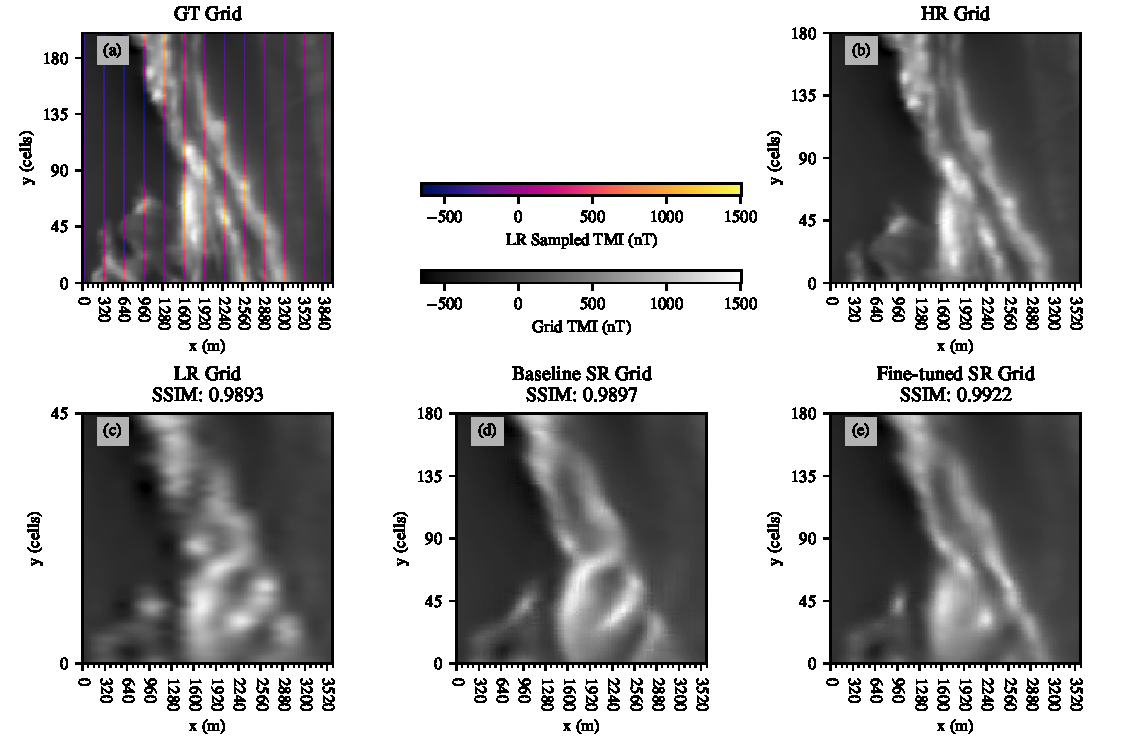
\includegraphics[width=1\linewidth]{fig/p2/srcomp_17.pdf}
        \caption[Super-resolution geophysics grid results II]{Super-resolution predictions on open access data, prepared using the proposed method.
            a) Ground truth, b) High-resolution, c) Low-resolution, d) Baseline super-resolution, e) Fine-tuned super-resolution.
        }
        \label{fig:srdata17}
    \end{figure}
\end{landscape}

\begin{landscape}
    \begin{figure}[hbtp]
        \centering
        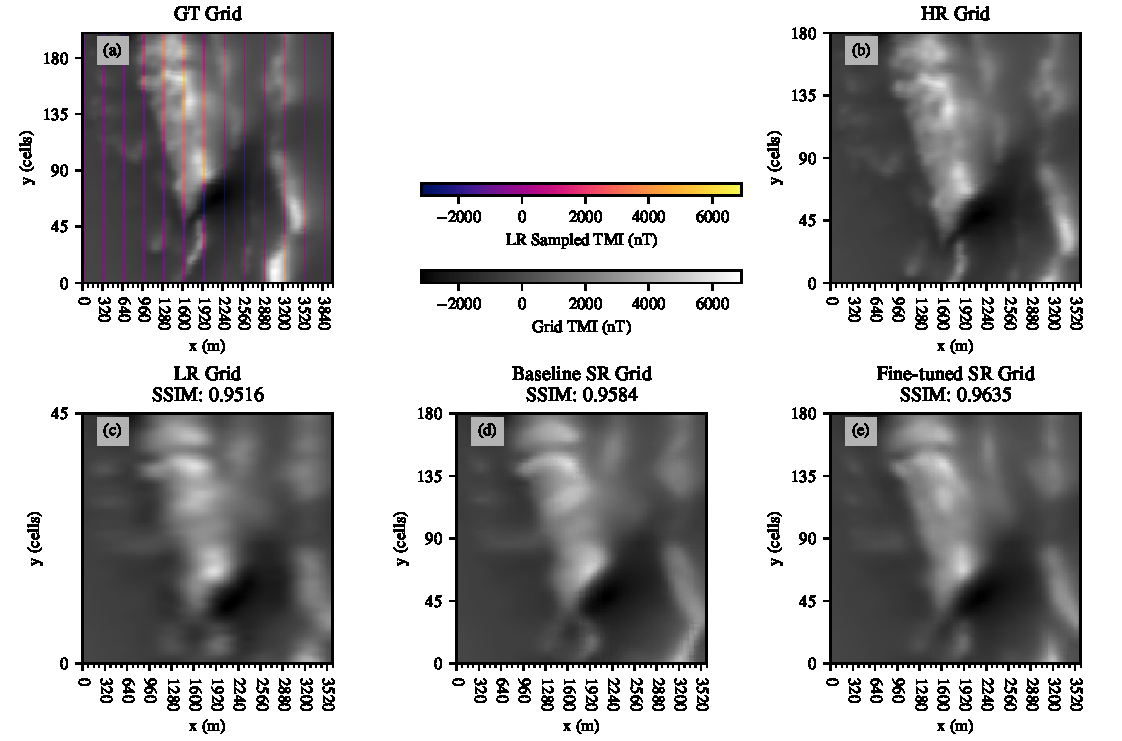
\includegraphics[width=1\linewidth]{fig/p2/srcomp_14.pdf}
        \caption[Super-resolution geophysics grid results III]{Super-resolution predictions on open access data, prepared using the proposed method.
            a) Ground truth, b) High-resolution, c) Low-resolution, d) Baseline super-resolution, e) Fine-tuned super-resolution.
        }
        \label{fig:srdata14}
    \end{figure}
\end{landscape}

\begin{landscape}
    \begin{figure}[hbtp]
        \centering
        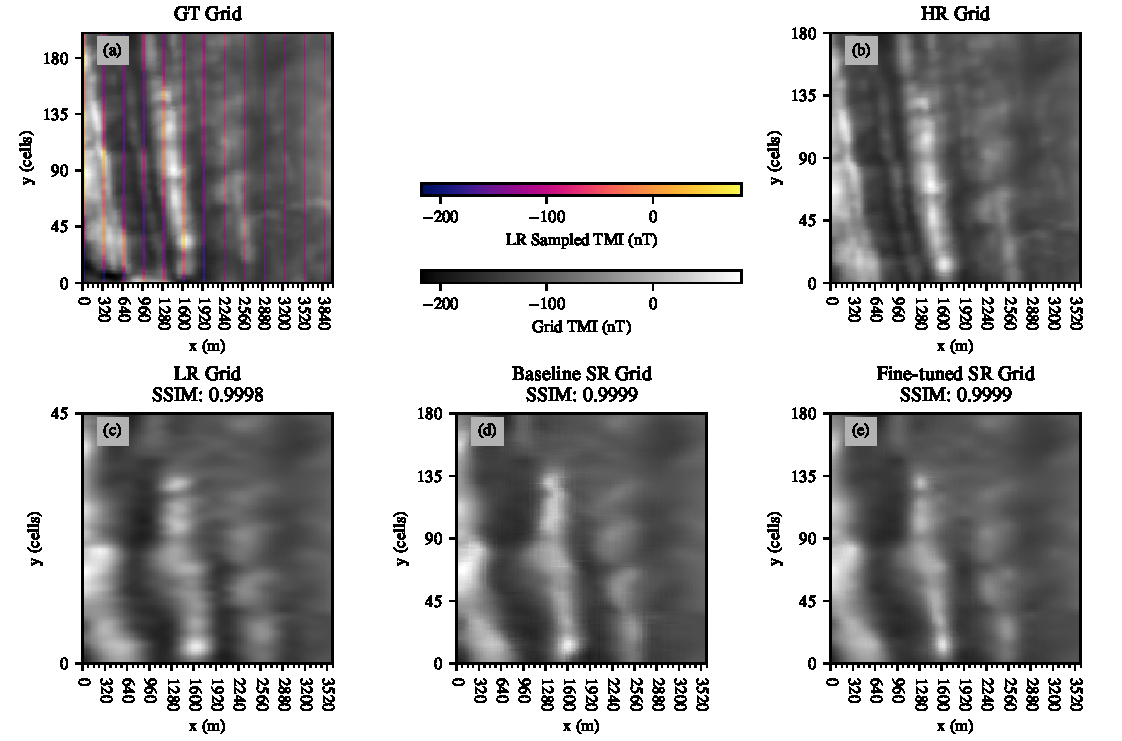
\includegraphics[width=1\linewidth]{fig/p2/srcomp_18.pdf}
        \caption[Super-resolution geophysics grid results IV]{Super-resolution predictions on open access data, prepared using the proposed method.
            a) Ground truth, b) High-resolution, c) Low-resolution, d) Baseline super-resolution, e) Fine-tuned super-resolution.
        }
        \label{fig:srdata18}
    \end{figure}
\end{landscape}


\section{Discussion}
\label{sec:2discussion}
The Noddyverse synthetic training dataset comprises geology models with a variety of realistic petrophysics and geological histories, and was sampled using simple but realistic airborne survey methodology.
Furthermore, real survey data used to fine tune the model were extracted from extents across a range of different terranes in Western Australia.
As such, the method and trained models generalise to the geological terranes represented in the Noddyverse and high-resolution state grid extents.
Granitic textures in real grid data are not represented in the synthetic Noddyverse training set, and show the least improvement by the method.
Different geological units present different features in magnetic potential field grids, with deformed igneous units typically causing abundant contextually important short-wavelength content.
These features, such as faulted or folded dykes, tend to show the most perceptual improvement in their structure following super-resolution upscaling.
This is due to the high performance of the method for reducing aliasing effects from the gridding process, and is apparent in the accurate reconstruction of linear features from discrete “string of beads” aliased features.
Long-wavelength features and smooth gradients, such as those present in sedimentary units or areas of cover are accurately upscaled in the proposed method, however these are also adequately upscaled with simple cubic spline interpolation of the low-resolution grid because they do not require predicted high frequency components.
The exception for super-resolution having higher quality is in areas of low magnitude TMI of only a few nanotesla across the entire extent.
In these cases, the otherwise minor noise introduced by the super-resolution process dominates the residual.

The synthetic forward models are associated with geological history class labels, providing an opportunity for more targeted fine-tuning by event history.
It is possible to filter the data to contain only the events of interest, which would prepare a baseline model targeting a single geological domain.
The baseline model prepared in this work demonstrated good performance across a range of geological domains, but may be improved for targeted domains using the filtered approach.

\section{Conclusion}
\label{sec:2conclusion}
An approach for upscaling geologically diverse geophysical survey grid data is proposed, which adopts transfer learning from synthetic data to better generalise super-resolution across different geological domains.
Using the preeminent LTE neural network architecture, synthetic magnetic forward models were used to prepare a baseline model capable of upscaling survey grids at four times scale.
Further, this baseline model was fine-tuned with open access survey grid data, prepared with a low-resolution transform appropriate for aeromagnetic geophysics.
Low-resolution features incorrectly enhanced by the synthetic baseline model were correctly resolved following fine-tune training with these data, and the model is capable of upscaling grids with \qty{320}{\m} line spacing to \qty{80}{\m} line spacing with an average FSIM score of \num{0.9731}.

% \section{Declaration of competing interest}
% The authors declare the following financial interests / personal relationships which may be considered as potential competing interests: This work was supported by a Rio Tinto Iron Ore PhD scholarship.

% \printbibliography{}


% \end{document}

\chapter{Implicit Neural Representation for Potential Field Geophysics}
\label{ch:paper3}
% \newrefsection{}
% % \documentclass[manuscript.tex]{subfiles}
% \documentclass[12pt,a4paper]{report} %,openright,twoside
% \usepackage{thesisstyle}
% \addbibresource{bib/PhD.bib}
% % \setcounter{chapter}{3}
% \begin{document}

\title{Implicit Neural Representation for Potential Field Geophysics}
\author[1*]{Luke Thomas Smith}
\author[1]{Tom Horrocks}
\author[2]{Naveed Akhtar}
\author[1]{Eun-Jung Holden}
\author[1]{Daniel Wedge}
\affil{Centre for Data-Driven Geoscience, School of Earth Sciences, The University of Western Australia (M006), 35 Stirling Highway, 6009 Perth, Australia}
\affil{Department of Computer Science and Software Engineering, The University of Western Australia (M002), 35 Stirling Highway, 6009 Perth, Australia}
\date{\today}
% \maketitle{}

\begin{abstract}
    The recent use of spatial coordinate features in multilayer perceptron (MLP) neural networks provides opportunities for novel applications in potential field geophysics.
    So-called coordinate MLP networks allow for learning a representative function of potential fields from their surveyed samples.
    % Using this new paradigm of encoding spatial information within a neural network enables new methods for working with potential field survey data.
    We present a novel method for implicit neural representation for potential fields, demonstrate the quality of the learnt implicit function by encoding real airborne geophysical survey line data, predict constant level grids, and compare the result to grid data processed with a traditional workflow.
    We further demonstrate the analytical calculation of gradients directly in the continuous domain using automatic differentiation, with the same framework used to train the neural network representation.
    Level grids queried from the learnt representation closely match the reference grid product, with a peak signal to noise ratio of 40 dB.
    Horizontal gradients calculated with this method are accurate against numerically derived gradients, while the vertical gradient is a poor match.
    The training process is rapid, and only requires recorded samples from a single survey extent.
\end{abstract}

\clearpage{}

\section{Introduction}
Geophysical potential fields are routinely collected and used to assist the understanding of the subsurface for geoscience and mineral exploration.
When surveying these fields, which are continuous functions in three dimensions, sample locations are scattered in \(x\), \(y\), and \(z\), despite best efforts to conform to a regularly spaced line or grid acquisition plan.
These scattered data are typically regularised to a quantised grid for subsequent interpretation, which imposes a new limit on high frequency content and gives rise to spurious artefacts that are a product of the gridding process, not the surveyed field.
% The interpolation process may 

Neural networks can be considered as universal function approximators.
The recent technique of deep learning implicit neural representation (INR) \parencite{mildenhallNeRFRepresentingScenes2020} represents a signal as a function of its coordinates, built on a network architecture known as a coordinate multilayer perceptron (CMLP) (see \textcite{ramasinghePeriodicityUnifyingFramework2022} for a recent introduction).
By parameterising the function in coordinate space, novel values of the function can be queried at arbitrary coordinates within the learnt continuous spatial domain.
Recent advances in CMLPs by using periodic activations such as sinusoids have demonstrated that high frequency information can be modelled well by CMLP networks, while being continuously differentiable throughout the depth of the network.

We present a novel method of encoding a representation of a geophysical potential field using INR\@.
This method contributes a novel method of creating level grids from scattered aeromagnetic data.
In our method, due to using a continuous coordinate representation, there is no dependency on grid quantisation from an initial cell size selection.
The proposed technique also provides for further processing that can be calculated analytically in the continuous spatial domain, allowing the use of all available sample information in these calculations.

%TODO - a bit abrupt
For the task of level grid prediction, the PSNR similarity between a case study reference grid and the proposed method is \qty{39.97}{\dB}.
Additionally, directional derivatives of the implicit representation calculated numerically and using automatic differentiation are shown, with mean residuals of \qty{0.4} and \qty{0.8}{\nano\tesla\per\m} for the easting and northing derivatives respectively, albeit vertical derivative performance remains limited.

INR and CMLP have recently emerged in the literature, and our proposed method stands to benefit from ongoing research in these highly active fields.

\subsection{Geophysical sampling and regularisation}
\label{sec:geo_airborne}
Airborne or ground-based potential field surveys sample a magnetic (or gravitational) scalar field on a three-dimensional drape surface.
Cultural obstructions or topography within the survey extent cause this drape surface to be irregular, and the sample points scattered.
The resolvable detail within the sampled field is a function of the sampling density, and the distance from the source.
To enable digital processing of the sample data following acquisition, the scattered points are regularised to a quantised grid.
The Nyquist wavelength inherent to the selected grid cell size during regularisation limits the high-resolution information representable by the grid.
Because this regularisation is one of the earliest steps in preparing data for subsequent interpretation and processing tasks, the information lost cannot be used in these later tasks.
% Subsequent processes such as frequency filtering or directional gradients are similary constrained by the parameters of the regularisation.
% Additionally, storing the grid product requires amount of memory, to represent the value with adequate precision at each cell in the resulting grid.

% \label{sec:geo_physics}
Magnetic and gravitational fields in geophysics are conservative vector fields but are typically sampled as a scalar potential field in a single direction.
Representing a vector field requires three orthogonal components at each spatial coordinate, while a scalar field can be parameterised with a single component \parencite{blakelyPotentialTheoryGravity1996}.
A potential field survey can be parameterised as
\begin{equation}
    \label{eqn:potential}
    \phi\left(x,y,z\right),
\end{equation}
where \(\phi{}\) is the potential, and \({(x,y,z)}\) are the three spatial dimensions.

\subsection{Implicit neural representation}
\label{sec:inr}
Coordinate Multilayer Perceptron (CMLP) networks are fully connected networks, which have been ubiquitous in machine learning for several decades.
An MLP comprises a sequence of layers of neurons, densely connected to all neurons in each adjacent layer.
Each neuron is a discrete trainable function, comprising a weight multiplied by the input vector, an added bias term, and a subsequent scaling function termed the activation function.
The structure of an MLP can be described by the number of neurons in each layer (features), the number of layers between the input and output (hidden layers), and the class of activation function used.

A classic example of an MLP is using an input vector of image pixel intensities \(u\), and an output vector of class labels \(l\).
Training this example network with a large number of different images with class labels produces a model capable of predicting the class of novel input image vectors.
A CMLP for representing images instead takes an input of explicitly stated pixel coordinates \((x,y)\), and an output vector of image pixel intensities \(u\) at those coordinates.
Thus training of a CMLP network requires a set of input coordinates and intensities from a single image, and results in a model capable of predicting the intensity of any arbitrary continuous coordinate within the input domain.
Both tasks may use similar images and an MLP network structure with the same \(n\) hidden layers and \(m\) features, but the use of coordinates as inputs and intensities as outputs changes the predictive task.
CMLP networks for predicting 3D scalar fields are a class of neural networks \(f\) which train \(u = f(x,y,z)\), with \(u\in\mathbb{R}^1\) and \((x,y,z)\in\mathbb{R}^3\).

Seminal work by \textcite{mildenhallNeRFRepresentingScenes2020} demonstrated INR of volume density and colour radiance, learnt from five dimensions of spatial coordinates and orientation.
Their approach uses positional encoding to improve the learning capacity of high-frequency content, addressing the issue of spectral bias in deep learning \parencite{rahamanSpectralBiasNeural2019}.
When replacing positional encoding and the ReLU activation with periodic activation functions such as the sinusoid \parencite{sitzmann2019siren} the high frequency representation of CMLP networks is significantly enhanced.
Periodic activation functions differ from typical non-linear activations by comprising the neuron with a function that repeats periodically, which allows for continuous differentiation throughout the depth of the network.
Work by \textcite{ramasinghePeriodicityUnifyingFramework2022} revealed that it is the magnitude of the first and second derivatives of the activation that enhanced high-frequency representation learning capacity, rather than periodicity, leading to Gaussian \parencite{ramasinghePeriodicityUnifyingFramework2022} and wavelet \parencite{saragadamWIREWaveletImplicit2023} activation functions for CMLP\@.

CMLPs can be used for a variety of computer vision tasks, including three-dimensional point cloud representation \parencite{qiPointNetDeepHierarchical2017}, and two-dimensional natural image representation tasks such as super-resolution and infilling \parencite{leeLocalTextureEstimator2022, chenLearningContinuousImage2021}.
Resolution in these tasks is not limited by quantisation of the representation, but rather the capacity of the network architecture used.
Increasing this capacity is currently the subject of high interest in the machine learning research community.
Research directions include leveraging new activation functions \parencite{saragadamWIREWaveletImplicit2023}, transforming the input space \parencite[e.g.][]{benbarkaSeeingImplicitNeural2022} or using additional constraints on the search space such as physics-informed neural networks \parencite{raissiPhysicsinformedNeuralNetworks2019}.
In geoscience, INR has been used for numerical modelling \parencite{hillierGeoINRImplicitNeural2023}.

CMLP networks for INR can be compared to compressed sensing \parencite{candesIntroductionCompressiveSampling2008} for their ability to recover accurate grids from sparsely sampled geophysics samples.
While recovery of potential field grids using a compressed sensing approach is often framed as a numerical optimisation problems \parencite[e.g.][]{yangAirborneGravimetryData2015,xuGravityAnomalyReconstruction2019}, these are not equivalent to modern deep learning approaches.
Compressed sensing relies on the theory that a signal has a sparse representation in some transform domain, and a deeper exploration of the comparison between INR and compressed sensing remains to be performed.
Compressed sensing recovers the signal through linear transformations, while neural networks allow convenient modelling of non-linear transformations.

\subsection{Automatic Differentiation}
Automatic differentiation (AD) refers to one of several methods for computing derivatives, specifically to the method of accumulating derivatives during function evaluation \parencite{baydinAutomaticDifferentiationMachine2018}.
This method underpins modern machine learning frameworks such as Pytorch \parencite{paszkePyTorchImperativeStyle2019}, which is used to construct the network architecture and perform training in this work.
In these frameworks, training is performed by evaluating a set of inputs using the current model parameters during a forward pass, while accumulating the partial derivatives of the result with respect to those parameters, to optimise an objective (loss) function.
These gradients inform parameter update operations to minimise the model loss.
However, automatic differentiation can also evaluate the derivatives of the network output with respect to the inputs, using the same high-performance AD framework.
This can directly provide the partial derivatives of the potential field with respect to its coordinates \(\frac{\partial\phi{}}{\partial x}, \frac{\partial \phi{}}{\partial y}, \frac{\partial \phi{}}{\partial z}\), as well as higher order derivatives, without first requiring gridding.

% Per naveed - > start of sec 1.3?
\subsection{Overview of the proposed method}
\label{sec:overview}
The proposed method leverages recent approaches in the literature to learn a continuous three-dimensional representation of potential field geophysics extents, using INR\@.
This implicit representation is used to generate two-dimensional levelled grids directly from scattered sample data, by querying the representation with regularly spaced grid nodes at a constant level.
Partial derivatives can be calculated on the representation itself, remaining in the continuous coordinate domain.
These are compared against a case study reference grid from Geoscience Australia, with gradients from numerical derivative calculation.
% An overview diagram is presented in \Cref{fig:overview}.

% \begin{figure}[hbtp]
%     \centering{}
%     % \includegraphics[width=0.5\linewidth]{fig/p3/overview.pdf}
%     \caption[Overview of the proposed method]{Overview}
%     \label{fig:overview}
% \end{figure}

\section{Method}
\subsection{Data}
The case study is performed using data from the 2002 Wolfe Creek meteorite impact magnetic survey \parencite{wolfecreek2019}.
This high-resolution survey contains \qty{402} line-kilometres of data at \qty{50}{\m} line spacing with a nominal terrain clearance of \qty{40}{\m}, with line data collected on North-South transects.
Prominently featured in the survey are the circular crater rim, and two East-West trending linear dune features to the North of the survey extent.
The data used for implicit representation excludes the survey tie lines, typically used in airborne geophysical surveys to reduce inter-line levelling noise.
The mean altitude of the drape surface excluding tie lines is \qty{39.5}{\m}, with a standard deviation of \qty{4.5}{\m}.
The sample locations and recorded altitudes are shown in \Cref{fig:samples}, where it can be seen the crater rim topography causes large deviations in elevation from the nominal drape.

\begin{figure}[hbtp]
    \centering{}
    \includegraphics[width=\linewidth]{fig/p3/P864_sample_locs.pdf}
    \caption[Point samples]{Sample altitudes for the Wolfe Creek survey lines. The diverging colourmap has been centred at the nominal survey terrain clearance of \qty{40}{\m}.}
    \label{fig:samples}
\end{figure}

Both the line data and grid raster netCDFs for the Wolfe Creek survey were downloaded from Geoscience Australia \footnote{https://pid.geoscience.gov.au/dataset/ga/142694} (GA) and used without further processing.
The line data netCDF contains tie-levelled, micro-levelled, and AWAGS levelled magnetic variables, in increasing stages of processing respectively.
The micro-levelled magnetic data are used in this case study because the original sample altitude is uncertain in the available levelled data.
Either a geographic and projected coordinate system can be used, provided the query coordinates for inference match those used during training.
The three spatial coordinate dimensions are independently and linearly min-max normalised between \num{-1} and \num{1}.
While this means the axes in the latent spatial domain may be compressed relative to each other axis, the inverse normalisation process returns proportionality between axes.
The case study data do not span a large or magnetically varying geological extent, hence it is sufficient to use simple min-max normalisation for the magnetic field data within the global extent of the survey samples, here between \num{-1} and \num{1}.
If extensive or complexly varying magnetic provinces were present within the dataset, a normalisation method more robust to outliers may be required.
The \num{76420} sample points contained within the case study line data are split, with \qty{70}{\percent} used for training, and a random \qty{20}{\percent} of the remaining points are reserved to validate the model performance during training.
Inference is performed by querying novel coordinates within the learnt domain, here at regularly spaced grid intervals for comparison with standard grid regularisation methods.

\subsection{Network architecture}
The CMLP architecture comprises a simple fully connected network with \(n\) hidden layers, each with \(m\) neurons. %, presented within \Cref{fig:overview}.
The number of input features is 3, for each spatial dimension, and the number of output features is 1, for the predicted potential field value at those coordinates.
Comparison of recently proposed activatons and hyperparameters for CMLP is performed by \textcite{saragadamWIREWaveletImplicit2023}, where increasing both \(n\) and \(m\) increases the capacity of the model, at the cost of computational requirements.
High quality implicit representation is typically achievable with the number hidden layers between \num{3} and \num{8}, and number of neurons per layer up to \num{256}.
Empirically, the quality of the high-resolution representation continued to improve with increasing both \(n\) and \(m\).
Therefore, the presented method uses \num{8} hidden layers and \num{256} neurons per layer, which achieves good quality results in rapid time and within the system memory constraints.
The sinusoidal activation of \textcite{sitzmann2019siren} is used.
The WIRE or Gaussian activations were empirically less robust to hyperparameter selection, and did not return high-quality representation for the magnetic geophysics grids.

\subsection{Training setup}
\label{sec:training}

Implicit functions are trained using coordinate-value pairs.
For low-resolution inputs the entire cell coordinate and cell value dataset fits within GPU memory for batch gradient descent.
The Wolfe Creek meteorite impact crater case study line data has \num{76420} sample points, and the Geoscience Australia provided reference grid has a resolution of \numproduct{446 x 445} cells.
The entire case study line data fit in a single batch within the available graphics memory, and can be trained using batch gradient descent.
Each sample in the batch is a single 3D survey point with the associated 1D target potential field value.
% However, if training on larger aeromagnetic surveys, memory becomes a constraint and mini-batch training is required.

Training was performed on an Intel i9-10900KF workstation with an Nvidia RTX 3090 24 GB GPU\@.
A highly accurate representation can be learned within \qty{5000}{epochs} using the Adam optimiser, for a duration in the order of \qty{60}{seconds}.
The objective function comprises \(L^2\) loss between the input and predicted field values \(u\),

\begin{equation}
    \label{eqn:cri}
    \mathcal{L}_{Total} = \lVert{}u_{input} - u_{pred}\rVert{}_{2}. % + \beta{} \lVert{}\frac{\partial^{2}{u_{pred}}}{\partial{}\phi{}_{pred}^{2}}\rVert{}_{2}
\end{equation}

The OneCycle learning rate scheduler \parencite{smithSuperconvergenceVeryFast2018} with a maximum rate of \num{1e-4} is used to provide fine tuning at low learning rates toward the end of training.
The very low learning rates in the late stages of training significantly contribute to the quality of the representation when compared to a constant learning rate.
Convergence of the network is shown in \Cref{fig:convergence}.


\begin{figure}[hbtp]
    \centering
    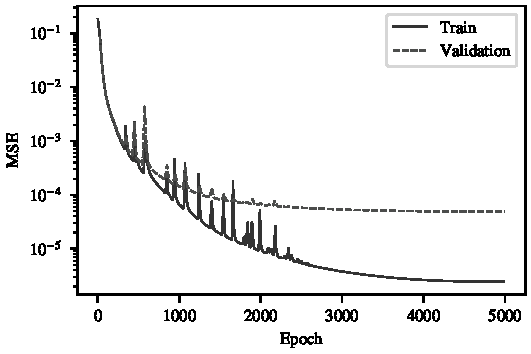
\includegraphics[width=0.5\linewidth]{fig/p3/loss_plot.pdf}
    \caption[Training convergence]{Train and validation loss for the duration of the experiment.}
    \label{fig:convergence}
\end{figure}

\subsection{Derivative calculation}
A naive approach to calculating gradients with the trained INR would be to evaluate the representation \(f(x, y, z)\) at a set of coordinates \({(x, y, z)}_1 \dots {(x,y,z)}_n\), and use numerical differentiation with the output grid to calculate derivatives.
However, using AD with Pytorch, the implicit representation can be differentiated with respect to its coordinate inputs to provide spatial gradients, prior to being queried at the nodes of a quantised grid.
That is, to directly sample \(\nabla{}\phi{}_{(x,y,z)}\) at \({(x, y, z)}_1 \dots {(x,y,z)}_n\).
Higher order derivatives can be calculated using AD in the same manner, but are not presented here.

\section{Results}
\subsection{Level grid prediction from INR}
Querying a learnt INR using a regularly spaced \(x,y\) grid at a specific \(z\) height is a novel method for producing level grids from geophysical potential field surveys.
The cell size can be selected using a finer or coarser \(x,y\) spacing, including variable or anisotropic cell sizes.
Contemporary super-resolution research can leverage this continual representation as a framework for high quality arbitrary scale factor high-frequency signal prediction \parencite[e.g][]{chenLearningContinuousImage2021}.
However, the potential field representation task here does not attempt to predict additional high-frequency information and resolution remains determined by the neural network's capacity to represent high frequencies sampled by the survey line spacing.

\Cref{fig:grid40} shows the INR queried at \(z=\qty{40}{\m}\), which is the nominal terrain clearance of the survey.
A good qualitative match is achieved between the GA reference grid and the grid queried from the implicit representation, which successfully reconstructs the linear dune features and circular rim features.
This high performance is quantified by the residuals and peak signal to noise ratio (PSNR) of \qty{40.12}{\dB}, with mean residuals of \qty{0.4} and \qty{0.8}{\nano\tesla\per\m}
% Further level grids from other survey extents are included in Appendix A.

\begin{figure}[hbtp]
    \centering
    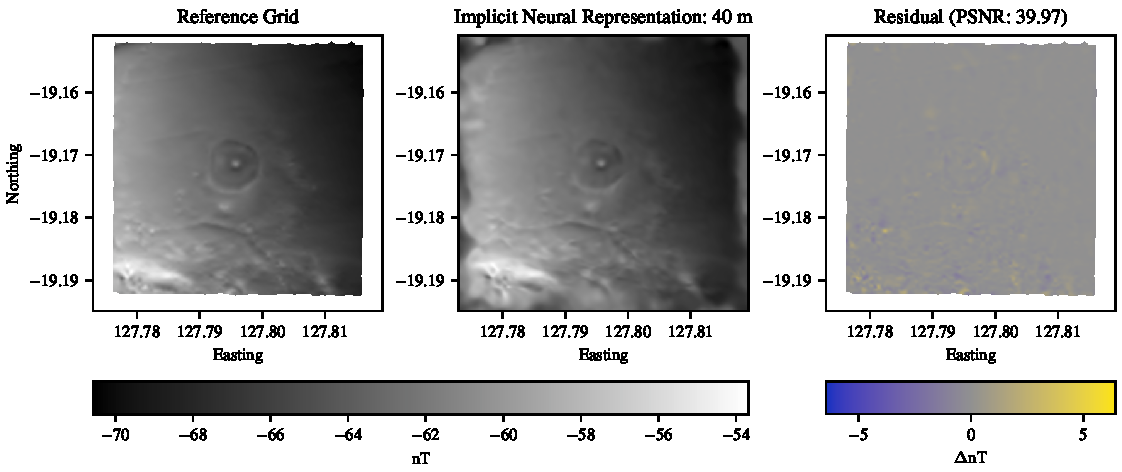
\includegraphics[width=1.0\linewidth]{fig/p3/P864_grid_comparison_40m.pdf}
    \caption[Grid prediction at the nominal altitude]{Comparison between the reference grid processed by Geoscience Australia (left) and the constant level grid queried from the INR at \qty{40}{\m} (middle). The residuals are shown for areas containing reference data (right), with a range of ±2 standard deviations of values in the reference grid.}
    \label{fig:grid40}
\end{figure}

The INR can be queried at arbitrary continuous coordinates, including out-of-range values beyond the training domain.
As expected, the predicted field becomes unrealistic when extrapolating beyond this boundary, which can be seen in the periphery of the INR grid in \Cref{fig:grid40}.
This boundary region (indicated by solid white in the reference grid) is excluded from PSNR calculation.

Constant level grids can be queried from the INR at any height.
\Cref{fig:grid35} shows the case study INR queried at \qty{35}{\m}, which is \qty{5}{\m} lower than the nominal survey altitude.
While the rim feature can still be interpreted within this lower level grid, the INR fails to demonstrate physically realistic continuation of the field.
% It is conjectured that successfully training a PINN criterion such as Laplace’s equation loss (equation 1.3) would improve the accuracy of these upward or downward extracted slices. 

\begin{figure}[hbtp]
    \centering
    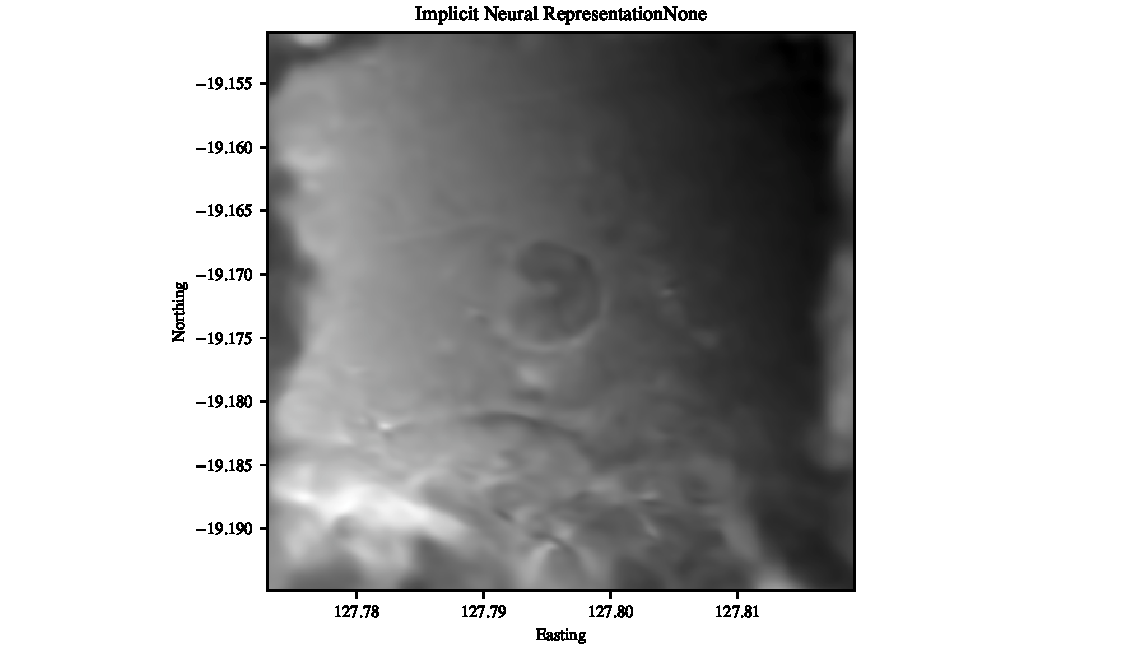
\includegraphics[width=1.0\linewidth]{fig/p3/35_level_grid.pdf}
    \caption[Grid prediction outside the nominal altitude]{A constant level grid queried from the INR at the height of \qty{35}{\m}.}
    % AWAGS is 80 m, but we see nothing useful at 80m
    \label{fig:grid35}
\end{figure}

% The strong performance of the model is retained even when using a subsampled training dataset, here shown at \qty{30}{\percent} and \qty{10}{\percent} (\Cref{fig:gridpct}) of the total available data.
% % In both cases, the validaiton and test sets remain identical to the initial training split.

% \begin{figure}[hbtp]
%     % \includegraphics[]{fig/p3/grid_subpct.pdf}
%     \caption[Grid subsampled]{Performance of level grid prediction shown at \qty{30}{\percent} and \qty{10}{\percent} random sampling of training data.}
%     \label{fig:gridpct}
% \end{figure}


\subsection{Spatial derivatives}
Using AD, derivatives can be calculated between the input spatial coordinates and the output potential field representation.
For comparison, the derivatives calculated with AD are compared with numerical derivatives calculated on the level grid queried from the same INR model.
While horizontal derivatives queried from the INR correspond well to numerical derivatives calculated on the \qty{40}{\m} level grid in \Cref{fig:horigrad}, the vertical derivative shown in \Cref{fig:vertgrad} suffers poor performance.
This correlates with the poor continuation performance of model when predicting level grids several metres or more beyond the nominal sample height.
This is interpreted as the presented model having a limited capacity to extrapolate beyond the flown data extent, and learning a poor representation of the vertical component of the potential field, which we further discuss in \Cref{sec:3discussion}.
\begin{figure}[hbtp]
    \centering{}
    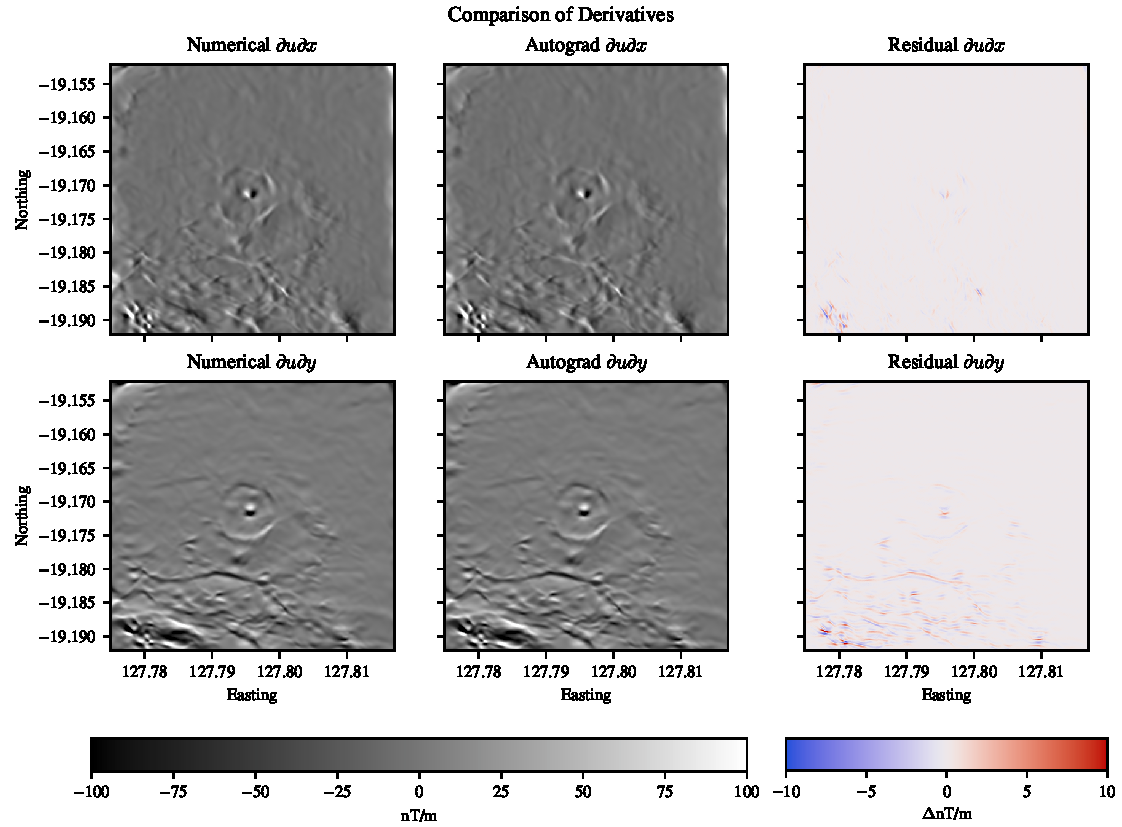
\includegraphics[width=1.0\linewidth]{fig/p3/P864_dh_comparison.pdf}
    \caption[Horizontal derivatives]{Horizontal gradients calculated using the proposed method and the reference numerical method.
        Both numerical differentiation (left column) and AD INR (middle column) are calculated on the INR level grid or INR respectively.
        Residuals are calculated between the numerical and AD gradient grids (right column).}
    \label{fig:horigrad}
\end{figure}

\begin{figure}[hbtp]
    \centering{}
    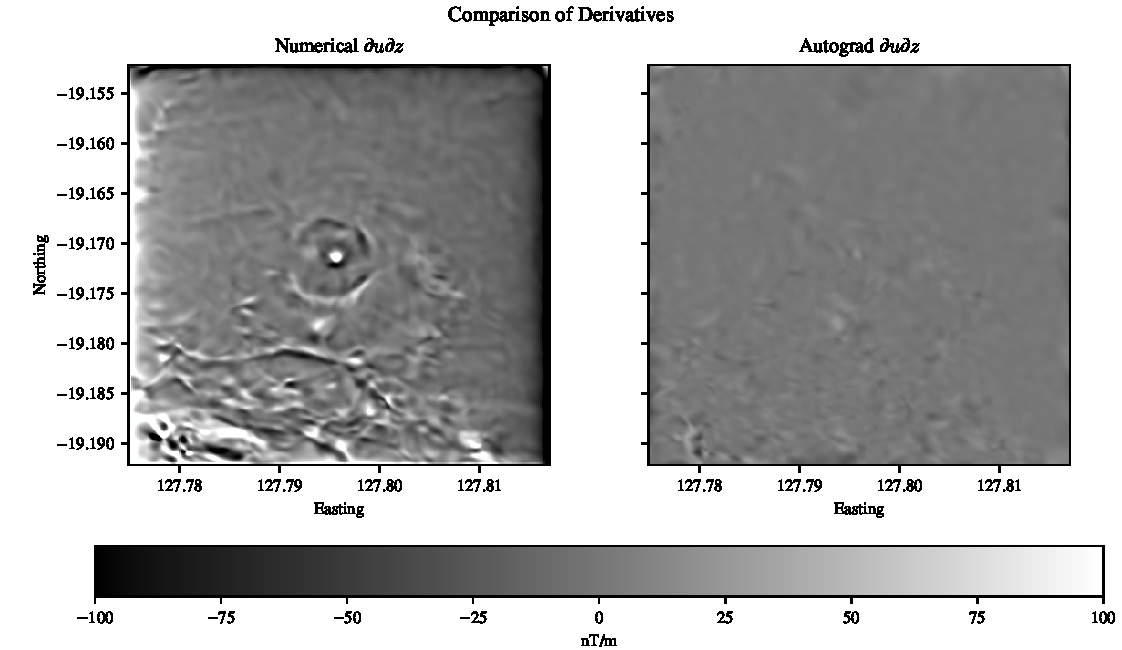
\includegraphics[width=1.0\linewidth]{fig/p3/P864_dv_comparison.pdf}
    \caption[Vertical derivative]{Vertical derivative grids queried from AD differentiated INR (left) and calculated numerically (right) on the \qty{40}{\m} level grid queried from the INR\@.
     The proposed method has poor vertical gradient representation, possibly due to the single height sampled in aeromagnetic survey design.}
    \label{fig:vertgrad}
\end{figure}

\section{Discussion}
\label{sec:3discussion}
The proposed method has strong learning capacity for the potential field samples in the horizontal plane near the nominal survey altitude, allowing extraction of level grids which are accurate against the reference grid.
Level grids can be queried at arbitrary heights and cell sizes, with the highest accuracy achieved at the realised nominal survey altitude.
Performance decreases within approximately one standard deviation from that height (\qty{35} to \qty{45}{\m}), with gradual failure of the model outside of that range.
It is interpreted from the poor quality of the vertical gradients and out-of-range level grid predictions that the model is learning a function between horizontally coplanar points, and not an accurate vertical continuation function.
This is conjectured to be caused by aeromagnetic sampling being carried out on a nominally horizontal planar drape surface, without sufficient repeat measurements at other heights to train the network for the vertical field component.

While quantised grids can be queried at any cell size, short wavelength information beyond the Nyquist limit of the survey line sampling are not predicted with this architecture.

The current method could include additional target dimensions, which would allow representation learning of vector fields \(\mathbb{R}^{3}\) in three dimensions \(\mathbb{R}^{3}\).
This has applications in tensor fields and data integration tasks, and these remain for future work.

INR is a rapidly evolving field of research, and draws on contemporary established deep learning improvements within related fields.
In addition to improving the high-frequency learning capacity with novel activation functions and regularisation methods, fundamental neural network research and hardware development is ongoing.

% Even when using a small subset of the dataset, this performance is retained.

% The case study survey presented is very small compared to typical regional aeromagnetic surveys.
% A demonstration of the method on a large aeromagnetic survey, requiring minibatch training, is included in \Cref{app:menzies}.
% Training of this representation follows the parameters outlined in \Cref{sec:training}, which were optimised for the Wolfe Creek case study, with the addition of a shuffled minibatch size of \qty{1024000}\@.
% Attempts to train the CMLP with small batch sizes did not converge.%, reflecting the non-convergence result found for training on very large subsampling factors of the line dataset.


\subsection{Future Work}
\label{sec:future}
The outputs of neural networks can be constrained to obey geophysical laws, using physics-informed neural networks (PINNs) \parencite{raissiPhysicsinformedNeuralNetworks2019}.
PINNs recognise that if the inputs to a neural network are samples of a function which follows some physical law, outputs from the model should similarly be constrained by that law.
By regularising the network with an objective function which penalises solutions that don't fit the partial differential equations describing the law, it is possible to vastly reduce the physically valid solution search space \parencite{raissiPhysicsinformedNeuralNetworks2019}.
Because CMLP networks with periodic activations are continuously differentiable, it is possible to enforce this constraint as an element of the overall loss function within the network.
\Textcite{sethiHardEnforcementPhysicsinformed2023} demonstrate that this regularisation does not have to be implemented as a loss function, but instead can be a hard constraint embedded within the network.
Another approach \parencite{liImplicitStochasticGradient2023} replaces the ubiquitous stochastic gradient descent optimiser \emph{Adam} with an implicit stochastic gradient descent (ISGD) method.

Examples of physics-informed constraints include enforcing initial or boundary conditions, or conforming to known properties of the modelled signal.
Potential fields in an airborne sampling context are constrained by a number of physical laws, including \emph{Laplace's equation};
\[
    \nabla^2 \phi = 0,
\]
or denoted in three dimensions,
\begin{equation}
    \label{eqn:Laplace}
    \frac{\partial{}^2\phi}{\partial{}x^2} + \frac{\partial{}^2\phi}{\partial{}y^2} + \frac{\partial{}^2\phi}{\partial{}z^2} = 0.
\end{equation}

Inspired by the approach of \textcite{raissiPhysicsinformedNeuralNetworks2019}, a geophysics-informed network could include a Laplace criterion,
\begin{equation}
    \label{eqn:crilaplace}
    \mathcal{L}_{PDE} = \frac{1}{S_i}\sum_{i=1}^{S_i} \left(\frac{\partial{}^2f}{\partial{}x^2} + \frac{\partial{}^2f}{\partial{}y^2} + \frac{\partial{}^2f}{\partial{}z^2}\right)^2,
\end{equation}
where \(S_i\) indicates the \(i^{th}\) sample point of the field survey \(\phi(x, y, z)\).
This criterion penalises outputs where Laplace's equation is not satisfied because the sum of partial second derivatives is not close to zero.

%     \mathcal{L}_{PDE} = \lVert{}\frac{\partial{}^2f}{\partial{}x^2} + \frac{\partial{}^2f}{\partial{}y^2} + \frac{\partial{}^2f}{\partial{}z^2}\rVert{}_{2}
%TODO Confirm logic here: % If Laplace's equation:\( \nabla^2 \phi = 0 \) is satisfied, it is harmonic, and has continuous single valued first derivatives, and has second derivatives.
% This indicates the function lacks curvature. 
% Blakely:
% A force field \(F\) is the gradient (or negative gradient) of the potential energy.
% \( F = \nabla\phi \) for the gravity potential, \(F = - \nabla \phi\) for the Magnetic potential.
% \( \phi(x,y,z) = constant \) is an equipotential surface.
% Numerical methods for potential field continuation are unstable, recognised in the geophysical community by solution divergence and noise in predictions.

Initial attempts using the objective function approach were trialled in this work, but struggled to converge and remain for future work.
It may be worth investigating other geophysical formulae for PINN implementation, such as vertical continuation described in \textcite{blakelyPotentialTheoryGravity1996}.

\section{Conclusions}
High-resolution implicit neural representation of potential field geophysics surveys is achieved with the use of coordinate MLP neural networks for INR\@.
Resolution in the representation is limited by network capacity, rather than initial grid cell size selection during regularisation.
Level grids can be extracted from these representations, emerging as a novel method for regularising scattered geophysical sample data.
Sptaial gradients can be calculated directly from the learnt representation, and can be queried at arbitrary locations.
Regularly sampled grids of the gradients are near-identical to those calculated by existing numerical methods, and benefit from being gridded after gradient calculation.

\section{Acknowledgements}
This project is funded by a Rio Tinto Iron Ore PhD scholarship.

\printbibliography{}

% \section{Appendix A}
% \label{app:menzies} %TODO format as "Appendix"
% The Menzies North P864 survey contains xxx sample points across yyyy line kilometres, and was flown at a nominal terrain clearance of zz m.
% While a high-quality result is attainable using batch gradient descent on a subset of the survey points, minibatch gradient descent is demonstrated for the CMLP used to learn the full survey INR\@.


% \begin{figure}[hbtp]
%     % \includegraphics[width=\textwidth]{fig/p3/menzies.pdf}    
%     \caption[Menzies INR]{Level grid representation using minibatch gradient descent.}
%     \label{fig:vertgrad}
% \end{figure}


% \end{document}

% \newrefsection{}
% % \documentclass[manuscript.tex]{subfiles}
% \documentclass[12pt,a4paper]{report} %,openright,twoside
% \usepackage{thesisstyle}
% \addbibresource{bib/PhD.bib}
% \setcounter{chapter}{4}
% \begin{document}

%brings together the key findings and contributions of the research as a whole
% provide a synthesis of the work as a whole presented in the body of the thesis.
% It is important that this final chapter demonstrates the collective contribution to knowledge provided by the research described in the thesis,
% and provide overall conclusions that address the research aims.

\chapter{Future work}
\label{ch:futurework}
The outputs of machine learning models are regarded with apprehension in geophysics practice due to the perceived “black box” of these methods \parencite{delaatAlgorithmicDecisionMakingBased2018,rudinStopExplainingBlack2019}, and the impact these models may have on subsequent interpretation.
As widely accepted by the geoscience community, all models are wrong, but some models are useful, and this extends to machine learning models.

When a domain expert encounters low-resolution grid data, they may observe which gridding method was used, the line spacing and direction, and form their understanding of potential aliasing and spurious anomalies in the grid accordingly.
Assisted by this understanding, they can infer geological features with varying degrees of confidence.
The SR method however does not consider these constraints, because imputation is purely based on features extractable by the model.
This was demonstrated to introduce noise or artefacts during SR inference, as well as the incorrect enhancement of artefacts in low-resolution data such as aliased geological strike.
However, given the uncertainty of geological interpretation of geophysics data \parencite{sivarajahIdentifyingEffectiveInterpretation2013} SR outputs may be used as an auxiliary data when interpreting low-resolution magnetic features.
The domain expert can then use the SR grid to reassure or reassess the original low-resolution grid interpretation and improve their confidence accordingly.

Super-resolution for geophysics is not yet characterised and requires further efforts towards improving reliability before wide-spread adoption in practice.
This section proposes four avenues for future research:
\begin{enumerate}
    \item{} Exploring the impact on geological mapping from the use of SR,
    \item{} Understanding the impact of choices in training super-resolution for domain specific tasks,
    \item{} Identifying an improved image quality assessment for gridded potential field data and,
    \item{} Investigating the use of a physics-informed approach for SR and implicit representation.
\end{enumerate}

\section[Super-resolution impact on geological interpretation]{The impact of super-resolution on geological interpretation}
The super-resolution outputs from the methods presented in this thesis have improved structural accuracy over the low-resolution grids.
This is likely to have a positive impact on the detection of features such as lineaments and unit boundaries for geological interpretation from magnetic data.
However, despite the reduction of introduced structural inaccuracies with the use of open access training data in \Cref{ch:paper2}, it is likely that some features with specific structural geometries will still be incorrectly super-resolved.
A domain expert may be able to recognise structures that are inconsistent using auxiliary information and the regional geological context, but machine processed super-resolution grids will use these data as provided.
In order to improve the adoption of SR for geological interpretation from potential field data, a rigorous study of the impact of SR on interpretation outcomes is required.
This could be a geological mapping task, such as the reinterpretation of regional geology using super-resolution upscaled regional magnetic TMI grids.
Comparison could then be made for the accuracy and benefit of a super-resolution method compared to the existing low-resolution interpretation.
However, such analysis will be difficult to perform with respect to different interpreters' variability in pattern recognition, especially in the context of their confidence in the reliability of the super-resolution product.
Previously, \textcite{sivarajahIdentifyingEffectiveInterpretation2013} reported significant variability between individuals when detecting geological targets from magnetic geophysics data.
A more reliable, repeatable and quantifiable approach would use automated pattern recognition methods developed for geophysical features.
For example, the automated lineament detection technique of \textcite{holdenAutomaticIdentificationResponses2011,holdenAutomatedAnalysisRegional2008} could be applied to low-resolution and SR grids, to compare their delineated features.

\section[Super-resolution for domain specific tasks]{A structured approach to training super-resolution for domain specific tasks}
Several models were implemented throughout \Cref{ch:paper1,ch:paper2}, namely RDN\textdaggerdbl{}, ESRGAN+, and LTE\@.
% However, the most important choice in developing a performant super-resolution neural network for real-world aeromagnetic survey data was the choice of training data.
The work in \Cref{ch:paper1} was prepared for publication prior the release of a large and varied synthetic geology training dataset \parencite{jessellNoddyverseMassiveData2022}.
It was seen in \Cref{ch:paper2} that this data improved model performance for a range of features by using transfer learning for pre-training.
% This transfer learning approach for training data is also found to be useful for RDN\textdaggerdbl{} and ESRGAN\@.
Here, the use of synthetic and real-world line spacing sampled data approach used with LTE in \Cref{ch:paper2} are adopted for the RDN\textdaggerdbl{} and ESRGAN+ models.
\Cref{fig:modcomp} shows RDN\textdaggerdbl{} and ESRGAN+ in predicting accurate features when upscaling \qty{320}{\m} data to \qty{80}{\m} line spacing.
It can be inferred that the challenge of super-resolution for these tasks is predominantly a question of providing suitable and sufficient training data, and is less constrained to neural network choices.

\begin{figure}
    \includegraphics[width=\linewidth]{fig/etc/TMI Comparison_23.pdf} % TODO Update for RDN\textdaggerdbl{}, ESRGAN, LTE, ~3 hours ea.
    \caption{
        A comparison between all deep learning super-resolution methods presented in \Cref{ch:paper1} and \Cref{ch:paper2}, using the realistic low-resolution transform developed in \Cref{ch:paper2}.
        a) The low-resolution input, b) The high-resolution target, c) The RDN\textdaggerdbl{}+ Network, d) The ESRGAN+ network, and e) The LTE network.}
    \label{fig:modcomp}
\end{figure}

Given the similar performance between the three distinct architectures, instead of investigating novel SR networks for geophysics super-resolution, an important future work would be understanding the data dependencies of a successful model. For example, filtering the synthetic dataset by event history label to prepare bespoke models for specific geological domains to improve performance at the cost of generalisation.

Magnetic data in different geological contexts are subject to a mixture of statistical distributions \parencite{khokhlovCauseNonGaussianDistribution2017}. Investigation is also required to identify a robust normalisation method accounting for high dynamic range and the structural significance contained in the long tails of the distributions of magnetic intensities.

\section{Image quality assessment for potential field grids}
Model performance is quantified using image quality assessments (IQA) such as peak signal-to-noise ratio (PSNR), structural similarity index (SSIM), feature similarity index (FSIM), or many others.
For supervised tasks, a full reference metric can be calculated between the super-resolution prediction and the high-resolution target.
In the works presented in \Cref{ch:paper1,ch:paper2,ch:paper3}, PSNR and SSIM are used to quantify the performance of the proposed methods in transforming low-resolution grids to high resolution.
However, properties of magnetic grid data are distinct to the images for which these metrics are designed.
%   While SSIM uses structural information present in the Fourier transformed input in combination with local gradient magnitude for value accuracy,
Consistently high SSIM scores are assigned to grids that are perceptually poor matches to the target.
High SSIM values are noted in other geophysical grid investigations which report SSIM metrics \parencite{wangDeeplearningbasedSeismicData2018,bavandsavadkoohiHighresolutionAeromagneticMap2023}.
An investigation to identify a more appropriate IQA for potential field grids is required, which accounts for the distinct nature of these data and better reflects the predicted quality of geological interpretation.
This may be benefit by automated analysis methods as mentioned above.

\section{Geophysics-informed neural networks}
Potential fields are constrained by several well understood physical laws, and gridded data ideally conform to these properties for use in inversion applications and further numerical processing.
Geological interpretation is less reliant on this adherence, however \emph{a priori} information used in physics-informed neural networks improve training speed and model performance \parencite{raissiPhysicsinformedNeuralNetworks2019}, and are especially useful in data-constrained domains such as geophysics.

It is possible to broaden the definition and extend the concept of informed networks to the use of generative adversarial networks in \Cref{ch:paper1}.
In these networks, the informing method is termed discriminator loss, and is performed by a classification network conditioned to identify images as `realistic' or `not realistic', depending on features learned to be important within the target data by the discriminator.
Using crafted or learned criterions to inform a neural network greatly assists with learning high quality models, and either approach may be useful in geophysics to address the paucity of ground truth.
In addition, demonstrating the enforcement of physical properties of potential fields for model outputs may address apprehension for machine learning in geophysics practice.

\printbibliography{}

\chapter{Conclusions}
\label{ch:conclusions}
This thesis presented contemporary methods in deep learning to enhance potential field methods in geoscience.
By including both synthetic and real survey data for training and case studies, it was established that these methods could generalise to real-world applications.

To the best of my knowledge, \Cref{ch:paper1} presents the first investigation in the literature of the super-resolution enhancement of gridded aerogeophysical data.
Prior to this work, it was unknown how well SR methods developed for natural images would adapt to the features and high dynamic range present within magnetic grids, or the challenges faced in developing a training dataset for these data.
We established that the CNN SR methods RDN\textdaggerdbl{} and ESRGAN+ could be trained to upsample low-resolution textures in magnetic grids by a factor of four, and that the results were more accurate than bicubic upsampling in the real-world case study region.
The ESRGAN+ method used in \Cref{ch:paper2} enhanced resolution, however it introduced significant spurious features, masking the enhancement.
Hence, the method based on RDN\textdaggerdbl{} was preferred. 
We identified the need for additional representative training data to investigate transferability of the method to other geological domains, and a realistic method to generate low-resolution training data.

The challenge of training data availability was addressed in \Cref{ch:paper2}, where we investigated the use of geologically varied synthetic data to train a baseline model, fine-tuning with real-world data, and simulating realistic line sampling to create low-resolution data.
We implemented the contemporary LTE network to perform this investigation.
Data sampled at four times wider line spacing showed increased structural accuracy when fine-tuned with real-world data.
Additionally, spurious features in the baseline model were correctly resolved when fine-tuned.
We identified opportunities for more detailed investigations using a filtered approach in selecting training data, and these were outlined in \Cref{ch:futurework}.

The contribution in \Cref{ch:paper3} used coordinate multilayer perceptron neural networks to learn a representation of the function that describes a surveyed potential field extent.
To my knowledge, this is the first time implicit neural representation of aerogeophysical survey data has been reported in the literature.
It was seen that these networks are highly suited for processing spatial data such as point sampled geophysics surveys.
The contribution is capable of predicting regularly spaced grids from scattered survey point data, and can be used as a novel method to calculate derivatives of a potential field from the learnt representation, both task which are fundamental to interpretation and processing in geophysics.
By commencing the methods from point sample data, the number of individual processing steps is reduced, and the application is fully trainable.
Continued advances in the recent field of CMLPs will improve the capacity of the method for representing high-resolution aeromagnetic data.

We identify opportunities in \Cref{ch:futurework} for future work stemming from our contribution  of enhancing potential field methods in geophysics.

% \end{document}

\printbibliography{}

\end{document}